% \documentclass{article}
\documentclass[manuscript,screen,review]{acmart}

\usepackage[utf8]{inputenc}
\usepackage{graphicx}
\usepackage{caption}
\usepackage{subcaption}
\usepackage{bbm}
\usepackage{color}
\usepackage{colortbl}
\usepackage{hyperref}
\usepackage{multirow}
\usepackage{enumitem}
\usepackage{algorithm}
\usepackage{algorithmic}
\usepackage{enumerate}
\usepackage{amsmath}
\usepackage{booktabs}
\usepackage{multirow}
\usepackage{float}
\usepackage{mathrsfs} % needed for mathscr
\usepackage{color}
\usepackage{balance}
\usepackage[bottom]{footmisc}
\renewcommand{\algorithmicrequire}{\textbf{Input:}}
\renewcommand{\algorithmicensure}{\textbf{Output:}}
\usepackage[para,online,flushleft]{threeparttable}
\usepackage{verbatim}
\usepackage{dsfont}
\usepackage{todonotes}
\usepackage{tikz}
\usetikzlibrary{shapes,arrows,spy,positioning,decorations,decorations.pathreplacing}
\newcommand{\libauto}{\texttt{librec-auto}}

%% Math Macros
\newcommand{\reals}{\ensuremath{\mathbb{R}}}
\newcommand{\users}{\mathcal{U}}
\newcommand{\items}{\mathcal{V}}
\newcommand{\features}{\mathcal{F}}
\newcommand{\domain}{\mathcal{D}}
\newcommand{\pro}{\mathcal{P}}
\newcommand{\sensitive}{\mathcal{S}}
\newcommand{\rerankers}{\mathcal{K}}
\newcommand{\metrics}{\mathcal{M}}



\title{Balancing between Fairness and Accuracy in Fairness-Aware Recommender Systems}
\author{Nasim Sonboli}

\begin{document}

\begin{abstract}


The increasing role of recommender systems in many aspects of the society makes it essential to consider how such systems may impact social good. Traditionally, recommender system's focus has been on optimizing for accuracy. However, the research in this field has shifted its focus to beyond-accuracy and socially sensitive properties of fairness. Much of the previous work on fairness has been on classification problems,  work that is not necessarily extendable to recommendation problems, due to the main characteristics of recommender systems: personalization and being a multi-stakeholder setting.
One of the key challenges is the tension between personalization and fairness goals. As an example, in a crowd-sourced loan recommendation scenario, the fairness goal of the system might be to increase the visibility of under-represented loans, while personalization is trying to tailor the recommendation for individual users. Some users might not like to lend money to certain loans. Therefore these two goals might be competing at times and we would need to balance between them.

Another challenge is that recommender systems facilitate transactions between different parties such as borrowers, lenders, etc.: recommendation fairness is not one problem. Multiple stakeholders might be involved and they might all seek fairness, while their goal of fairness might be different (due to different definitions of fairness), competing or conflicting. This work has primarily focused on developing recommendation approaches for multiple-stakeholders and through designing methods in which fairness metrics are jointly optimized along with recommendation accuracy. In this proposal, I present my five main contributions to the fairness-aware recommendation field, working to achieve reasonable fairness improvements with minimal accuracy loss: (1) balanced neighborhood SLIM method, (2) fairness-aware recommendation re-ranking (FAR) and personalized fairness-aware re-ranking methods (PFAR), (3) opportunistic fairness-aware re-ranking (OFAiR), (4) SCRUF, a framework for assessing and achieving fairness in dynamic environments. In addition, I present my contributions to reproducibility in the fairness-aware recommendation field through enhancements to the Librec-auto experimentation platform.

\end{abstract}

\maketitle

% \section{Introduction}
% saying the problem i am solving (describing the problem) through an example or two. then talking about the proposed solutions and contributions.
% \paragraph{\textbf{Summary of contributions}}

\section{Introduction}

% motivation
After a period of substantially fast development in different aspects of digital systems, and with more and more decisions being delegated to algorithms, the society has begun to realize these systems that were intended to assist people in different tasks have ethical issues and can cause harm to individuals and the society. As an example, \cite{1Muhammad2019facebookads} studied the distribution of ads on Facebook to understand potentially discriminatory impact in the visibility of different kinds of ads. They found that even when an advertiser wishes to have fair distribution of their ad, for example to ensure that an ad for a job opening is seen by people of all genders, the combination of relevance optimization and market dynamics results in disparate distribution of ads across racial and gender lines. 
% \cite{barocas2016big} has caution that algorithms can introduce new biases in systems or perpetuate existing ones.

Discrimination caused by algorithms that are trained on biased data or by lack of a good design, propagation of bias \cite{barocas2016big}, marginalization of minority groups in the society, inflation in the polarization of the society that can be caused by tight filter bubbles due to massive filter bubbles, and etc. are among the harms that algorithms can potentially cause. These problems have gained the attention of a multidisciplinary community from computer scientists, social scientists and legal scholars. Thus as a response, recent research has shifted from design of algorithms that pursue purely optimal outcomes with respect to an objective function into ones that also consider social impacts such as fairness.

\subsection{Fairness in Machine Learning}
% fairness in ML
Fairness, bias and discrimination are topics of considerable research interest in the recent years~\cite{pedreshi2008discrimination,fairness,bozdag_bias_2013}.

% what fairness means in machine learning? how fairness is detected in machine learning? What are the solutions presented?
Much of the work in algorithmic fairness has been focused on classification methods with a myriad of definitions that has been proposed\todo{cite}. The key definition are explained in \cite{mitchell2021algorithmic}.

One of the main divisions in fairness definitions comes from the way we assess and evaluate fairness and whether this evaluation is individual based or group based.

\subsubsection{Group Fairness}
%group fairness
In group fairness based definitions, a model’s treatment of two or more groups with respect to a sensitive attribute (e.g. gender, race, ethnicity, etc.) is compared. In this method, the protected group(s) is designated with respect to a previously defined sensitive attribute and should be protected against discrimination. The sensitive attribute definition is usually rooted in anti-discrimination laws\cite{barocas2016big}.This notion of fairness tries to ensure that algorithms don't impact the members of the protected group more adversely and disproportionately. Group-based methods of fairness has helped build the most prevalent structures to achieve and assess fairness ~\cite{zemel2013learning,kamishima2012fairness,kamiran2010discrimination,zhang2017anti}.

\paragraph{Statistical Parity}
% Statistical Parity
% This notion has become the most prevalent structure, but even there researchers have shown tension between different definitions \todo{cite}.
The notion of Statistical or Demographic Parity requires that two groups with a different sensitive group have the same chance of getting a positive result. This notion has been discussed under different names of avoiding disparate impact \cite{Feldman2015}, independence \cite{barocas2018fairness} and anti-classification \cite{corbett2018measure}. This measure is used to ensure a ``fair'' representation of different groups in different tasks such as ranking\cite{singh2018fairness,zehlike2017fa,yang2017measuring}, and recommendation\cite{mehtora2018towards,ekstrand2018exploring}.
    
\paragraph{Performance Parity}
    % Performance Parity
Performance Parity is another category of group fairness that requires equal error rates for different groups. Equality of opportunity or equality of true positive rates \cite{hardt2016equality} that requires the positive classification rates to be independent of the protected attribute given the true label, equality of both true positive and false positive rates which is known as equalized odds \cite{hardt2016equality}, equality of mis-classification rates (e.g. equality of false negative rates aka lack of disparate mistreatment\cite{zafar2017fairness}) and equality of positive predictive values aka calibration, belong to this category. 
    Performance Parity has also been studied as error parity in recommendation algorithms\cite{ekstrand2018all,yao_huang_fatml-2017}.

\subsubsection{Individual Fairness}
%individual fairness
Dwork et al. \cite{Dwork2012individual} observed that the demographic parity requirements can be met when qualified candidates from one groups and random candidates from the other groups were chosen. Thus, satisfying certain group based fairness notions might degrade fairness for individuals in a group. Therefore fairness might be a requirement on an individual level.
Dwork et al. \cite{Dwork2012individual} introduces the concept of individual fairness \cite{Dwork2012individual} which posits that similar individuals with respect to the task at hand should be treated similarly or in other words should have similar probabilities of positive classification outcomes. One of the limitations of this method is the choice of similarity metric to compare individuals and whether this metric is unbiased. This method also doesn't place any requirement on the treatment of dissimilar individuals.
Another individual fairness definition was proposed by \cite{pmlr-v70-kearns17a} for the problem of candidate set selection from diverse incomparable source sets. Choosing candidates for a research position from a diverse research communities with uncomparable research metrics (e.g. citation rates are different in different research communities) is an example of this problem. Meritocratic fairness requires that less qualified candidates are probabilistically almost never chosen over the more qualified candidates.

\subsubsection{Harm}
% harm!
Independent to group and individual fairness, Crawford \cite{crawford2017trouble} defines two new fairness definitions which are connected to the harm caused by unfairness: (a) distributional harm that is cause by an inequitable distribution of a resource or opportunities, and (b) representational harm, where a system doesn't have an accurate representation of the society or where it systematically misrepresents certain groups.

\subsubsection{Anti-classification \& Anti-subordination}
The motivation of fairness constructs also categorizes fairness definitions into two groups: anti-classification and anti-subordination. U.S. anti-discrimination law is rooted in anti-classification ideas which requires that the influence of a protected group should not play a role in the decision making process. This notion can also be called as disparate treatment. The main idea of anti-subordination is to actively work to reverse the effects of historical discriminatory patterns in the decision making processes \cite{barocas2016big}.

Although these motivations are often very clear, their proper application is still vague \cite{xiang2019legal}. It is also worth mentioning that it has been shown that satisfying different fairness notions at the same time is mathematically impossible and infeasible \cite{Kleinberg:InherentTrade,chouldechova2017fair}. Due to the competing and sometimes conflicting goals of different fairness definitions, different needs of various stakeholders involved, etc. we cannot have a system that is universally "fair". Thus, it is essential to pick a fairness notion that serves best in the specific context of the target application. 

\subsection{Fairness in Recommender Systems}
% what are recommender systems?
Recommender systems are one of the most pervasive applications of machine learning in industry. They play a pivotal role in connecting users to relevant items or content throughout the web while not only users rely heavily on them but also content producers, sellers or information providers.

% How this problem extends to other areas of machine learning such as recommendation system?
Traditionally the focus of recommendation algorithms have been on accuracy and it was known that it is tied strongly with user satisfaction. Later on, the focus of these systems changed to \emph{beyond accuracy} methods such as diversity, coverage, novelty, serendipity. This change of focus was supported by the literature that showed these properties in recommendation lists of users increase their overall satisfaction \todo{cite}. In recent years, aligned with the change of focus on these beyond-accuracy and socially sensitive properties in machine learning, the social aspects of these algorithms has come to the fore.

% to the injustice they have caused for the society \todo{cite}.
Therefore achieving fairness in recommendation algorithms has gotten more attention. However, the goal of fairness isn't completely new in the recommender system literature. Alleviating the problem of popularity bias in recommendations \cite{popbias2018} and ensuring equality or equity in long-tail recommendations \cite{ferraro2019} can be thought of achieving fairness for content providers in the systems. Group recommendation also tries to recommend items to users while considering and treating all the members of the group fairly \cite{kaya2020}. However, the goal of fairness in recommendation goes beyond one stakeholder and is not bounded to the previously mentioned problems. Rather it focuses on the aspects that are socially sensitive such as discrimination against sensitive-groups, under-representation of sensitive groups and preventing biases from creeping into these systems.

\subsubsection{Challenges of Fairness in Machine Learning}
Recommender systems have their unique challenges for investigating the fairness concepts and the methods that have been developed in other machine learning literature is not fully applicable in recommender systems. The role of personalization and  multistakeholder nature of recommender systems add major additional complications to the problem of fairness in recommendations.
% ranking the outputs and the context add additional complications to the problem of fairness in recommendations.
    
\paragraph{Personalization}
% personalization
There is a tension between the goals of personalization and fairness \cite{modani2017fairness}. On the one hand, the goal of personalization is to find the best item(s) for each user while this list could be different for the users. On the other hand, fairness for providers means to give them equal visibility. So, one could simply divide the recommendation opportunities equally among providers. In this case personalization for consumers and fairness for providers are conflicting goals and achieving one means sacrificing the other one.

Additionally, recommendations become homogeneous over time in iterative environments \cite{Chaney2018} causing multiple issues like deteriorating popularity bias in a system. This issue both causes less visibility for less popular or marginalized item providers (provider unfairness), and can be unfair to marginalized consumers as popularity bias in the input data can cause the preference of 95\% the users be overshadowed by only the preference of 5\% of users who have rated mostly popular items (consumer unfairness) \cite{eskandanian2019power}.


% Personalization interferes with the goal of fairness. This is mainly because fairness for all means that all the users in a system should receive the same recommendations while the goal of personalization is to find the best item for each user which could be different for different users.

%Besides maximizing the lenders' interests, we also consider the allocation of recommendation opportunities across the borrower side. The concepts of personalization and fairness are conflicting to some extent \cite{modani2017fairness}. On the one hand, the main goal of personalization is to break the absolute fairness so that the recommended loans can best match the lenders' interests and needs. On the other hand, to obtain the ideal fairness, one could simply divide the recommendation opportunities equally to each region.
    
\paragraph{Multistakeholder aspects}
% multistakeholderness
Recommender systems exist to facilitate transactions between consumers, content providers. Thus, many recommendation applications involve multiple stakeholders and therefore may give rise to fairness issues for more than one group of participants~\cite{burke_multisided_2017}.
As an example, Uber Eats is a multistakeholder setting, where consumers are users who order food, providers are restaurants who provide the food, Uber itself is the system, and drivers are the other stakeholders involved as well. Fairness concerns of any or all of these entities are important and necessary.
Consumer fairness, is concerned with fair and equitable treatment of all the users in the system regardless of their membership to any protected group. For example ensuring that all the subgroups of users are receiving quality recommendations not only certain groups. Provider fairness is concerned with a fair treatment of content providers or content creators. For example, by making sure they are represented in the recommendations fairly and have equal opportunities to benefit from the system. Subject fairness is concerned with fair treatment of the content, people or entities in a system. For example, ensuring that recommendations do not systematically under-represented specific segments of the society or certain content.

Therefore, recommendation fairness is not one problem. Multiple stakeholders might be involved and although they might all seek fairness, their goal of fairness might be different (due to different definitions of fairness), competing or conflicting.
    
% ranked outputs?
% context of recommender systems?
% what is fairness in recsys? we have already explained this before..

% how fairness is detected in recsys? and this ...
\paragraph{Other Challenges}

As mentioned previously, we cannot achieve a universally fair system, therefore for each problem, it's essential that we consider the target stakeholders, the definition of harm or unfairness and the specific metrics for measuring harm or integrating in the system to avoid harm. These elements are important in order to define, integrate and assess fairness in recommendation algorithms.
% Besides the previously mentioned challenges, 

Lack of appropriate data to study fairness goals is another challenge with which we have to deal. We might need sensitive attributes (e.g. gender, race, etc.) for the stakeholder entities but sharing and using this data might have privacy, legal or ethical concerns. Some of solutions that were used for this problem were using crowd sourcing\cite{biega2020overview}, or professional annotation, integrating different datasets, using inference methods to impute demographic information, generating synthetic datasets \cite{burke2018synthetic}, or training algorithms without demographics\cite{Kallus2020Assessing}. But, all of the previous solutions bring their specific limitations to the method. 

One of the other key challenges in this area is the domain-specificity of recommendation environments. The utilities that are delivered to each class of stakeholder are highly dependent on the type of item being recommended, the social function of the platform, and the interactions that it enables. It is therefore difficult to find appropriate data sets for experimentation and challenging to generalize across recommendation scenarios.

\subsection{Fairness for Multi-stakeholders}
% fairness solutions and methods presented in recommender systems.
Fairness notions can be defined, assessed and integrated to the algorithms for different stakeholders. For each stakeholder here we investigate the prior work and categorize it based on previous fairness notions such as group fairness, individual fairness, etc.

        % consumer fairness
        % individual fairness
        % group fairness
        % fairness beyond accuracy
        % more complex scenarios
\subsubsection{Consumer Side Fairness}
% consumer side fairness
Consumer fairness or (C-fairness) is concerned with the fair treatment of consumers (of recommendations) and the impact that recommendations have specifically on marginalized groups. Such objectives are sometimes required by law.
    
\paragraph{Individual Fairness}
%individual fairness
In collaborative filtering, the recommendations are build based on the similarity of users. And the goal is to use these similarities to recommend items to users in a personalized way. In other words, the recommendations of similar users are similar, thus they are treated similarly. This property might appear similar to the definition of individual fairness, although the metric based on which the similarity is calculated is different. As an example,
collaborative filtering uses the rating behavior of users whereas individual fairness looks at the user demographic information to calculate similarity which is hard to get by.
Another issue is that while similar users will be treated similarly, but since the data is not rich for minority groups, statistically, all of the users in that group might be treated unfairly when compared to the whole.
As an example, if women in a job recommendation platform tend to click on lower paying jobs, and since their rating behavior is similar, all of them get equally low paying jobs. Therefore, individual fairness and personalization might have similar goals, but the similarity metric and the information they use is different.


\paragraph{Group Fairness}
% group fairness
To integrate group fairness in recommendation algorithms, we can imagine the utility that the consumers receive from recommendations and whether it is distributed equally or whether all the individuals are benefiting equally from it. Similar to the group fairness definition in machine learning, here also we have both categories of (a) statistical or demographic parity and (b) performance parity. The first category focuses on sub-group representation while the latter focuses on subgroup loss (or gain). Since the performance parity is the statistical parity in performance metrics, it has been called statistical parity in previous research.

we measure the distribution of the genders of the authors of books in user rating profiles and recommendation lists produced from this data.

\cite{ekstrand2018exploring} demonstrates that the distribution of the authors' genders in user rating profiles and recommendation lists produced from this data are very different while the collaborative filtering algorithms propagate this bias. As a conclusion, to achieve demographic parity of authors' genders in the recommendations, we need to ensure that group (authors' genders) proportions in the recommendation sets should be similar to group proportions in input ratings. 
Performance parity in recommendation is calculated based on the effectiveness of recommendations and whether different subgroups are experiencing the same accuracy or error. Although not all of the definitions of error in classification can be applied to recommendation settings. Similar to \cite{kamishima2016model}, Yao and Huang \cite{yao_huang_fatml-2017} have designed different error-based fairness metrics for collaborative filtering such as value unfairness, over-representation, under-representation, etc. They have compared the discrepancy between the actual and predicted ratings for protected and unprotected groups or inconsistencies between the predicted ratings for these groups. 
\cite{ekstrand2018all} has performed an off-line top-N evaluation of several collaborative filtering algorithms and has compared the results of different user demographics based on their NDCG.
\cite{steck2018calibrated} introduces the concept of miscalibration in recommendations which has been used detected as consumer unfairness. Miscalibration happens when the item preferences of the users in their profile isn't covered in the recommendations they receive. \cite{Kun2020calib} has discusses that usually smaller or niche subgroups receive more miscalibrated recommendations compared to bigger or more popular subgroups.
% \cite{burke2018balanced} has also compared the statistical parity in precision for different demographic groups in consumers. 
    
        
    % provider fairness
        % provider utility
        % individual fairness
        % group fairness
        
\subsubsection{Provider Side Fairness}        
Provider-side fairness or (P-fairness) is concerned with treating the suppliers of information or items that are being recommended fairly. We can think of recommendation opportunities as a resource and the fair distribution of those opportunities among providers as provider fairness. 
Much of the research on diversity and decreasing popularity bias, contributes to provider fairness. Although, provider fairness derives from the goal of social justice and promotes the content from the underprivileged groups to provide more opportunities for them to be discovered. 
To achieve P-fairness, \cite{mehtora2018towards} tried to ensure that different sub-groups are similarly represented in the recommendations.
    
The utility defined in this context is mostly defined as exposure. A recommendation list is a short list that provides limited opportunities to expose items to consumers. According to the user attention pattern, the items that are on top of the list, receive more attention and this attention decreases as we go down in the list. Therefore, not all the positions in a list have equal utilities and only one item in the whole list can have the most valuable position and receive the most benefit \cite{diaz2020}. Therefore provider utility is calculated over all the recommendation lists delivered to all the users, while to calculate each consumers utility we only need to look at each consumer's recommendation and nothing more. Most of the metrics introduced for provider utility are based on NDCG \cite{biega2018equity}.\todo{cite}

\paragraph{Individual Fairness}
%individual fairness
individual fairness for providers mean that similar items should receive similar utility from the recommender system. As an example, items that bring the same utility to a user (the user likes them both), are considered similar and should receive the same exposure in a recommendation list. \cite{biega2018equity} aggregates each item's attention and relevance over multiple rankings and assumes the providers are being treated fairly if the attention they have received from users are proportional to their relevance. The similarity of providers can be calculated in many other different ways and is an open research area.
    
\paragraph{Group Fairness}
%group fairness
Group fairness for providers is concerned with a fair treatment of different provider sub-groups. This goal should be aligned with the goal of personalization which considers users preferences so it doesn't recommend provider groups to users that don't like them. \cite{kamishima2018recommendation} proposes that the recommendations outcomes should be statistically independent of a sub-group's protected attribute in order to have group fairness. In this case, the probability that an item shows up in a recommendation list is independent of its sensitive attribute.
Another method is to ensure that there is a fair representation of providers in the recommendation lists. Unfairness in this case is when there is a big divergence between the distribution of the provider groups in the lists and the target distribution. \cite{yang2017measuring,das2019conceptual}. This divergence can be calculated using KL-divergence, difference in probabilities, odds ratio, etc. \cite{biega2018equity} calculates the provider groups fairness by aggregating expected exposure over multiple rankings. Fairness in this context happens when each provider group receives an appropriate level of exposure. \cite{beutel2019fairness} incorporates a fair construct (disparate mistreatment) in BPR\cite{rendlebpr2009} loss function. In this construct, a fair ranking happens when ranking a relevant item over an irrelevant item is independent of its group membership. Their pairwise fairness objective is defined in two way: once between groups and once within groups.
    
\subsubsection{Other stakeholders}     
% subject fairness
% other stakeholders
Besides the consumers and providers, there might be other stakeholders involved that their fairness matters. Subject fairness is an instance of this type, where the goal is to be fair towards subjects of items being recommended or retrieved. For example, in news platforms, to avoid polarization in the society, we might want to have a fair representation of different points of views, or giving a fair coverage to different topics and avoiding certain popular topics monopolizing news feeds.
% Chen Karako
% diversity contributes to subject fairness

% There is considerable research in the area of diversity-aware recommendation~\cite{Vargas:2011:RRN:2043932.2043955,adomavicius2012improving}. Essentially, these systems treat recommendation as a multi-objective optimization problem where the goal is to maintain a certain level of accuracy, while also ensuring that recommendation lists are diverse with respect to some representation of item content. These techniques can be re-purposed for P-fairness recommendation by treating the items from the protected group as a different class and then optimizing for diverse recommendations relative to this definition.

% Note, however, that this type of solution does not guarantee that any given item is recommended fairly, only that recommendation lists have the requisite level of diversity. This distinction is known as list diversity vs catalog coverage in the recommendation literature and as individual vs. group fairness in fairness-aware classification~\cite{fairness}. List diversity can be achieved by recommending the same ``diverse'' items to everyone, without necessarily providing a fair outcome for the whole set of providers. In this work, we are using metrics that measure group fairness, but we will extend these results to individual fairness measures in future work.

\subsubsection{Dynamic Fairness}  
% fairness over time
To define, measure and incorporate fairness definitions in algorithms, we should take into account many different aspects of fairness as we mentioned above. Another important aspect to consider is measuring the dynamics of fairness. Recommendation engines, change over time, as they interact with their users, attract new users and lose other users in the process. Therefore achieving fairness in one iteration might not be enough and might overlook these temporal changes.
As an example, in these systems, feedback loops might occur and this phenomena causes the system to pay more attention to popular/dominant subgroups of users \cite{hashimoto2018fairness} and therefore lose their under-represented sub-groups (either in consumers or providers). \cite{zhang2019group} analyzes the dynamics of fairness in sequential decision-making and tries to achieve a more balance performance which improves user retention. \cite{Chaney2018} studies how recommendations become more and more homogeneous in iterative environments which leads to inequity of exposure among items. 
    
% our contributions

\subsection{achieving algorithmic fairness}
To achieve algorithmic fairness, interventions can be made at different steps of the processing pipeline. \cite{Friedler2019} provides a broad overview of these methods.

\subsubsection{Pre-processing}
Pre-processing methods focus on compensating the existing biases in the dataset. \cite{chen2018why} suggest different data collection enhancements to compensate for the biases that occur due to data imbalance. In order to do so, if there is an under-represented group in the data, by collecting more data on that group or imputing the fundamental features of that group, we can see improvements in the performance metrics automatically. \cite{Feldman2015} modifies the numerical attributes in the data to equalize their marginal distributions conditioned on the sensitive attribute. In this way, these distributions will be independent of the sensitive attribute and therefore the outcome of the machine learning models which are trained on this data will be independent of the group membership. \cite{hajian2012methodology} suggests modifying the values of the attributes and labels in the data such that unfair association rules cannot be mined from the dataset. Some other approaches create intermediary (lower-dimensional) representations of the data points so as to hide the information about sensitive attributes, while keeping the utility
of the modified data for the required task \cite{zemel2013learning,lahoti2019ifair}. 
Despite all this work, there isn't much work that focuses on de-biasing the data in recommender systems. However, many of these work are applicable to the data that is appropriate for recommender systems. And are not sometimes enough to ensure the fairness of the outputs. Therefore the following methods are also considered.

\subsubsection{In-processing}
%in-processing methods
In-processing approaches try to improve the fairness of results by modifying the algorithms and by integrating fairness notions in their loss functions. Therefore the problem will turn into a multi-objective optimization problem that seeks to simultaneously maximize utility and fairness.
These types of algorithmic interventions, sometimes take the form of regularizers to control certain structural properties of the model in the optimization functions. 
Although regularizers are usually used to control the complexity of the model and to prevent the model from overfitting, they can capture unfairness of the model as well. For example, \cite{zafar2017fairness} proposes to add fairness constraints on top of the accuracy constraints in the optimization objective of a classifier. Fairness regularization has been used in other classification and regression problems such as \cite{kamishima2012fairness,berk2017convex} and recommendation problems. For example, \cite{kamishima2018recommendation, kamishima-} proposes to add an independence term to the loss function that penalizes any correlations between the sensitive attribute and the predicted ratings. This term can also be added to achieve consumer-side fairness\cite{kamishima2017considerations}. They also propose multiple non-independence measures as well such as the difference in mean ratings between groups and the mutual information between the predicted ratings and the sensitive attributes. \cite{yao_huang_fatml-2017} also uses a regularization approach to minimize disparate rating predictions errors rather than recommendation errors. \cite{beutel2017data} adds a penalty term to their pairwise ranking loss function, to ensure that the difference between the ranking scores of the relevant and irrelevant items is uncorrelated with the relevant item's sensitive attribute. It is also possible to directly optimize a learning-to-rank such as \cite{diaz2020} that uses such method to achieve equal expected exposure.

Despite all the progress in this approach of increasing fairness, the goal of accuracy and fairness can contradict sometimes. Since traditionally a lot of these algorithms' objective functions are designed to achieve accuracy, adding fairness notions as an extra constraint might prevent the objective functions to converge. Therefore, post-processing methods provide alternatives where in-processing modification of algorithms is not fruitful.


\subsubsection{Post-processing}
%post-processing methods
Post-processing approaches focus on modifying the outputs of the algorithms to satisfy a fairness criteria. In these methods, fairness constraints will not interfere with the goals of the objective function, rather they intervene after the output is produced. This approach can be applied both to classification and recommendation problems.
In \cite{fish2016confidence}, the proposed method tries to shift the boundaries of the already trained classifiers to achieve statistical parity with minimal accuracy loss. \cite{hardt2016equality} tries to balance the true positive rates of different groups by modifying the decision score thresholds of a trained classifier. \cite{kamiran2010discrimination} proposes a methodology that relabels the nodes of a decision tree classifier in order to ensure demographic parity.

Fairness can also be improved by re-ranking the output lists which were produced with the goal of achieving a high relevance. There are two main approaches of reranking: (a) those that treat the problem as a global optimization task and try to improve fairness with respect to the entire list of recommendations and (b) those methods that focus on the fairness of single lists one at a time.
An example of the first approach is \cite{surer2018multistakeholder} that proposes a constrained optimization-based method to enhance fairness (item exposure) for multiple provider groups, avoid unfairness towards under-represented groups and ensures a minimum degree of diversity for consumers. These methods are useful for occasions when recommendations are generated and cached in advance.
A more typical approach is to re-rank individual lists as they are generated. Such approaches use methods like MMR \cite{carbonell1998use} or xQuAD \cite{santos2010explicit} that were presented in the information retrieval literature. These methods propose a greedy list expansion approach, where the re-reranked list is generated by adding new items to this list where it satisfies a fairness or diversity criteria. This approach also provides the benefit of controlling the balance between the accuracy and the fairness goal. 
\cite{modani2017fairness} use a re-rank approach to enhance provider exposure while preserving relevance. \cite{Geyik2019} uses a greedy approach to produce rankings of job-candidates that have a fair distribution of their demographic attributes, simultaneously optimizing for fairness and relevance. \cite{zehlike2017fa} uses A-star algorithm for reranking to achieve fairness in a ranked list at depth K. The goal here is to re-arrange the ranked lists to meet a fair distribution of items from different protected groups while keeping the quality of ranked lists as high as possible. 

Overall, re-ranking approaches offer a number of advantages. First, the trade-off between accuracy and fairness can be tuned without re-learning the recommendation model (as we have to do in in-processing approaches). Second, researchers have found that re-ranking can achieve better trade-offs versus accuracy with this type of model~\cite{abdollahpouri2019managing,liu2019personalized}. Due to this advantages we choose to use the latter method to increase fairness.




\subsection{Characterizing the problem}

% how much of the fairness survey and its results can I add here?

%then what we have done so far???
% in-processing
balanced neighbohood

% post-processing
far/pfar: defining a utility function for providers
ofair : contributions are having a multi-aspect fairness definition and constraint, opportunistic idea
dynamic fairness:

Their focus is on group fairness.

What are the solutions offered?
- through regularization - balanced neighborhood
- through re-ranking opportunistically through opportunistic fairness.
    - pfar/ofar (one dimensional)
    - ofair (multi dimensional and defining opportunistic fairness (your loss is my gain))
    - dynamic fairness (fairness over time and the social choice and reranking)
    - future work

What tools did we design? and how did we contribute?
% % \subsection{Fairness}
% \subsection{fairness in ML}
\subsection{fairness in ML and Recommendation}

\subsubsection{Personalization}

The dominant recommendation paradigm, collaborative filtering, uses user behavior as its input, ignoring user demographics and item attributes~\cite{koren2015advances}. However, this does not mean that fairness with respect to such attributes is irrelevant. Consider a recommender system suggesting job opportunities to job seekers. The operator of such a system might wish, for example, to ensure that male and female users with similar qualifications get recommendations of jobs with similar rank and salary. The system would therefore need to defend against biases in recommendation output, even biases that arise due to behavioral differences: for example, male users might be more likely to click optimistically on high-paying jobs.

Defeating such biases is difficult if we cannot assert a shared global preference ranking over items. Personal preference is the essence of recommendation especially in areas like music, books, and movies where individual taste is paramount. Even in the employment domain, some users might prefer a somewhat lower-paying job if it had other advantages: such as a shorter commute time, or better benefits. Thus, to achieve the policy goal of fair recommendation of jobs by salary, a site operator will have to go beyond a personalization-oriented approach, identify key outcome variables such as salary, and control the recommendation algorithm to make it sensitive to these outcomes for protected groups.

\subsubsection{Multiple stakeholders}

As the example of job recommendation makes clear, a recommender system is often in the position of facilitating a transaction between parties, such as job seeker and prospective employer. Fairness towards both parties may be important. For example, at the same time that a job recommender system is ensuring that male and female users to get recommendations with similar salary distributions, it might also need to ensure that jobs at minority-owned businesses are being recommended to the most desirable job candidates at the same rate as jobs at white-owned businesses.

A \textit{multistakeholder recommender system} is one in which the end user is not the only party whose interests are considered in generating recommendations~\cite{soappaper,abdollahpouri_recommender_2017}. This term acknowledges that recommender systems often serve multiple goals and therefore a purely user-centered approach is insufficient. Bilateral considerations, such as those in employment recommendation, were first studied in the category of \textit{reciprocal recommendation} where a recommendation must be acceptable to both parties in a transaction~\cite{akoglu_valuepick:_2010}. Other reciprocal recommendation domains include on-line dating~\cite{reciprocal}, peer-to-peer ``sharing economy'' recommendation (such as AirBnB, Uber and others), on-line advertising \cite{targetadvertisingbiding}, and scientific collaboration~\cite{lopes2010collaboration,tang2012cross}.

When recommendations must account for the needs of more than just the two transacting parties, we move beyond reciprocal recommendation to multistakeholder recommendation. Today's web economy hosts a profusion of multisided platforms, systems of commerce and exchange that bring together multiple parties in a marketplace, where the transacting individuals and the market itself all share in the transaction~\cite{evans_matchmakers:_2016}. These platforms must by design try to satisfy multiple stakeholders. Examples include LinkedIn, which brings together professionals, employers and recruiters; Etsy, which brings together shoppers and small-scale artisans; and Kiva.org, which brings together charitably-minded individuals with third-world entrepreneurs in need of capital.

\subsubsection{Stakeholder utility}

Different recommendation scenarios can be distinguished by differing configurations of interests among the stakeholders. We divide the stakeholders of a given recommender system into three categories: consumers $C$, providers $P$, and platform or system $S$. The consumers are those who receive the recommendations. They are the individuals whose choice or search problems bring them to the platform, and who expect recommendations to satisfy those needs. The providers are those entities that supply or otherwise stand behind the recommended objects, and gain from the consumer's choice.\footnote{In some recommendation scenarios, like on-line dating, the consumers and providers are same individuals.} The final category is the platform itself, which has created the recommender system in order to match consumers with providers and has some means of gaining benefit from successfully doing so. 

Recommendation in multistakeholder settings needs to be approached differently from user-focused environments. In particular, we have found that formalizing and computing stakeholder utilities is a productive way to design and evaluate recommendation algorithms. Ultimately, the system owner is the one whose utility should be maximized: if there is some outcome valued by the recommender system operator, it should be included in the calculation of system utility. 

The system inevitably has objectives that are a function of the utilities of the other stakeholders. Multisided platforms thrive when they can attract and retain critical masses of participants on all sides of the market. In our employment example, if a job seeker does not find the system's recommendations valuable, he or she may ignore this aspect of the system or may migrate to a competing platform. The same is true of providers; a company may choose other platforms on which to promote its job openings if a given site does not present its ads as recommendations or does not deliver acceptable candidates.

System utilities are highly domain-specific: tied to particular business models and types of transactions that they facilitate. If there is some monetary transaction facilitated by the platform, the system will usually get a share. The system will also have some utility associated with customer satisfaction, and some portion of that can be attributed to providing good recommendations. In domains subject to legal regulation, such as employment and housing, there will be value associated with compliance with anti-discrimination statutes. There may also be a (difficult to quantify) utility associated with an organization's social mission that may also value fair outcomes. All of these factors will govern how the platform values the different trade-offs associated with making recommendations.



\subsubsection{Multisided fairness}
Recommendation processes within multisided platforms can give rise to questions of multisided fairness. Namely, there may be fairness-related criteria at play on more than one side of a transaction, and therefore the transaction cannot be evaluated simply on the basis of the results that accrue to one side. There are three classes of systems, distinguished by the fairness issues that arise relative to these groups: consumers (C-fairness), providers (P-fairness), and both (CP-fairness).

\subsubsection{C-fairness}

A recommender system distinguished by C-fairness is one that must take into account the disparate impact of recommendation on protected classes of recommendation consumers. In the motivating example from~\cite{fairness}, a credit card company is recommending consumer credit offers. There are no producer-side fairness issues since the products are all coming from the same bank. 

Multistakeholder considerations do not arise in systems of this type. A number of designs could be proposed. One option that we explore in this paper is to design a recommender system following the approach of \cite{zemel2013learning} in generating fair classification. We generate neighborhoods for collaborative recommendations in such a way to have balanced representation of the opinions across groups. 

\subsubsection{P-fairness}

A system requiring P-fairness is one in which fairness needs to be preserved for the providers only. A good example of this kind of system is Kiva.org, an on-line micro-finance site. Kiva aggregates loan requests from field partners around the world who lend small amounts of money to entrepreneurs in their local communities. The loans are funded interest-free by Kiva's members, largely in the United States. Kiva does not currently offer a personalized recommendation function, but if it did, one can imagine a goal of the organization would be to preserve fair distribution of capital across its different regions in the face of well-known biases of users~\cite{lee2014fairness}. Consumers of the recommendations are essentially donors and do not receive any direct benefit from the system, so there are no fairness considerations on the consumer side. 

P-fairness may also be a consideration where there is interest in ensuring market diversity and avoiding monopoly domination. For example, in the on-line craft marketplace Etsy\footnote{www.etsy.com}, the system may wish to ensure that new entrants to the market get a reasonable share of recommendations even though they will have had fewer shoppers than established vendors. This type of fairness may not be mandated by law, but is rooted instead in the platform's business model.

There are complexities in P-fairness systems that do not arise in the C-fairness case. In particular, the producers in the P-fairness case are passive; they do not seek out recommendation opportunities but rather must wait for users to come to the system and request recommendations. Consider the employment case discussed above. We would like it to be the case that jobs at minority-owned businesses are recommended to highly-qualified candidates at the same rate that jobs at other types of businesses. The opportunity for a given minority-owned business to be recommended to an appropriate candidate may arrive only rarely and must be recognized as such. As with the C-fairness case, we will want to bound the loss of personalization that accompanies any promotion of protected providers. 

There is considerable research in the area of diversity-aware recommendation~\cite{Vargas:2011:RRN:2043932.2043955,adomavicius2012improving}. Essentially, these systems treat recommendation as a multi-objective optimization problem where the goal is to maintain a certain level of accuracy, while also ensuring that recommendation lists are diverse with respect to some representation of item content. These techniques can be re-purposed for P-fairness recommendation by treating the items from the protected group as a different class and then optimizing for diverse recommendations relative to this definition.

Note, however, that this type of solution does not guarantee that any given item is recommended fairly, only that recommendation lists have the requisite level of diversity. This distinction is known as list diversity vs catalog coverage in the recommendation literature and as individual vs. group fairness in fairness-aware classification~\cite{fairness}. List diversity can be achieved by recommending the same ``diverse'' items to everyone, without necessarily providing a fair outcome for the whole set of providers. In this work, we are using metrics that measure group fairness, but we will extend these results to individual fairness measures in future work.


% \section{fairness problems in recommendation}
% - IPM paper (probably skippabale since there's not much time to run all the experiments)
% the calibration paper with Nicole

\section{Regularization}
% balanced neighborhoods
In this section, we examine applications in which fairness with respect to consumers and to item providers is important. We focus on integrating a group fairness definition to the objective function of the well-known sparse linear method (SLIM) via adding a regularizer. And we show that variants of SLIM can be used to negotiate the tradeoff between fairness and accuracy.
% \subsection{Balanced Neighborhoods}

% \noindent Bias and fairness in machine learning are topics of considerable recent research interest~\cite{pedreshi2008discrimination,fairness,bozdag_bias_2013}. A standard approach in this area is to identify a variable or variables representing membership in a protected class, for example, race in an employment context, and to develop algorithms that remove bias relative to this variable. See, for example, ~\cite{zemel2013learning,kamishima2012fairness,kamiran2010discrimination,zhang2017anti}.

% To extend this concept to recommender systems, we must recognize the key role of personalization. Inherent in the idea of recommendation is that the best items for one user may be different than those for another. It is also important to note that recommender systems exist to facilitate transactions. Thus, many recommendation applications involve multiple stakeholders and therefore may give rise to fairness issues for more than one group of participants~\cite{abdollahpouri_recommender_2017}.

% \subsubsection{Personalization}

% The dominant recommendation paradigm, collaborative filtering, uses user behavior as its input, ignoring user demographics and item attributes~\cite{koren2015advances}. However, this does not mean that fairness with respect to such attributes is irrelevant. Consider a recommender system suggesting job opportunities to job seekers. The operator of such a system might wish, for example, to ensure that male and female users with similar qualifications get recommendations of jobs with similar rank and salary. The system would therefore need to defend against biases in recommendation output, even biases that arise due to behavioral differences: for example, male users might be more likely to click optimistically on high-paying jobs.

% Defeating such biases is difficult if we cannot assert a shared global preference ranking over items. Personal preference is the essence of recommendation especially in areas like music, books, and movies where individual taste is paramount. Even in the employment domain, some users might prefer a somewhat lower-paying job if it had other advantages: such as a shorter commute time, or better benefits. Thus, to achieve the policy goal of fair recommendation of jobs by salary, a site operator will have to go beyond a personalization-oriented approach, identify key outcome variables such as salary, and control the recommendation algorithm to make it sensitive to these outcomes for protected groups.

% \subsubsection{Multiple stakeholders}

% As the example of job recommendation makes clear, a recommender system is often in the position of facilitating a transaction between parties, such as job seeker and prospective employer. Fairness towards both parties may be important. For example, at the same time that a job recommender system is ensuring that male and female users to get recommendations with similar salary distributions, it might also need to ensure that jobs at minority-owned businesses are being recommended to the most desirable job candidates at the same rate as jobs at white-owned businesses.

% A \textit{multistakeholder recommender system} is one in which the end user is not the only party whose interests are considered in generating recommendations~\cite{soappaper,abdollahpouri_recommender_2017}. This term acknowledges that recommender systems often serve multiple goals and therefore a purely user-centered approach is insufficient. Bilateral considerations, such as those in employment recommendation, were first studied in the category of \textit{reciprocal recommendation} where a recommendation must be acceptable to both parties in a transaction~\cite{akoglu_valuepick:_2010}. Other reciprocal recommendation domains include on-line dating~\cite{reciprocal}, peer-to-peer ``sharing economy'' recommendation (such as AirBnB, Uber and others), on-line advertising \cite{targetadvertisingbiding}, and scientific collaboration~\cite{lopes2010collaboration,tang2012cross}.

% When recommendations must account for the needs of more than just the two transacting parties, we move beyond reciprocal recommendation to multistakeholder recommendation. Today's web economy hosts a profusion of multisided platforms, systems of commerce and exchange that bring together multiple parties in a marketplace, where the transacting individuals and the market itself all share in the transaction~\cite{evans_matchmakers:_2016}. These platforms must by design try to satisfy multiple stakeholders. Examples include LinkedIn, which brings together professionals, employers and recruiters; Etsy, which brings together shoppers and small-scale artisans; and Kiva.org, which brings together charitably-minded individuals with third-world entrepreneurs in need of capital.

% \subsubsection{Stakeholder utility}

% Different recommendation scenarios can be distinguished by differing configurations of interests among the stakeholders. We divide the stakeholders of a given recommender system into three categories: consumers $C$, providers $P$, and platform or system $S$. The consumers are those who receive the recommendations. They are the individuals whose choice or search problems bring them to the platform, and who expect recommendations to satisfy those needs. The providers are those entities that supply or otherwise stand behind the recommended objects, and gain from the consumer's choice.\footnote{In some recommendation scenarios, like on-line dating, the consumers and providers are same individuals.} The final category is the platform itself, which has created the recommender system in order to match consumers with providers and has some means of gaining benefit from successfully doing so. 

% Recommendation in multistakeholder settings needs to be approached differently from user-focused environments. In particular, we have found that formalizing and computing stakeholder utilities is a productive way to design and evaluate recommendation algorithms. Ultimately, the system owner is the one whose utility should be maximized: if there is some outcome valued by the recommender system operator, it should be included in the calculation of system utility. 

% The system inevitably has objectives that are a function of the utilities of the other stakeholders. Multisided platforms thrive when they can attract and retain critical masses of participants on all sides of the market. In our employment example, if a job seeker does not find the system's recommendations valuable, he or she may ignore this aspect of the system or may migrate to a competing platform. The same is true of providers; a company may choose other platforms on which to promote its job openings if a given site does not present its ads as recommendations or does not deliver acceptable candidates.

% System utilities are highly domain-specific: tied to particular business models and types of transactions that they facilitate. If there is some monetary transaction facilitated by the platform, the system will usually get a share. The system will also have some utility associated with customer satisfaction, and some portion of that can be attributed to providing good recommendations. In domains subject to legal regulation, such as employment and housing, there will be value associated with compliance with anti-discrimination statutes. There may also be a (difficult to quantify) utility associated with an organization's social mission that may also value fair outcomes. All of these factors will govern how the platform values the different trade-offs associated with making recommendations.

% \subsection{Multisided fairness}

% Recommendation processes within multisided platforms can give rise to questions of multisided fairness. Namely, there may be fairness-related criteria at play on more than one side of a transaction, and therefore the transaction cannot be evaluated simply on the basis of the results that accrue to one side. There are three classes of systems, distinguished by the fairness issues that arise relative to these groups: consumers (C-fairness), providers (P-fairness), and both (CP-fairness).

% \subsubsection{C-fairness}

% A recommender system distinguished by C-fairness is one that must take into account the disparate impact of recommendation on protected classes of recommendation consumers. In the motivating example from~\cite{fairness}, a credit card company is recommending consumer credit offers. There are no producer-side fairness issues since the products are all coming from the same bank. 

% Multistakeholder considerations do not arise in systems of this type. A number of designs could be proposed. One option that we explore in this paper is to design a recommender system following the approach of \cite{zemel2013learning} in generating fair classification. We generate neighborhoods for collaborative recommendations in such a way to have balanced representation of the opinions across groups. 

% \subsubsection{P-fairness}

% A system requiring P-fairness is one in which fairness needs to be preserved for the providers only. A good example of this kind of system is Kiva.org, an on-line micro-finance site. Kiva aggregates loan requests from field partners around the world who lend small amounts of money to entrepreneurs in their local communities. The loans are funded interest-free by Kiva's members, largely in the United States. Kiva does not currently offer a personalized recommendation function, but if it did, one can imagine a goal of the organization would be to preserve fair distribution of capital across its different regions in the face of well-known biases of users~\cite{lee2014fairness}. Consumers of the recommendations are essentially donors and do not receive any direct benefit from the system, so there are no fairness considerations on the consumer side. 

% P-fairness may also be a consideration where there is interest in ensuring market diversity and avoiding monopoly domination. For example, in the on-line craft marketplace Etsy\footnote{www.etsy.com}, the system may wish to ensure that new entrants to the market get a reasonable share of recommendations even though they will have had fewer shoppers than established vendors. This type of fairness may not be mandated by law, but is rooted instead in the platform's business model.

% There are complexities in P-fairness systems that do not arise in the C-fairness case. In particular, the producers in the P-fairness case are passive; they do not seek out recommendation opportunities but rather must wait for users to come to the system and request recommendations. Consider the employment case discussed above. We would like it to be the case that jobs at minority-owned businesses are recommended to highly-qualified candidates at the same rate that jobs at other types of businesses. The opportunity for a given minority-owned business to be recommended to an appropriate candidate may arrive only rarely and must be recognized as such. As with the C-fairness case, we will want to bound the loss of personalization that accompanies any promotion of protected providers. 

% There is considerable research in the area of diversity-aware recommendation~\cite{Vargas:2011:RRN:2043932.2043955,adomavicius2012improving}. Essentially, these systems treat recommendation as a multi-objective optimization problem where the goal is to maintain a certain level of accuracy, while also ensuring that recommendation lists are diverse with respect to some representation of item content. These techniques can be re-purposed for P-fairness recommendation by treating the items from the protected group as a different class and then optimizing for diverse recommendations relative to this definition.

% Note, however, that this type of solution does not guarantee that any given item is recommended fairly, only that recommendation lists have the requisite level of diversity. This distinction is known as list diversity vs catalog coverage in the recommendation literature and as individual vs. group fairness in fairness-aware classification~\cite{fairness}. List diversity can be achieved by recommending the same ``diverse'' items to everyone, without necessarily providing a fair outcome for the whole set of providers. In this work, we are using metrics that measure group fairness, but we will extend these results to individual fairness measures in future work.

\subsection{Balanced Neighborhoods in Recommendation}

In~\cite{zemel2013learning}, the authors impose a fairness constraint on a classification by creating a \textit{fair representation}, a set of prototypes to which instances are mapped. The prototypes each have an equal representations of users in the protected and unprotected class so that the association between an instance and a prototype carries no information about the protected attribute. 

As noted above, the requirement for personalization in recommendation means that we have as many classification tasks as we have users. A direct application of the fair prototype idea would aggregate many users together and produce the same recommendations for all, greatly reducing the level of personalization and the recommendation accuracy. This idea must be adapted to apply to recommendation.

One of the fundamental ideas of collaborative recommendation is that of the \textit{peer user}, a neighbor whose patterns of interest match those of the target user and whose ratings can be extrapolated to make recommendations for the target user. One place where bias may creep into collaborative recommendation may be through the formation of peer neighborhoods. 

Consider the situation in Figure~\ref{fig:neighbor}. The target user here is the solid square, a member of the protected class. The top of the figure shows a neighborhood for this user in which recommendation will be generated only from other square users, that is, other protected individuals. We can think of this as a kind of segregation of the recommendation space. If the peer neighborhoods have this kind of structure relative to the protected class, then this group of users will only get recommendations based on the behavior and experiences of users in their own group. For example, in the job recommendation example above, women would only get recommendations of jobs that have interested other women applicants, potentially leading to very different recommendation experiences across genders. 

\begin{figure}[bh]
    \centering
    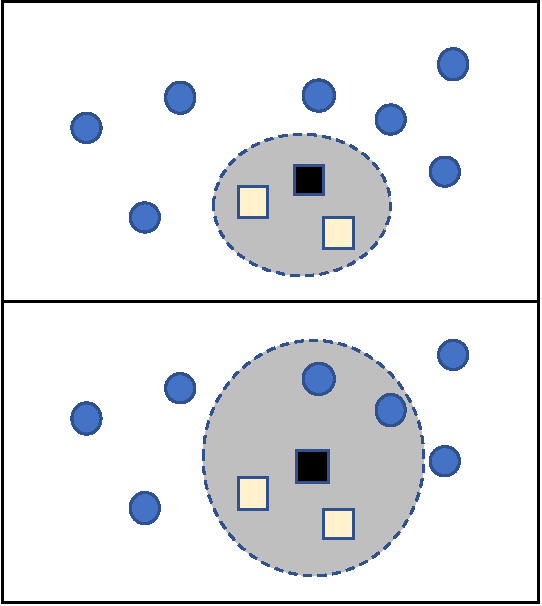
\includegraphics[width=1.5in]{imgs/bln/neighborhood.pdf}
    \caption{Unbalanced (top) and balanced (bottom) neighborhoods}
    \label{fig:neighbor}
\end{figure}

To enhance the degree of C-fairness in such a context, we introduce the notion of a \textit{balanced neighborhood}. A balanced neighborhood is one in which recommendations for all users are generated from neighborhoods that are balanced with respect to the protected and unprotected classes. This is shown in the bottom half of Figure~\ref{fig:neighbor}. The target has an equal number of peers inside and outside of the protected class. In the case of job recommendation discussed above, this would mean that female job seekers get recommendations from some female and some male peers.

There are a variety of ways that balanced neighborhoods might be formed. The simplest way would be to create neighborhoods for each user that balance accuracy against group membership. However, this would be highly computationally inefficient, requiring the solution of a separate optimization problem for each user. 

In this research, we explore an extension of the well-known Sparse Linear Method (SLIM)~\cite{ning2011slim}. SLIM is well-known as a state-of-the-art technology for collaborative recommendation. It is a generalization of item-based recommendation in which a regression coefficient is learned for each $\langle user, item \rangle$ pair. It can be slower to optimize than factorization-based methods, but for our purposes, it has the important benefit that the learned coefficients are readily interpretable with regard to group membership. Our extension of SLIM uses regularization to control the way different neighbors are weighted, with the goal of achieving balance between protected and non-protected neighbors for each user.

\subsubsection{\textbf{Sparse Linear Method}}
\hfill

SLIM learns $\langle user, item \rangle$ regression weights through optimization, minimizing a regularized loss function. Although this is not proposed in the original SLIM paper, it is possible to create a user-based version of SLIM (labeled SLIM-U in~\cite{zheng2014cslim}), which generalizes the user-based algorithm in the same way. 

Assume that there are $M$ users (a set $U$), $N$ items (a set $I$), and let us denote the associated 2-dimensional rating matrix by $R$. SLIM is designed for item ranking and therefore $R$ is typically binary. We will relax that requirement in this work, We use $u_i$ to denote user $i$ and $t_j$ to denote the item $j$. An entry, $r_{ij}$, in matrix $R$ represents the rating of $u_i$ on $t_j$.

SLIM-U predicts the ranking score $\hat{s}$ for a given user, item pair $\langle u_i, t_j \rangle$ as a weighted sum:

\begin{equation}
    \hat{s}_{ij} = \sum_{k \in U}{w_{ik}r_{kj}}, 
\end{equation}
where $w_{ii} = 0$ and $w_{ik} >= 0$.

Alternatively, this can be expressed as a matrix operation yielding the entire prediction matrix $\hat{S}$:    
\begin{equation}
\hat{S} = WR,
\end{equation}
where $W$ is an $M x M$ matrix of user-user weights. For efficiency, it is very important that this matrix be sparse.

The optimal weights for SLIM-U can be derived by solving the following minimization problem:

\begin{equation}
\mbox{min}_W \frac{1}{2}\left\Vert R - WR \right\Vert^2 + 
    \lambda_1 \left\Vert W \right\Vert^1 +
    \frac{\lambda_2}{2}\left\Vert W \right\Vert^2,   
\end{equation}
subject to $W > 0$  and $diag(W) = 0$.

The $\left\Vert W \right\Vert^2$ term represents the $\ell_2$ norm of the $W$ matrix and $\left\Vert W \right\Vert^1$ represents the $\ell_1$ norm. These regularization terms are present to constrain the optimization to prefer sparse sets of weights. Typically, coordinate descent is used for optimization. Refer to \cite{ning2011slim} for additional details. 

% \subsubsection{Neighborhood Balance}
\paragraph{\textbf{Neighborhood Balance}}

Recall that our aim in fair recommendation is to eliminate segregated recommendation neighborhoods where protected class users only receive recommendations from other users in the same class. Such neighborhoods would tend to magnify any biases present in the system. If users in the protected class only are recommended certain items, then they will be more likely to click on those items and thus increase the likelihood that the collaborative system will make these items the ones that others in the protected group see.

To reduce the probability that such neighborhoods will form, we use the SLIM-U formalization of the recommendation problem, but we add another regularization term to the loss function, which we call the \textit{neighborhood balance} term. To describe this term, we will enrich our notation further by indicating $U^+$ to be the subset of $U$ containing users in the protected class with the remaining users in the class $U^-$. Let $W_i^+$ be the set of weights for users in $U^+$ and $W_i^-$ be the corresponding set of weights for the non-protected class. Then the neighborhood balance term $b_i$ for a given user $i$ is the squared difference between the weights assigned to peers in the protected class versus the unprotected class.

\begin{equation}
    b_i = (\sum_{w^+ \in W_i^+}{w^+} - \sum_{w^- \in W_i^-}{w^-})^2
\end{equation}

A low value for the neighborhood balance term means that the user's predictions will be generated by weighting protected and unprotected users on a relatively equal basis.\footnote{Note that this is a class-blind optimization that tries to build balanced neighborhoods for both the protected and unprotected users. It is also possible to formulate the objective such that it only impacts the protected class and we leave this option for future work.}

Another way to express this idea is to create a vector $p$ of dimension $M$. If $u_i$ is in $U^+$, then $p_i = 1$; if $u_i$ is in $U^-$, then $p_i = -1$. Then, the sum expressed above can be rewritten as $b_i = (p^T \cdot w_i)^2$. By adding up this term for all users and adding it to the loss function, we can allow the optimization process to derive weights with neighborhood balance in mind. This adapted version of SLIM-U we will call \textit{Balanced Neighborhood SLIM-U} or BN-SLIM-U.

As in the case of the original SLIM implementation, we can apply the method of coordinate descent to optimize the objective. The full loss function is as follows:

\begin{equation}
\begin{split}
 L = \frac{1}{2}\left\Vert R - WR \right\Vert^2 + 
    \lambda_1 \left\Vert W \right\Vert^1 + 
    \frac{\lambda_2}{2}\left\Vert W \right\Vert^2 + \\
    \frac{\lambda_3}{2}\sum_{i \in U}\left(\sum_{k \in U}p_iw_{ik}\right)^2,
\end{split}
\end{equation}
where $w_{ii}=0$ and $w_{ik}>=0$ and where $\lambda_3$ is a parameter controlling the influence of the neighborhood balance calculation on the overall optimization

This loss function retains the property of the original SLIM algorithm in that the rows of the weight matrix are independent, and the weights in each row (those for each user) can be optimized independently. The algorithm chooses one $w_{ik}$ weight and solves the optimization problem for that weight, repeating over all the weights until convergence is reached. If we take the derivative of $L$ with respect to a single weight $w_{ik}$, we obtain

\begin{equation}\label{eq:derivative}
\begin{split}
\frac{\partial L_i}{\partial w_{ik}} = \sum_{j \in I}{(r_{ij} - 
    \sum_{l \in U'}{w_{il}r_{lj}})} + w_{ik}\sum_{j \in I}{r_{kj}^2} +  \\
    \lambda_1 + \lambda_2w_{ik} + \lambda_3p_k\sum_{l \in U'}{p_lw_{il}} 
\end{split}
\end{equation}
where $U' = U - \{u_i, u_k\}$.

We then set this derivative to zero and solve for the value of $w_{ik}$ that produces this minimum. This becomes the coordinate descent update step. 

\begin{equation}\label{eq:update}
\begin{split}
    w_{ik} \leftarrow \frac{S\left(X_{ik}, \lambda_1\right)_+}
    {\sum_{j \in I}{r_{kj}^2} + \lambda_2 + \lambda_3} \\
    X_{ik} = \sum_{j \in I}{(r_{ij} - 
    \sum_{l \in U'}{w_{il}r_{lj}})}+\lambda_3p_k\sum_{l \in U'}{p_lw_{il}}
\end{split}
\end{equation}
where $S()_+$ is the soft threshold operator defined in ~\cite{friedman_pathwise_2007}.

\paragraph{\textbf{Item-based neighborhoods}}

As noted above, some applications may require P-fairness: making the recommendation outcomes fair relative to the items being recommended. In our micro-finance example, the operators of this site have the goal of providing equal exposure to loans from different geographic regions. To address the P-fairness case, we can use an analogous approach using item neighborhoods and item weights, ensuring that items in a protected group are in neighborhoods that have balanced membership of items from the unprotected group. The derivation of the loss function is exactly analogous, yielding another variant of the SLIM algorithm that we refer to as \textit{Balanced Neighborhood SLIM} or BN-SLIM.

\subsubsection{\textbf{Methodology}}
\hfill

In order to evaluate our balanced neighborhood approach, we conducted separate sets of experiments in both consumer- and provider-fairness. It is very difficult to find datasets that contain the kind of features that would be necessary to evaluate fairness-aware recommendation algorithms, especially related to user demographics in sensitive application areas such as employment. 

For the purposes of this paper, we are using the well-known MovieLens 1M dataset~\cite{movielens}, which contains gender information for each user, as well as ratings of 4,000 movies by 6,000 users. Movie recommendation is, of course, a domain of pure individual taste and therefore not an obvious candidate for fairness-aware recommendation. Following the example of \cite{yao2017beyond}, our approach to construct an artificial equity scenario within this data for expository purposes only, with the understanding that real scenarios can be approached with a similar methodology. 

Our consumer-fairness scenario centers on movie genres. It can be seen in this data that there is a minority of female users (1709 out of the total of 6040). Certain genres display a discrepancy in recommendation delivery to male and female users. For example, in the ``Crime'' genre, female users rate a very similar number of movies (average of 0.048\% of female profiles vs 0.049\% of male profiles) and rate them similarly: an average rating of 3.7 for both female and male users. However, our baseline unmodified SLIM-U algorithm recommends in the top 10 an average of 1.10 ``Crime'' movies per female user as opposed to 1.18 such movies to male users. We are still exploring the cause of this discrepancy, but it seems likely that there are influential female users with a lower opinion of this genre. 

Given that the rating profiles are similar but the recommendation outcomes are different, we can therefore conclude that the female users experience a deprivation of ``Crime'' movies compared to their male counter-parts. Similar losses can be observed for other genres. We are not asserting that there is any harm associated with this outcome. It is sufficient that these differences allow us to validate the properties of the BN-SLIM-U algorithm.

Our goal, then, is to reduce or eliminate genre discrepancies with minimal accuracy loss by constructing balanced neighborhoods for the MovieLens users. The $p$ vector in Equation~\ref{eq:update} therefore will have a 1 for female users and a -1 for male users. In the experiments below, we compare the user-based SLIM algorithm in its unmodified form and the balanced neighborhood version BN-SLIM-U.

In evaluating fairness of outcome, we use a variant of what is known in statistics as \textit{risk ratio} or \textit{relative risk} (RR)\cite{romei2014multidisciplinary}. We measure what is effectively \textit{relative opportunity}. In other words, we measure the observed probability of protected class items being recommended divided by the probability of unprotected class items being recommended. In our MovieLens experiments, we measure the number of movies in protected and unprotected genres included in recommendation lists  as the measure of outcome quality. We construct a consumer-side equity score, $E_c@k$ for recommendation lists of k items, as the ratio between the outcomes for the different groups. Let $P_i@k = {\rho_1, \rho_2, ..., \rho_k}$ be the top $k$ recommendation list for user $i$, and let $\gamma()$ be a function $\rho \rightarrow \{0,1\}$ that maps to 1 if the recommended movie is in a protected genre. Then:

\begin{equation}
E_c@k=\frac{\sum_{i \in U^+}{\sum_{\rho \in P_i@k}{\gamma(\rho)}}/|U^+|}
{\sum_{i \in U^-}{\sum_{\rho \in P_i@k}{\gamma(\rho)}}/|U^-|}
\end{equation}

$E_c@k$ will be less than 1 when the protected group is, on average, recommended fewer movies of the desired genre. It may be unrealistic to imagine that this value should approach 1: the metric does not correct for other factors that might influence this score -- for example, female users may rate a particular genre significantly lower and an equality of outcome should not be expected. While the absolute value of the metric may be difficult to interpret, it is still useful for comparing algorithms. The one with the higher $E_c@k$ is providing more movies in the given genre to the protected group. Note that this is an additive, utilitarian measure of outcome equity and does not take into account variations in user experience. More nuanced measures of distributional equity, including Pareto improvement, we leave for future work.

As in any multi-criteria setting, we must be concerned about any loss of accuracy that results from taking additional criteria into consideration. Therefore, we also evaluate the ranking accuracy of our algorithms in the results below. The measure that we use is normalized discounted cumulative gain (NDCG) measured at a specific list length. In this measure, an item appearing on a recommendation list accrues ``gain'' according to its position on the list -- thus the discount. The measure is normalized by comparing the algorithm's performance to the best ranking that could have been achieved. 

Let $P_i@10$ be a list of retrieved list of length 10 and let $\tau$ be an indicator function that is 1 for movies that the user liked and 0 for others. Then, DCG@10 is computed as

\begin{equation}
DCG@10 = \sum_{k=1}^{10}{\frac{\tau(\rho_k)}{log_2(k+1)}}
\end{equation}

NDCG@10 is this DCG@10 value divided by the optimal DCG, which occurs when all of the movies liked by the user and appearing the test set are ranked at the top of the list in their order of preference.

\paragraph{\textbf{Provider fairness}}

To evaluate our approach for provider fairness, we are using a dataset extracted from the Kiva.org microlending site using the site's API\footnote{http://build.kiva.org/}. Again, we have constructed our own scenario using this data, focusing on geographic region. In our dataset, we find that there are some geographic regions with a higher than average number of unfunded loans. In these regions, borrowers have a lower probability of getting the desired capital. See Table~\ref{tab:unfunded}.

\begin{table}
    \centering
\begin{tabular}{l|l|r}
    Category & Region & Unfunded \% \\ \hline
    Unprotected & North America & 1.73 \\
    & Eastern Europe & 0.99 \\
    & South America & 4.33 \\
    & Asia & 6.70 \\ \hline
    Protected & Africa & 10.57 \\
    & Middle East & 13.23 \\
    & Central America & 8.81 \\
\end{tabular}
    \caption{Percentage of unfunded loans by region}
    \label{tab:unfunded}
\end{table}

For the purposes of our experiments, we will assume that one of the goals of a microlending site is to equalize access to capital across geographic regions. Kiva does not currently offer personalized recommendation of loans to its users, but if it did, a fairness-aware recommendation approach could be used to promote the loans of borrowers in the underserved regions. 

We will therefore treat the under-represented regions collectively as the protected group and the other regions as the unprotected group. This enables us to use our item-based neighborhood balance algorithm described above. A more fine-grained approach to geographic equity that tries to balance across all regions would require additional algorithmic development and is left for future work. 

Again, we will represent fairness as a ratio of outcomes. It is simpler to compute in this case, as we are not dividing the recommendations by genre. The provider-side equity score, $E_p@k$, is defined on recommendation lists of k items. Let $L^+$ be the set of loans in the test set that are from the protected regions, and $L^-$ be the corresponding set from the unprotected regions. Also, let $\pi^+()$ be an indicator function $\rho \rightarrow \{0,1\}$ that maps to 1 if the recommended loan is from a protected region and $\pi^-$ is a similar function for the unprotected regions. Then:

\begin{equation}
E_p@k=\frac{\sum_{i \in U}{\sum_{\rho \in P_i@k}{\pi^+(\rho)}}/|L^+|}
{\sum_{i \in U}{\sum_{\rho \in P_i@k}{\pi^-(\rho)}}/|L^-|}
\end{equation}

$E_p@k$ will be less than 1 when loans from the protected regions are appearing less often on recommendation lists. As with $E_c$, this is a utilitarian measure, summing over all borrower regions, and does not speak to the the distribution across individual borrowers. Like $E_c$, it does not take the rank of recommended items into account.

\subsubsection{\textbf{Results}}
\hfill

We implemented the SLIM-U, BN-SLIM, and BN-SLIM-U algorithms using LibRec 2.0~\cite{guo2015librec}, and used its existing implementation of SLIM. We used 5-fold cross-validation as implemented within the library.

\paragraph{\textbf{Consumer fairness: MovieLens}}

Within the MovieLens 1M dataset, we selected the five genres on which the SLIM-U algorithm produced the lowest equity scores: ``Film-Noir'', ``Mystery'', ``Horror'', ``Documentary'', and ``Crime''. The parameters were set as follows: $\lambda_1 = 0.1$, $\lambda_2 = 0.001$, and (for BN-SLIM-U) $\lambda_3 = 25$\footnote{Because the balance term measures the difference in weights, it tends to be much smaller than the terms that measure the sums of weights. Therefore, the regularization constant must be much higher for the balance term to have an impact on the optimization.}. 

\begin{figure}[tbh]
    \centering
    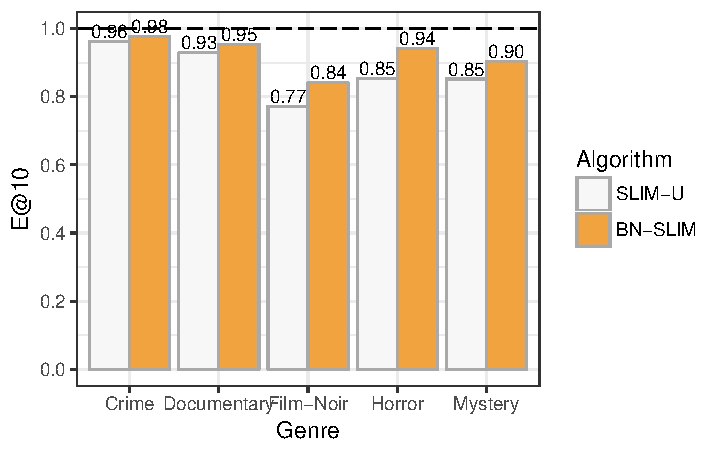
\includegraphics[width=3.00in]{imgs/bln/genre-compare3.pdf}
    \caption{Equity score for SLIM-U and BN-SLIM-U. Line indicates equal percentage across genders}
    \label{fig:genre}
\end{figure}

Figure~\ref{fig:genre} shows the results of the experiment in terms of the equity scores for each genre. Perfect equity (1.0) is marked with the dashed line. As we can see, in every case, the balanced neighborhood algorithm produced an equity score closer to 1.0 than the unmodified algorithm. The largest jump is seen in the ``Horror'' genre, about 0.09 in the equity score or around 10\%.

In terms of accuracy, there was only a small loss of NDCG@10 between the two conditions. See Table~\ref{tab:ndcg}. The difference amounts to approximately 2\% loss in NDCG@10 for the balanced neighborhood version.

\begin{table}
\centering
\begin{tabular}{c|c}
    Algorithm &  NDCG@10 \\ \hline
    SLIM-U & 0.053 \\ \hline
    BN-SLIM & 0.052 \\ \hline
\end{tabular}
\caption{Ranking accuracy}
\label{tab:ndcg}
\end{table}

Because the balanced neighborhood algorithm is applied across all users, it also has the effect of showing male users movie genres that occur more frequently for female users. To see this effect, we examined the five genres with the highest $E_c@10$ values: ``Fantasy'', ``Animation'', ``War'', ``Romance'', and ``Western'' using the same parameter values as above. The results appear in Figure~\ref{fig:inverse-equity} and show a similar result. ``War'' is something of an anomaly here, both because it is perhaps unexpected to see it as a one of the more female-recommended genres and because the genre-balance algorithm pushes it to become more skewed rather than less. We are investigating the cause of this phenomenon. Overall, the BN-SLIM-U algorithm produces a recommendation experience in which the occurrence of gender-specific genres is more closely equalized, with small loss in ranking accuracy. 

\begin{figure}[bth]
    \centering
    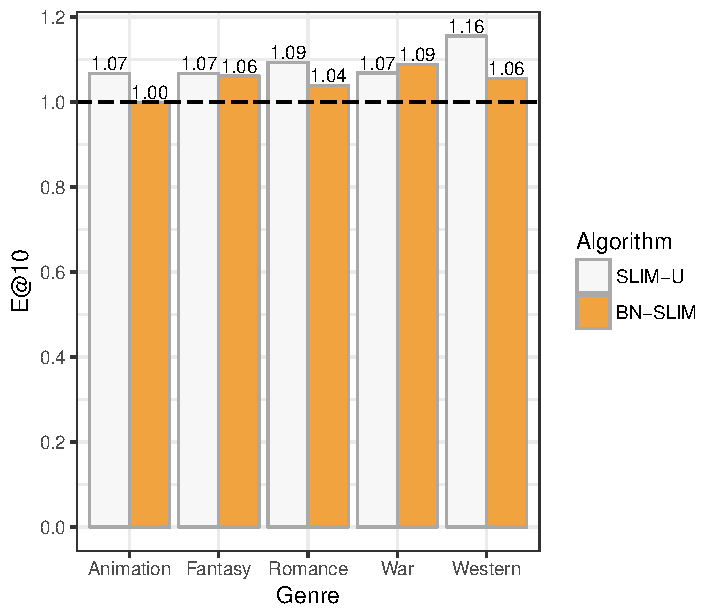
\includegraphics[width=3in]{imgs/bln/inverse-genres3.pdf}
    \caption{Equity scores for female-preferred genres}
    \label{fig:inverse-equity}
\end{figure}

\paragraph{\textbf{Provider fairness: Kiva.org}}
Our dataset was extracted from Kiva's public API in September of 2016 and contains approximately 1 million loans funded by approximately 180,000 lenders. One challenge for collaborative recommendation in the microlending area is that loans are generally one-time endeavors. Unlike a movie that can be watched by an unrestricted number of viewers, a loan -- once funded -- disappears from Kiva.org and is not available for other lenders to view or support. Most loans are supported by from 1-330 lenders, by contrast, a popular movie in the MovieLens dataset might be rated by thousands of users. Thus, the lender-borrower relation is highly sparse, and loans have very small profiles.

To be able to apply the SLIM algorithm, we used a hybrid recommendation technique incorporating content data in the form of loan characteristics. We characterized each loan using five characteristics available from Kiva: borrower gender, borrower country, loan sector, loan purpose, and loan amount. Each of the original 1 million loan identifiers in the database was replaced with a psuedo-item identifier corresponding to the appropriate combination of loan characteristics. A 5-core transformation was then applied to the dataset, retaining only those users who had funded at least 5 psuedo-items and those psuedo-items with at least 5 funders. The retained dataset has 3,593 psuedo-items, 29,342 users and 393,035 ratings.

Kiva.org divides its borrowers into 9 geographic regions. As discussed above, for the purposes of this paper we are defining the protected group as those regions of the world where it appears to be more difficult to fund loans. (In Kiva.org, a loan that does not attract enough lenders over a 30 day period is marked as unfunded and dropped from the system.) As shown in Table~\ref{tab:unfunded}, the regions of North America, Eastern Europe, South America, and Asia have proportionately more funded loans than the regions of Africa, Middle East, and Central America\footnote{Our data set had only a single loan request from Australia.}. These regions where borrowers have lower funding percentages are treated as the protected group in our experiments.

With this transformation in place, it was possible to apply the SLIM algorithm and generate personalized recommendations. The regularization parameters were set as follows: $\lambda_1 = 0.01$ and $\lambda_2 = 0.001$. For BN-SLIM, $\lambda_3$ had a value of 0.9. Table~\ref{tab:results} shows the performance of the these algorithms in the provider fairness condition. Interestingly, the ranking accuracy, as measured by NDCG@10, actually increases between the conditions, indicating that the balanced neighborhood condition actually yields better recommendation lists than the unmodified SLIM algorithm. In addition, the $E_p@10$ value, which is unbalanced at 0.90 for SLIM is improved to close to 1.0, the equity target that we were aiming for.

\begin{table}
    \centering
\begin{tabular}{l|r|r}
    Algorithm & NDCG@10 & $E_p@10$ \\ \hline
    SLIM & 0.046 & 0.90 \\ \hline
    BN-SLIM & 0.049 & 1.05 \\ \hline
\end{tabular}
    \caption{Comparison of algorithm performance}
    \label{tab:results}
\end{table}


% \subsubsection{\textbf{Close Related Work}}
% There has been relatively little work on fairness in recommender systems.
% Most researchers in the area have defined fairness in terms of differing levels of accuracy for different classes of users. See, for example, \cite{DBLP:conf/recsys/KamishimaAAS14,kamisha-akaho-fatrec-2017,yao_huang_fatml-2017}. 

% As noted above, some special cases of provider-side fairness have been studied in the context of diversity-aware and long-tail recommendation. See, for example, \cite{Zhang:2008:AMI:1454008.1454030,adomavicius2012improving,o2004preserving,adomavicius2012improving}. 
% Our BN-SLIM algorithm can be seen as an approach to building systems that target particular diversity-aware recommendation problems, where the providers and/or items can be divided into two disjoint categories. However, the approach is particularly suited to fairness-aware contexts because the objective function is optimized precisely when the protected and unprotected groups are weighted the same by the algorithm. 

% The most obvious precursor for this research is the work of Dwork et al. in the area of fair representation~\cite{zemel2013learning,fairness}. The authors propose learning a mapping between the individual instances in the data to prototype instances with balanced membership such that protected group identities are not recoverable. Our application of this concept is different in that we are building on the standard nearest neighbor techniques in recommender systems and building balanced neighborhoods to ensure diversity among the peers from whom recommendations are generated. 

\subsubsection{\textbf{Conclusion and Future Work}}

% This paper extends ideas of fairness in classification to personalized recommendation. 
Our BN-SLIM algorithm can be seen as an approach to building systems that target particular diversity-aware recommendation problems, where the providers and/or items can be divided into two disjoint categories. However, the approach is particularly suited to fairness-aware contexts because the objective function is optimized precisely when the protected and unprotected groups are weighted the same by the algorithm. 

The most obvious precursor for this research is the work of Dwork et al. in the area of fair representation~\cite{zemel2013learning,fairness}. The authors propose learning a mapping between the individual instances in the data to prototype instances with balanced membership such that protected group identities are not recoverable. 

This paper extends this idea of fairness in classification to personalized recommendation. However, our application of this concept is different in that we are building on the standard nearest neighbor techniques in recommender systems and building balanced neighborhoods to ensure diversity among the peers from whom recommendations are generated. 

A key aspect of this extension is to note the tension between a personalized view of recommendation delivery and a regulatory view that values particular outcomes. The regulatory view is somewhat foreign to research in personalization, but there are strong arguments that total obedience to user preference is not always risk-free or desirable~\cite{pariser2011filter,sunstein2009republic}. This paper also introduces the concept of multisided fairness, relevant in multisided platforms that serve a matchmaking function. We identify consumer- and provider- fairness as properties desirable in certain applications and demonstrate that the concept of balanced neighborhoods in conjunction with the well-known sparse linear method can be used to balance personalization with fairness considerations.

In our future work, we plan to extend these findings in several ways. It is possible that a multisided platform may require fairness be considered for both consumers and providers at the same time: a CP-fairness condition. For example, a rental property recommender may treat minority applicants as a protected class and wish to ensure that they are recommended properties similar to unprotected renters. At the same time, the recommender may wish to treat minority landlords as a protected class and ensure that highly-qualified tenants are referred to them at the same rate as to landlords who are not in the protected class. One important question for future research is how the outcomes for each stakeholder and the overall system performance are affected by combining consumer- and provider-fairness concerns.
Another path to pursue is to have a more extensive experimentation of the fairness properties of the balanced neighborhood SLIM for both consumers and providers. We would like to test this idea on K-nearest neighbor method as well. Finally, we expect to publish a journal article of these thorough experiments in the Information and Management Journal.

% Another important area of research is to extend our measures of fairness. The additive measures used in this paper capture an aggregate representation of how recommendation results are changing for user and provider groups generally, but they do not permit fine-grained analysis of the tradeoffs experienced by individual users or providers. We do not know, for example, if the results of our Kiva.org experiments represent a Pareto improvement in system performance or just an average improvement over the stakeholder groups, and whether some subgroups are impacted more than others.

% One of the key challenges in this area is the domain-specificity of recommendation environments. The utilities that are delivered to each class of stakeholder are highly dependent on the type of item being recommended, the social function of the platform, and the interactions that it enables. It is therefore difficult to find appropriate data sets for experimentation and challenging to generalize across recommendation scenarios. 



\section{Re-ranking}
In this section, we focus on achieving provider fairness using a re-ranking approach.

The problem of promoting provider fairness while maintaining recommendation accuracy can be generally characterized as a multi-objective optimization problem. If optimal fairness and optimal recommendation accuracy could be achieved simultaneously, there would be no need for research in this area. However, optimizing recommendation accuracy often comes at the expense of provider fairness, due to various biases present in recommender systems, including popularity bias \cite{celma2008hits,lee2014fairness}, and user-base composition \cite{lin2019crank, yao2017beyond}. Research in provider fairness is therefore generally concerned with improving the tradeoff between fairness and accuracy, or in other words, increasing the amount of fairness that can be gained for a given degree of accuracy loss.

We motivate the problem in the context of loan recommendation where consumers are lenders and providers are borrowers. We propose two reranking methods: (1) Fairness-Aware Re-ranking (PFAR) and the personalized version of PFAR, and (2) Opportunistic Fairness-Aware Re-ranking (OFAiR).

%  try to increase the exposure of marginalized or protected borrowers. 
The re-ranking criterion can be regarded as modelling \textit{personalization} and \textit{fairness}, respectively, with a hyper-parameter $\lambda$ controlling the tradeoff between the two. We demonstrate that both methods achieve reasonable fairness / accuracy trade-offs and increase the exposure of the protected group(s) drastically. Although OFAiR achieves a better fairness / accuracy tradeoff compared to FAR/PFAR.


\subsection{Fair-Aware Re-ranking/Personalized Fair-Aware Re-ranking}

Microlending is the provision of small and low-interest loans (as little as \$25) to low-income individuals or small-scale entrepreneurs from under-developed countries  \cite{yunus1998banker}. The extremely poor people in rural areas often lack collateral, steady employment, or a verifiable credit history, hence they cannot get access to financial services. Under such circumstances, microlending has attracted an increased attention in the last decade \cite{chen2017microfinance}, providing impoverished entrepreneurs an opportunity to start their own businesses as well as avoid the vicious cycle of debt.

One of the leading international microlending organizations, Kiva Microfunds (Kiva.org), has crowd-funded about 3 million borrowers with \$1.27 billion USD as of February 2019 \cite{kiva}. Kiva does not collect interest but provides an intermediary service for lenders and borrowers, as illustrated in Figure \ref{fig:kiva_process}. Borrowers from over 80 countries, divided into 8 regions by Kiva, post their applications for loans on the website for lenders to support. Lenders browse and crowd-fund the loans in the increments of \$25 or more. 
%After 

% % recommender systems, personalization
Loan recommender systems \cite{choo2014gather,choo2014understanding} are designed to assist lenders in looking for promising borrowers. Such systems model lenders' historical behaviors and generate personalized recommendations to meet the lenders' interests or needs. While these recommender systems aim to provide efficient and personalized services, two issues are largely overlooked.

\begin{figure}
%\vspace{-0.25cm}
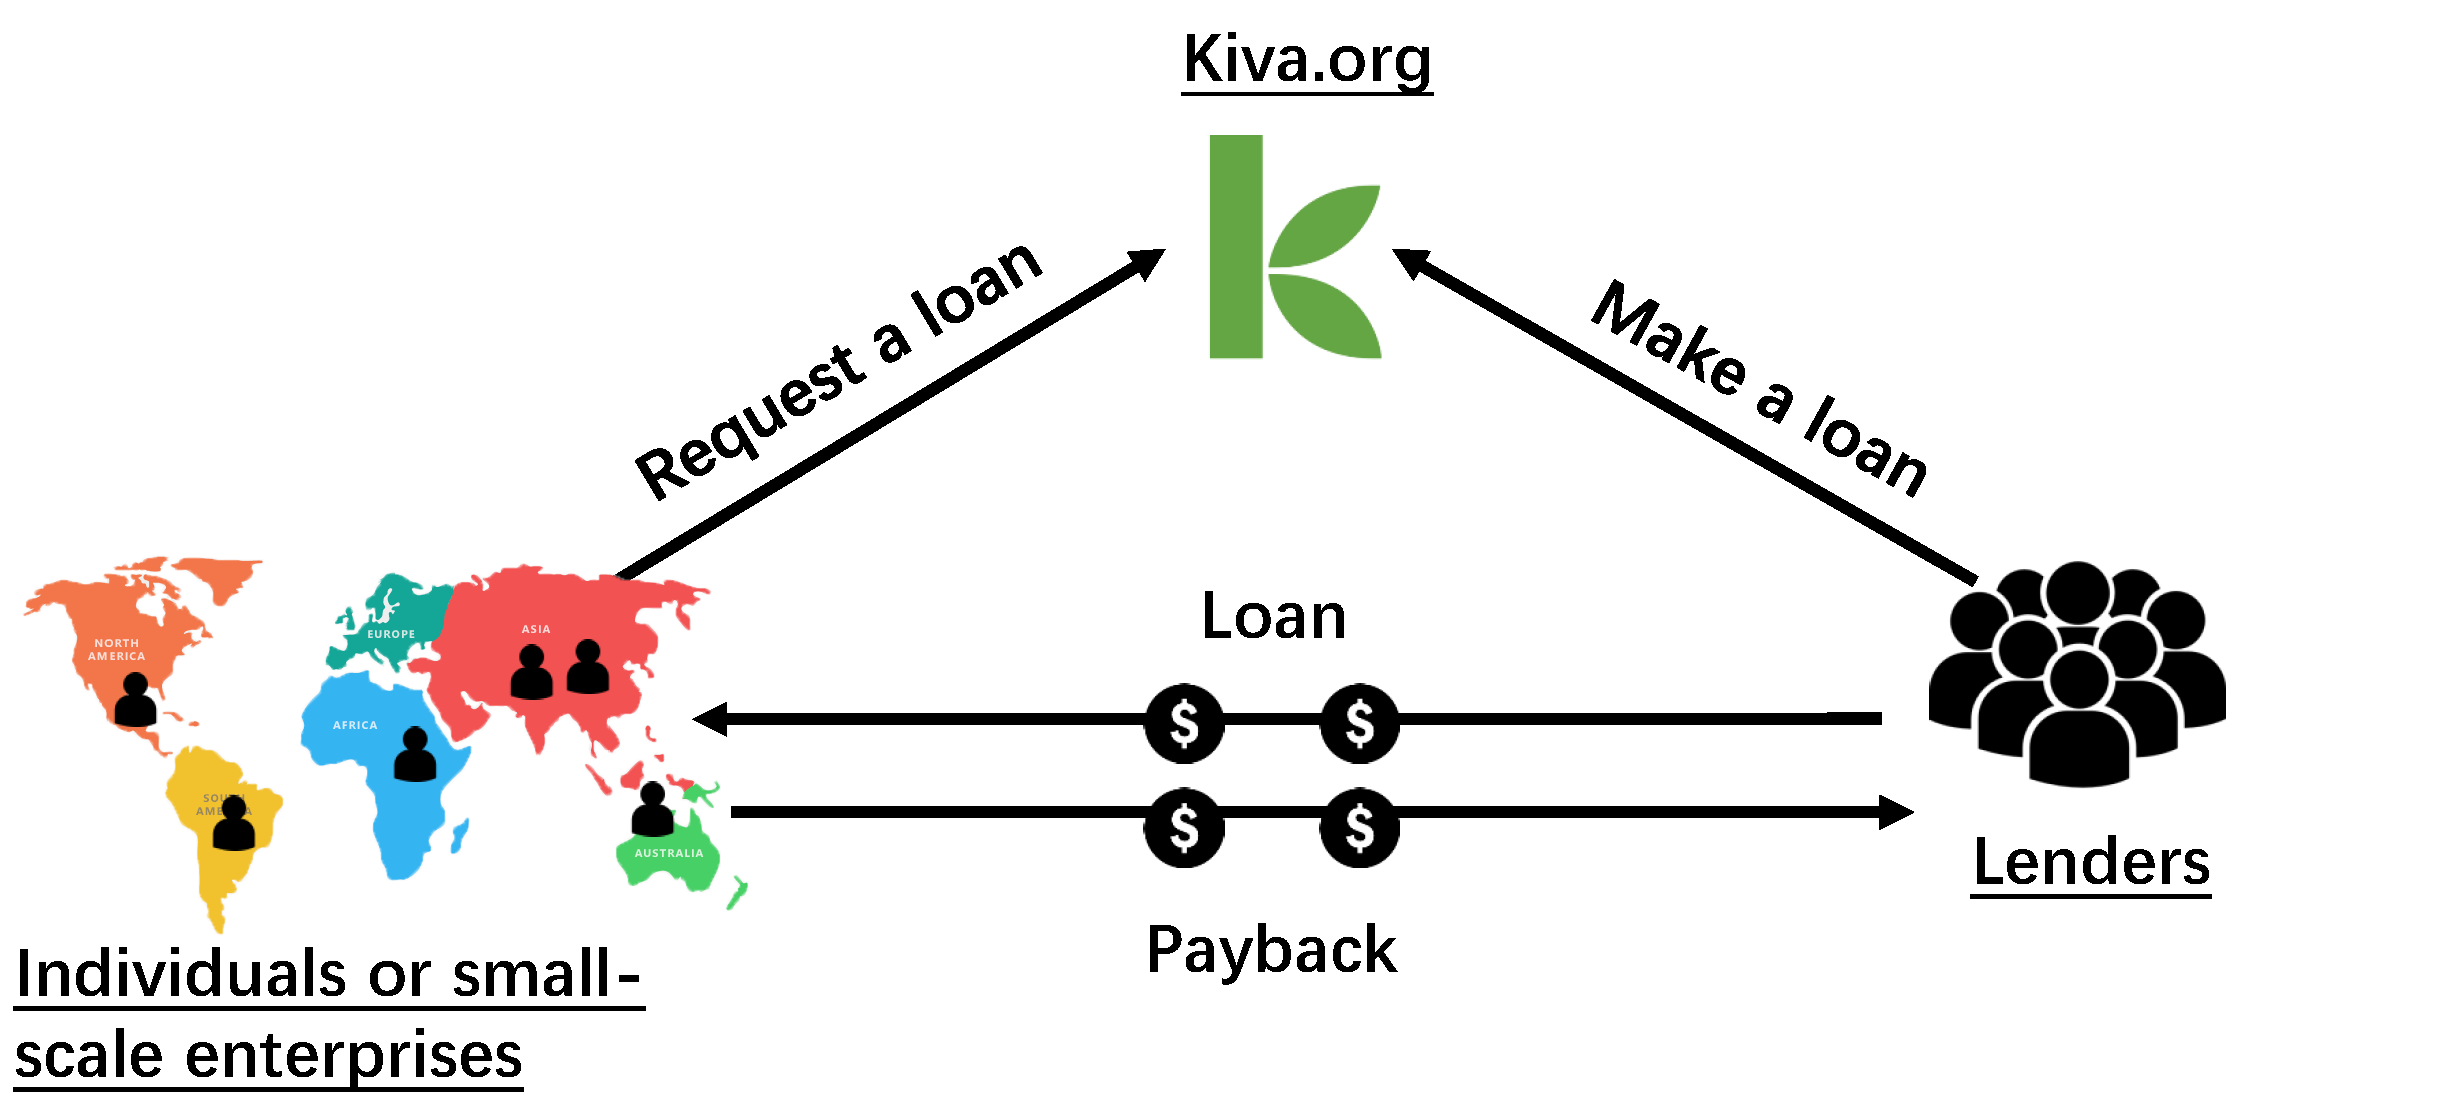
\includegraphics[width=0.98\columnwidth]{imgs/far/microlending.png}
%\vspace{-0.25cm}
\caption{Kiva.org provides an intermediary service for lenders and borrowers.}
\label{fig:kiva_process}
\end{figure}

\begin{figure}
%\vspace{-0.25cm}
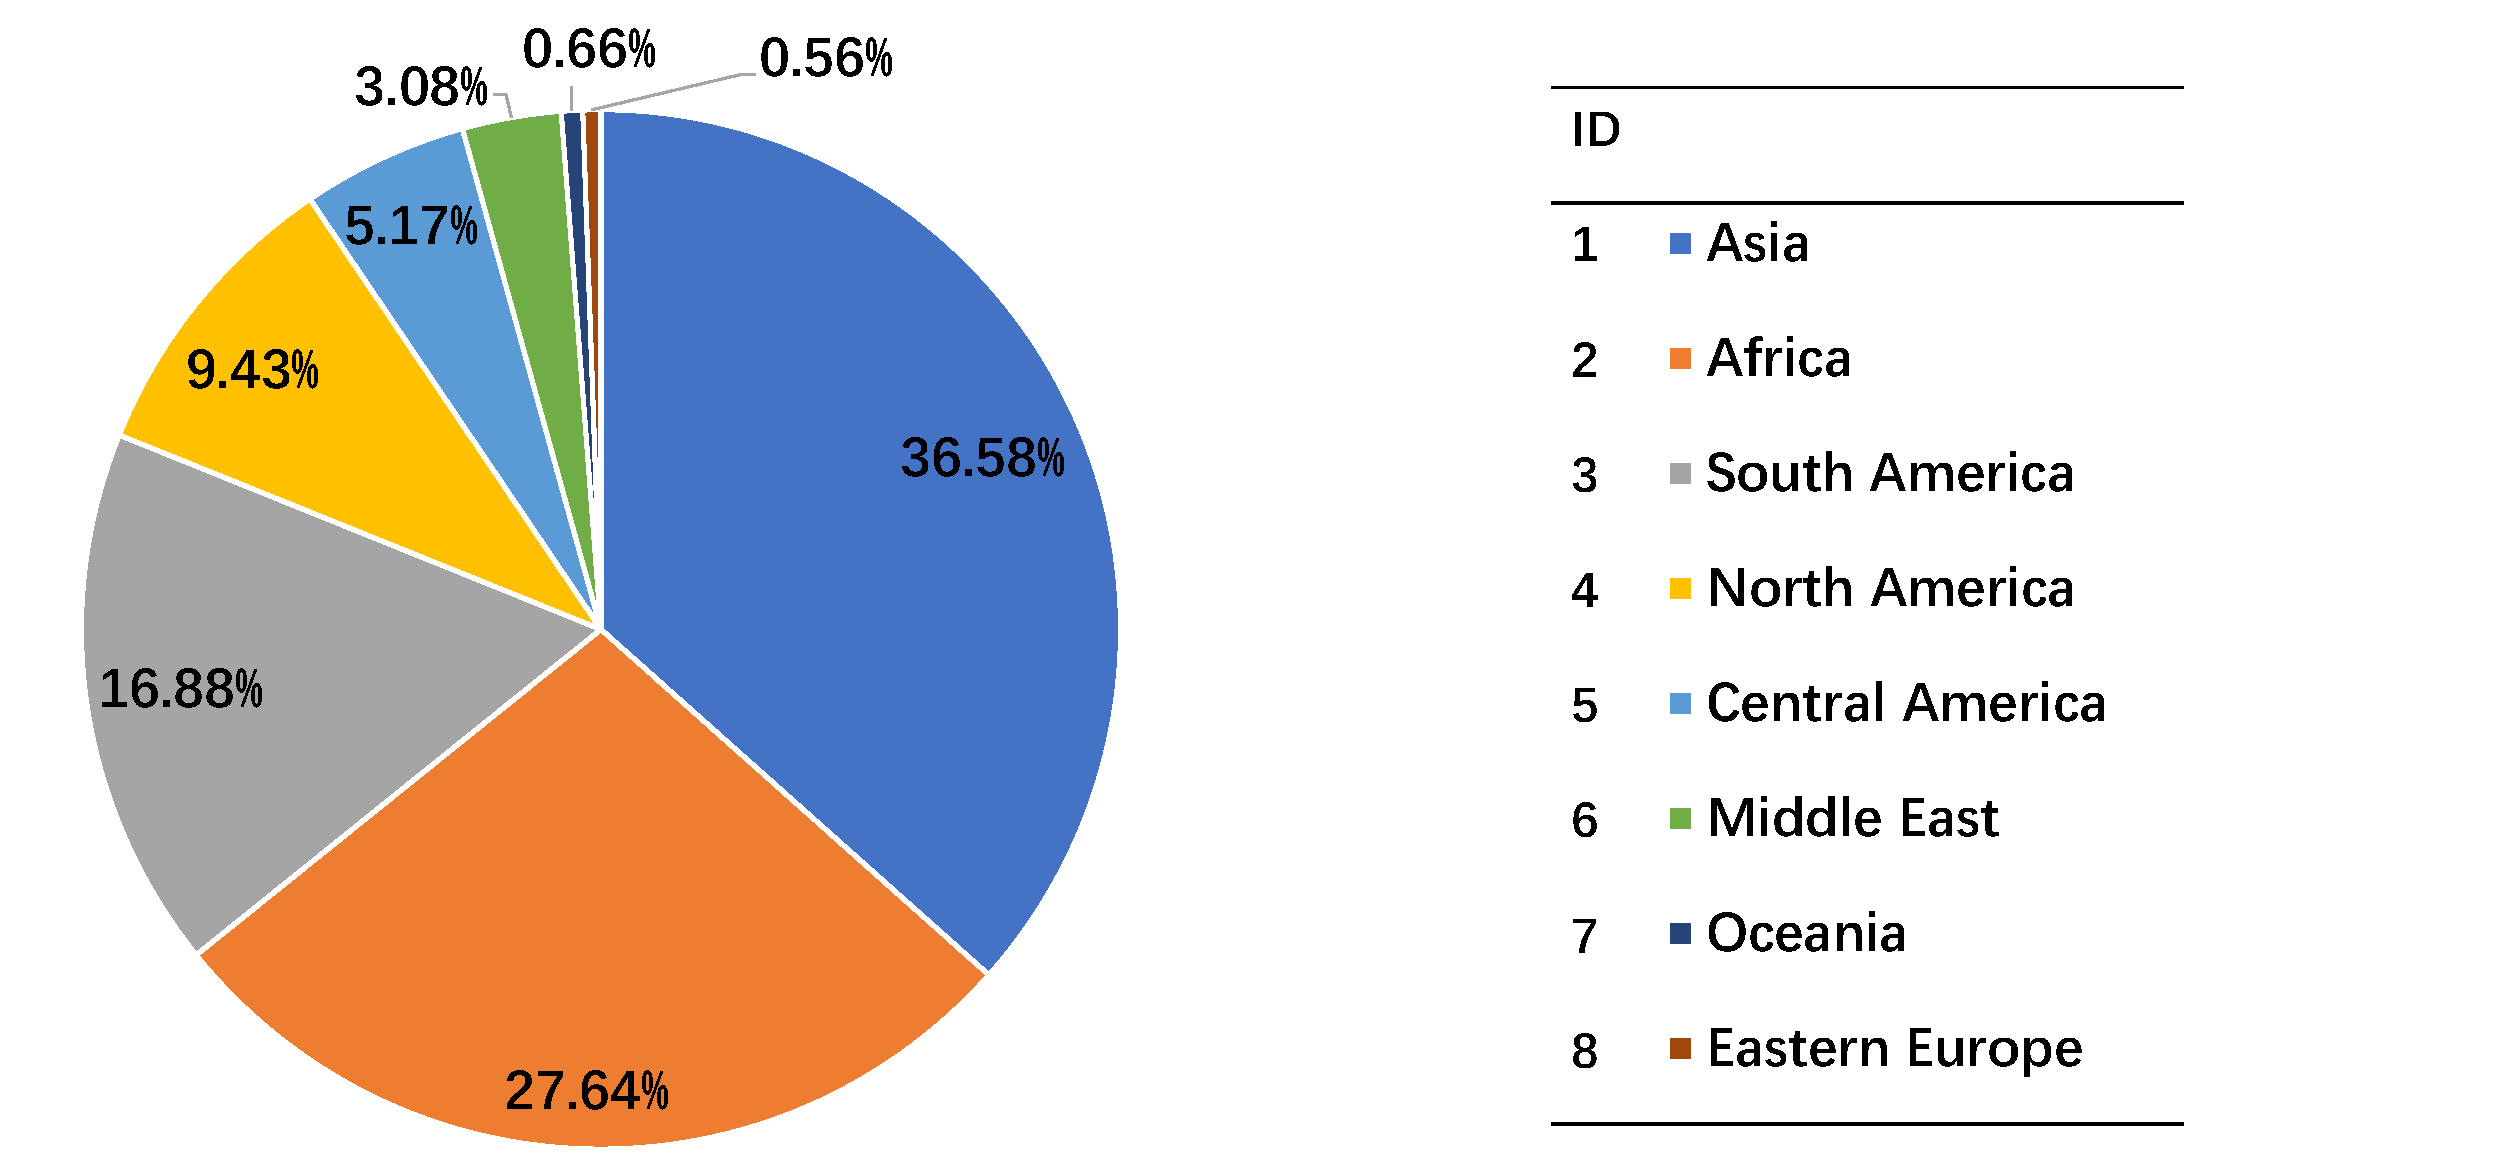
\includegraphics[width=0.98\columnwidth]{imgs/far/kiva.png}
%\vspace{-0.25cm}
\caption{The issue of fairness on regions in a designed loan recommender system \cite{choo2014gather} for Kiva: the recommendation percentage for each region.}
\label{fig:recom_result}
\end{figure}


(i) \textit{Unfair recommendation.} The existing recommender systems for microlending are all lender-centered. These recommender systems have been demonstrated to favor popular items \cite{celma2008hits,lee2014fairness}, resulting in extremely unbalanced recommendation results --- majority groups are usually over-represented, thereby holding a higher proportion of opportunities and resources, while minority groups barely receive exposure. For example, it is observed that certain geographical regions such as Asia and Africa dominate the recommendation in a designed loan recommender system for Kiva~\cite{choo2014gather}; whereas, others like Oceania and Eastern Europe barely receive recommendations, as shown in Figure \ref{fig:recom_result}. Less exposure means the borrowers from these regions are less likely to be funded.

%Moreover, the recommender system will learn the pattern from the historical data that loans from certain regions are less interested, thereby increasing the unfairness.

(ii) \textit{Lender's diversity tolerance.} Another noticeable phenomenon is that lenders' tolerance of diversity varies greatly.  Thus, the diversity of recommended lists should be compatible with the level of each lender's interest in diverse recommendations. For instance, some lenders may highly prefer offering loans to certain regions (such as their home countries), while others may be open to diverse regions. In such scenarios, assuming lenders' diversity tolerance is constant and increasing diversity uniformly for all lenders 
%to improve fairness 
will result in poor recommendations \cite{eskandanian2017clustering}. Therefore, a well-designed recommender system should be personalized by both lenders' interests and the degree of loan diversity in recommended lists.

We aim to design a fairness-aware re-ranking algorithm on top of the existing recommendation algorithms. Our algorithm achieves a balance between recommendation accuracy and borrower-side fairness, and also considers lenders' preferences for diversity. This post-processing step does not depend on any specific recommendation algorithm, and therefore can be widely applied.

% \todo{?}
% \citet{surer2018multistakeholder} suggest a constrained optimization-based method at the post-processing level to enhance fairness for multiple provider groups. This approach is generalizable to multiple constraints, such as a) the inclusion of items from different provider groups, b) ensuring a minimum degree of item diversity for each consumer, and, c) avoiding unfairness towards providers from underrepresented populations.

% \section{The Proposed Algorithm}\label{sect:algorithm}
In this section, we first propose to formulate this recommendation scenario as a Multi-sided Recommender System (MRS) \cite{burke2017multisided, burke2017patterns}.  Then, we design a personalized re-ranking algorithm to achieve a fair recommendation for microlending.

% \begin{figure}
% %\vspace{-0.25cm}
% 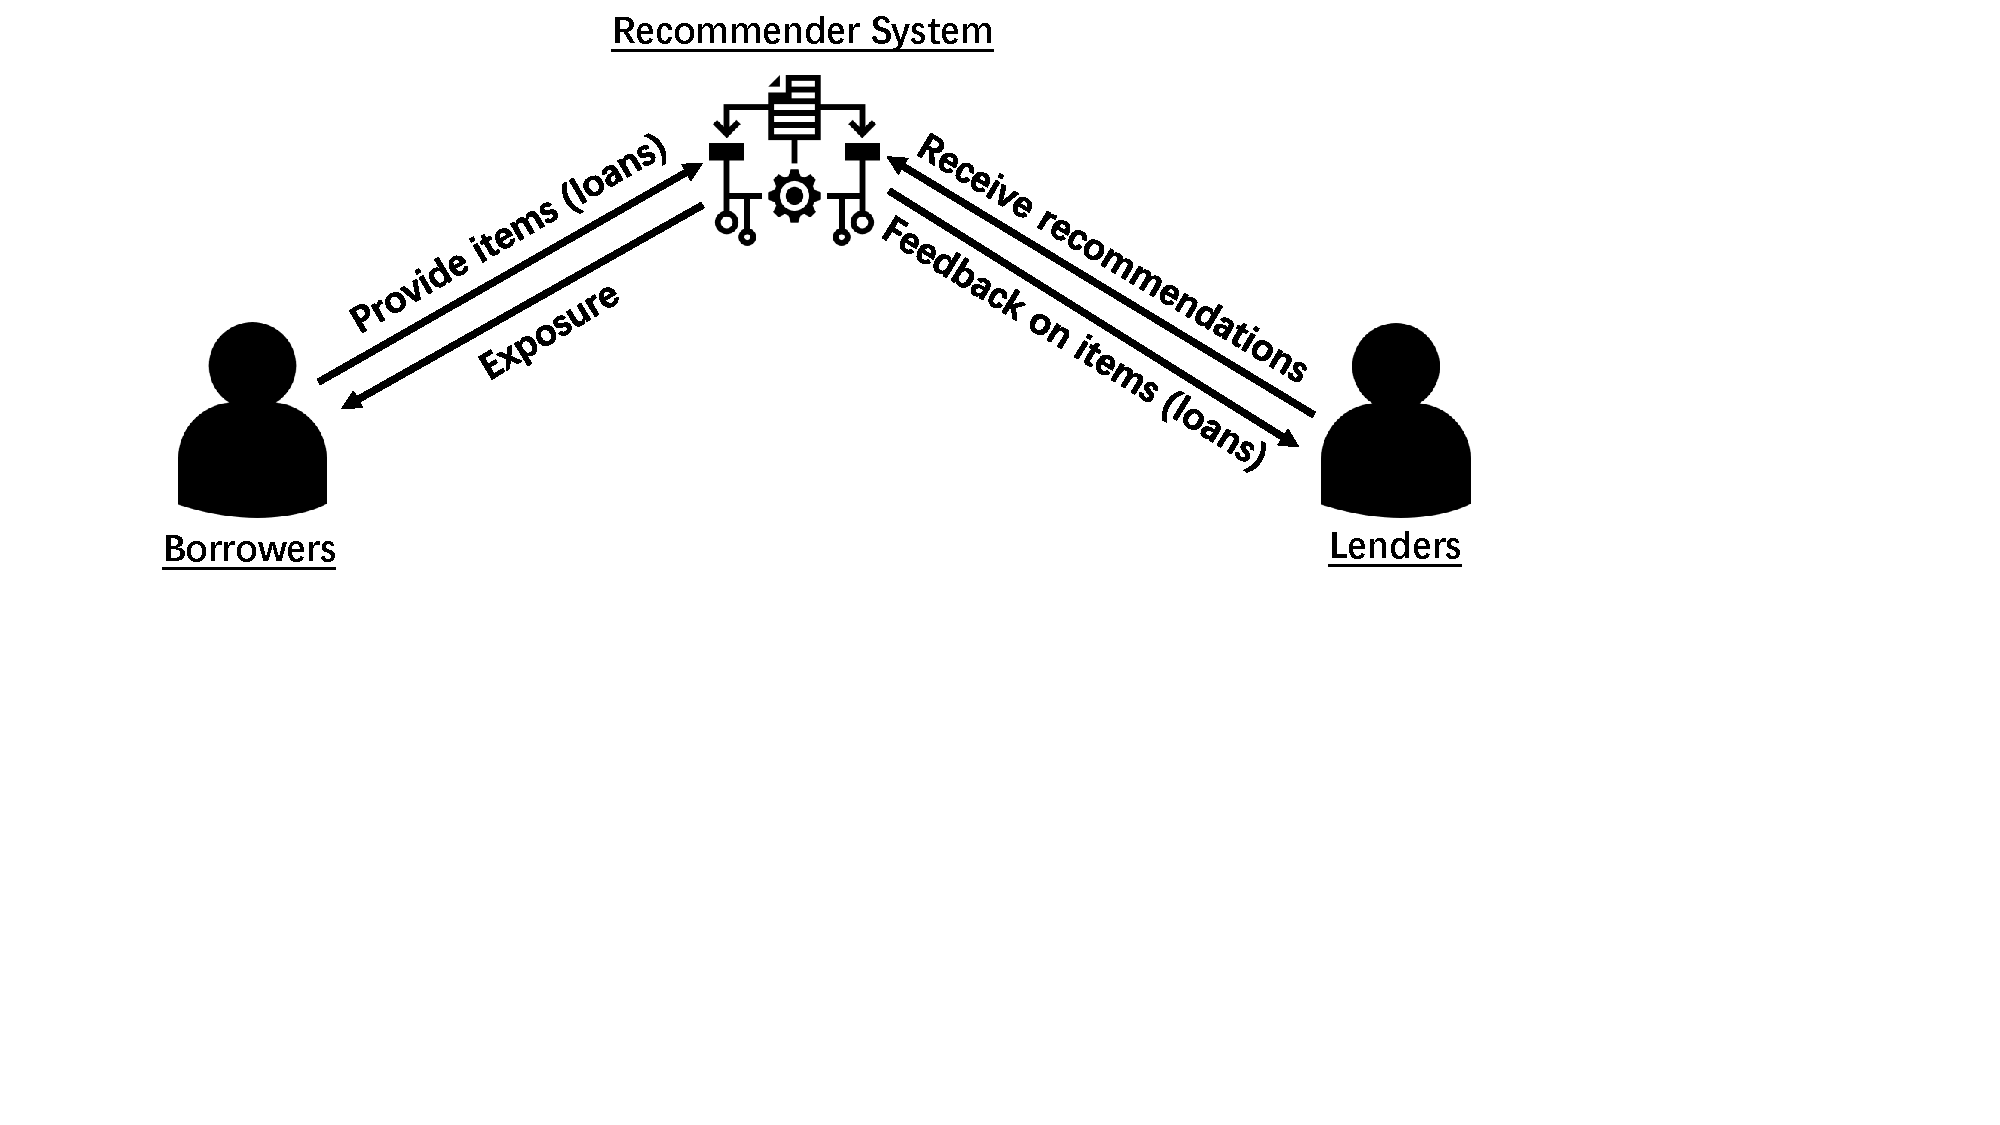
\includegraphics[width=0.99\columnwidth]{imgs/mrs0401.pdf}
% %\vspace{-0.25cm}
% \caption{The recommendation process of a Multi-sided Recommender System (MRS) for Kiva.org.}
% \label{fig:mrs}
% \end{figure}

\subsubsection{\textbf{Problem Formulation}}
\hfill
%Besides maximizing the lenders' interests, we also consider the allocation of recommendation opportunities across the borrower side. 

% The concepts of personalization and fairness are conflicting to some extent \cite{modani2017fairness}. On the one hand, the main goal of personalization is to break the absolute fairness so that the recommended loans can best match the lenders' interests and needs. On the other hand, to obtain the ideal fairness, one could simply divide the recommendation opportunities equally to each region.

% In Kiva.org, different stakeholders are involved, including lenders, borrowers, and the system (Kiva), which can be modeled by an MRS. Borrowers post their loan applications onto the system from which lenders receive loan recommendations. Besides maximizing the lenders' interests, Kiva also aims to consider the allocation of borrower side recommendation opportunities. 

% As we described before, the concepts of personalization and fairness are conflicting to some extent \cite{modani2017fairness}. On the one hand, the main goal of personalization is to break the absolute fairness so that the recommended loans can best match the lenders' interests and needs. On the other hand, to obtain the ideal fairness, one could simply divide the recommendation opportunities equally to each region.


Based on the MRS model, different stakeholders are involved in the loan recommendation setting including lenders, borrowers, and the system (Kiva) where each stakeholder might have a different goal or a different fairness concern. In this system, borrowers post their loan requests on Kiva.org and lenders receive loan recommendations from the system, as depicted in Figure \ref{fig:mrs}. 
Besides maximizing the lenders' interests (personalization), Kiva also aims to consider the allocation of borrower side recommendation opportunities. In other words, Kiva wants to ensure that every loan request (borrower) gets an equal chance of being funded.

% In this paper, we utilize MRS to model the problem of loan recommendation, including lenders, borrowers, and the system. Lenders receive loan recommendations from the recommender system and make loans, as depicted in Figure \ref{fig:mrs}. Borrowers provide items to be recommended to the system by applying for loans. 

% Based on the MRS model, different stakeholders are involved in this recommendation setting including lenders, borrowers, and the system (Kiva), where each stakeholder might have a different goal. In this scenario, Kiva has a fairness objective and wants to ensure that every loan request gets an equal chance of being funded.

To achieve the above goal, given a set of lenders $\mathcal U=\{1,\ldots,n_u\}$, a set of loans $\mathcal V=\{1,\ldots,n_v\}$, and an initial ranking list $R(u)$ for lender $u\in \mathcal U$, our task is to re-rank $R(u)$ and generate a list of $K$ distinct loans $S(u)$ that is both accurate and fair. For a loan $v\in\mathcal V$, $C(v)\in\{1,\ldots,n_c\}$ is the corresponding categorical protected attribute, such as region, race, or gender. Let $\mathcal V_c=\{v|C(v)=c, v\in \mathcal V\}$ denote the \emph{group} of loans with attribute $c$. For instance, if the protected attribute is the geographical region and we use the ID specified in Figure \ref{fig:recom_result}, then $\mathcal V_c$ with $c=1$ represents the set of all loans applied from Asia.


In some contexts, we may separate borrowers into protected and unprotected groups, where the borrowers from the protected group are the particular concern \cite{zliobaite2015survey}. This can be viewed as a special case of our problem with $n_c=2$. In this research, we are looking at more general fairness across all borrower groups and trying to ensure that each re-ranked list $S(u)$ for a specific lender $u$ covers as many borrower groups as possible while considering the personalized constraints for lenders in terms of their willingness to receive a diverse result.
% on diversity tolerance. 
However, we are not allowed to sacrifice too much accuracy to achieve an absolutely fair recommendation result. A tradeoff must be made since accuracy and fairness cannot be fully satisfied at the same time \cite{burke_robin_multisided_nodate}.


\subsubsection{\textbf{Algorithm}}
\hfill

We aim at producing a fairness-aware re-ranking algorithm that can balance personalization and fairness. We assume for a given lender $u$, a ranked recommendation list $R(u)$ has already been generated by a base recommender, \emph{e.g.,} collaborative filtering. The task of our algorithm is to produce a new re-ranked list $S(u)$ containing loans that can satisfy lenders' demands and simultaneously cover as many borrower groups as possible.

We first propose a fairness-aware re-ranking algorithm (FAR) and then incorporate a diversity tolerance term $\tau_u$ to produce the personalized fairness-aware re-ranking algorithm (PFAR).


\paragraph{\textbf{Fairness-aware Re-ranking (FAR)}}
Our proposed Fairness-aware Re-ranking (FAR) criterion is defined as Eq.\eqref{eq:indicator}, which is the combination of a personalization-induced term and a fairness-induced term, with a hyper-parameter $\lambda\in(0,1)$ controlling the tradeoff between the two. For any $u\in \mathcal U$, we solve
\begin{equation}
\max_{v\in R(u)}\;\underbrace{(1-\lambda)P(v|u)}_{\text{personalization}} + \underbrace{\lambda\sum_{c}P(\mathcal V_c)\mathds{1}_{\{v\in \mathcal V_c\}}\prod_{i\in S(u)}\mathds{1}_{\{i\notin \mathcal V_c\}}}_{\text{fairness}},%\; \forall u\in \mathcal U,
\label{eq:indicator}
\end{equation}
where $P(v|u)$ is the personalization score determined by the base recommender, indicating the probability of lender $u$ being interested in loan $v$. The indicator function $\mathds{1}_{A}$ has the value 1 if $A$ is true, and 0 otherwise. The new output list is built iteratively in a greedy manner. At each step, the algorithm selects one loan with the highest re-ranking score from the candidate list $R(u)$ and moves it to the output list~$S(u)$.

%\wwdelete{The re-ranking criterion can be regarded as modelling \textit{personalization} and \textit{fairness}, respectively, with a hyper-parameter $\lambda$ controlling the tradeoff between the two.}
%The personalization score $P(v|u)$ is determined by the base recommender, which is the probability of consumer $u$ being interested in item $v$.

For borrower-side fairness, our idea is to promote the loans that belong to currently uncovered borrower groups. For a loan $v$ that belongs to $\mathcal V_c$, we first compute the coverage of $\mathcal V_c$ for the current generated re-ranked list $S(u)$ as $\prod_{i\in S(u)}\mathds{1}_{\{i\notin \mathcal V_c\}}$, which is equal to 1 if none of the items in $S(u)$ belong to $\mathcal V_c$, and 0 otherwise. If both $\mathds{1}_{\{v\in \mathcal V_c\}}$ and $\prod_{i\in S(u)}\mathds{1}_{\{i\notin \mathcal V_c\}}$ are 1, items that belong to $\mathcal V_c$ are promoted by being assigned a higher score, and thus get a larger chance of being selected. The above process is repeated for each borrower group $\mathcal V_c$, $c={1,\ldots,n_c}$, and the results are summed up. Since each item may belong to multiple groups, the loans belonging to multiple uncovered borrower groups are favored. 

The normalization term $P(\mathcal V_c)$ is determined by the system and indicates the importance of $\mathcal V_c$. For example, if a borrower group is identified as a protected group and receives few recommendations, then the system can assign a higher $P(\mathcal V_c)$ to the corresponding group. For simplicity, we assume a uniform preference over borrower groups and assign an equal $P(\mathcal V_c)$ for all borrower groups.



\begin{algorithm}[t]
\caption{(Personalized) Fairness-Aware Re-ranking (FAR/PFAR)}
\begin{algorithmic}[1]
\REQUIRE $u,R(u),K,\lambda, \tau_u$
\ENSURE $S(u)$
\STATE $S(u)\leftarrow\emptyset$
\WHILE{$|S(u)|< K$}
\STATE Select the optimal $v^*$ by solving $$\arg\max_{v\in R(u)}(1-\lambda)P(v|u)+\lambda\tau_u \sum_{c}P(\mathcal V_c)\mathds{1}_{\{v\in \mathcal V_c\}}\prod_{i\in S(u)}\mathds{1}_{\{i\notin \mathcal V_c\}}$$
\STATE $R(u)\leftarrow R(u)\setminus \{v^*\}$
\STATE $S(u)\leftarrow S(u)\cup\{v^*\}$
\ENDWHILE
\RETURN $S(u)$
\end{algorithmic}
\label{alg:main}
\end{algorithm}

\paragraph{\textbf{Personalized Fairness-aware Re-ranking (PFAR)}}
Note that Eq.\eqref{eq:indicator} is designed for any lender $u\in \mathcal U$. If we simply follow this setting and treat each lender with an equal level of diversity tolerance, then the ranking quality is inevitably suppressed. Actually, lenders' propensity towards diversity varies and different levels of diversity should be considered.

To address this issue, we personalize the previous re-ranking criterion Eq.\eqref{eq:indicator} by adding a personalized weight $\tau_u$ and derive our Personalized Fairness-aware Re-ranking (PFAR) criterion Eq.\eqref{eq:per_indicator}. 
% By incorporating the diversity tolerance, we can further improve the consumer satisfaction and the P-fairness can still be obtained across consumers.
%Built on the previous discussion, we can derive the final form of our Personalized Fairness-aware Re-ranking (PFAR) criterion:
For any $u\in \mathcal U$, we solve

\begin{equation}
\max_{v\in R(u)}\;\underbrace{(1-\lambda)P(v|u)}_{\text{personalization}} + \underbrace{\lambda\tau_u\sum_{c}P(\mathcal V_c)\mathds{1}_{\{v\in \mathcal V_c\}}\prod_{i\in S(u)}\mathds{1}_{\{i\notin \mathcal V_c\}}}_{\text{personalized fairness}},\; %\forall u\in \mathcal U,
\label{eq:per_indicator}
\end{equation}
where the second term considers personalized fairness. The diversity tolerance $\tau_u$ is incorporated to control the weight of the fairness score. If a lender has no special interest to a specific group, the algorithm will focus more on the personalization task. Otherwise, the fairness-induced term can be emphasized.
%is conservative and refuses to see diversified recommendation results, the algorithm will focus more on the personalization task. Otherwise, the fairness-induced term can be emphasized.


To calculate $\tau_u$, we first compute a level of interest $P(\mathcal V_c|u)$ of lender $u$ for each borrower group $\mathcal V_c$, $c=1,\ldots,n_c$,
\begin{equation}
P(\mathcal V_c|u)\buildrel\triangle\over=\frac{\sum_vr(u,v)\mathds{1}_{\{v\in \mathcal V_c\}}}{\sum_{c'}\sum_vr(u,v)\mathds{1}_{\{v\in \mathcal V_{c'}\}}},
\end{equation}
where $r(u,v)$ is the rating from lender $u$ to loan $v$. We compute the ratio of summation over rated borrowers that belong to group $c$ over summation over all the rated borrowers. 

The preference $P(\mathcal V_c|u)\in [0,1]$ indicates the lender's taste over borrower groups where $\sum_{c} P(\mathcal V_c|u)=1$. Some lenders may be highly interested in certain borrower groups, while some lenders may have equal preferences over all the borrower groups. To capture this characteristic, we use the information entropy \cite{shannon2001mathematical} to identify the lender diversity tolerance, namely
\begin{equation}
\tau_u\buildrel\triangle\over=-\sum_{c}P(\mathcal V_c|u)\log P(\mathcal V_c|u),
\end{equation}
where a larger $\tau_u$ means that the lender is more open to a diverse set of borrower groups.

%Note that FAR is a special case of PFAR where $\tau_u = 1$ for any $u\in \mathcal U$. 
The algorithm FAR/PFAR is formally given in Algorithm \ref{alg:main}. For a lender $u$, loans are generated iteratively from the initial ranking list. The loan with the highest score is selected from the candidate list $R(u)$ according to our re-ranking criterion Eq.\eqref{eq:indicator} or Eq.\eqref{eq:per_indicator}. The process is repeated until $S(u)$ has reached the desired length. The proposed algorithm automatically balances personalization and fairness by adding a bonus to the loans that belong to the uncovered borrower groups. The generated re-ranked list for each lender tends to cover each borrower group at least once while encouraging personalization.


\subsubsection{\textbf{Experiments}}\label{sect:exp}
\hfill

In this section, we test our proposed algorithms on a real-world dataset from Kiva.org. The performance of our proposed re-ranking algorithms on top of different base recommenders is evaluated in terms of accuracy and fairness. Our implementation is built upon the LibRec 2.0 \cite{guo2015librec}, and all results are averages from five-fold cross-validation.


\paragraph{\textbf{Dataset}}
Our algorithms are evaluated on a proprietary dataset obtained from Kiva.org, including all lending transactions over an 8-month period. Each loan is specified by features including borrower's name, gender, borrower's country, loan purpose, funded date, posted date, loan amount, loan sector, and geographical coordinates.
%The original Kiva.org dataset has 853,269 transaction records, involving 113,738 different loans and 178,788 consumers (lenders).

One important characteristic of this dataset, and the micro-finance domain in general, is there is rapid turn-over in recommendable items. Loans are only available to lenders for a short period until they are fully funded or dropped from the system. Subsequent visitors will not see or be able to support these loans, limiting the maximum item profile size significantly. For example, at a minimum loan amount of \$25, a \$200 loan can have a maximum of only 8 lenders. Contrasting with a consumer taste domain such as MovieLens \cite{movielens}, where a popular movie might be rated by hundreds or thousands of consumers, the Kiva.org dataset is extremely sparse (with a sparsity of $4.19\times 10^{-5}$) and exhibits a significant item cold-start problem.

To generate a denser dataset with greater potential for user profile overlap, we apply a content-based technique \cite{resnick1997recommender}, creating \textit{pseudo-items} that represent large categories of items. In particular, all loans that share the same borrower gender, borrower country, loan purpose, loan amount (binned to 5 equal-sized buckets), and loan sector are combined into a single pseudo-item. Then we apply a 10-core transformation, selecting pseudo-items with at least 10 lenders who had funded at least 10 pseudo-items. The retained dataset has 11,085 pseudo-items, 9,597 lenders and 204,830 ratings.

\paragraph{\textbf{Comparative Recommenders}}
As of this writing, Kiva.org does not offer recommendation functionality. In our experiments, we assume a context in which the site provides short lists of recommended loans to lenders for their review. We set the protected attribute as the geographical region, because part of Kiva.org's mission is to achieve equitable access to capital across regions. In order to set up the recommendation scenario for Kiva, we select four representative base recommenders to study their performance in accuracy and fairness, as well as how our proposed algorithms can influence the recommendation results: (a) RankSGD \cite{pmlr-v18-jahrer12b} uses stochastic gradient descent to optimize the ranking error; (b) UserKNN \cite{resnick1997recommender}  is a memory-based collaborative algorithm that computes user similarity; (c) Weighted Regularized Matrix Factorization (WRMF) ~\cite{hu2008collaborative} creates a reduced-dimensionality factorization of the rating matrix; (d) Maximum-entropy distribution (Maxent) \cite{choo2014gather} is a loan recommender system specially designed for Kiva. Maxent models lending behaviors by estimating a maximum-entropy distribution based on a set of heterogeneous information regarding micro-financial transactions available at Kiva.


\paragraph{\textbf{Evaluation Metrics}}

We propose to utilize Normalized Discounted Cumulative Gain (nDCG)~\cite{jarvelin2002cumulated} and Average Coverage Rate (ACR) to evaluate recommendation accuracy and borrower-side fairness, respectively. ACR is defined by the average number of borrower groups covered by the ranked list,

% \textit{Normalized Discounted Cumulative Gain (nDCG).}
% Proposed in~\cite{jarvelin2002cumulated}, nDCG is a commonly-used measure of ranking quality, defined as Eq.~\eqref{eq:ndcg}.
% %We follow the convention in recommender systems that there is a gain in DCG (\emph{i.e.,} the item is \textit{relevant}) if the rating of the item in the list is positive.
% \begin{equation}
% \text{nDCG}=\frac{\text{DCG}}{\text{IDCG}},
% \label{eq:ndcg}
% \end{equation}
% where the formula of Discounted Cumulative Gain (DCG) of a $K$ ranked list is defined as
% \begin{equation}
% \text{DCG}=\sum_{i=1}^K\frac{{rel}_i}{\log(i+1)},
% \end{equation}
% where ${rel}_i$ is defined by the ratings of the item in the test set at position $i$. Ideal Discounted Cumulative Gain (IDCG) is the maximum possible DCG, which is the value of DCG computed by sorting all the items in the test set by their ratings.

% \textit{Average Coverage Rate (ACR).}
% To measure the fairness for microlending, we compute the average number of borrower groups covered by the ranked list.
\begin{equation}
    \text{ACR}=\frac{\sum_{u\in U_t}N_{S(u)}}{N_\text{bg}|U_t|},
\end{equation}
where $U_t$ is the test lender set, $|U_t|$ is the number of lenders in the test set, $N_\text{bg}$ is the total number of borrower groups and $N_{S(u)}$ is the number of borrower groups covered in the list $S(u)$. A larger ACR indicates a fairer system regarding borrower-side fairness.

We propose to use Normalized Discounted Cumulative Gain (nDCG) to evaluate the ranking accuracy and borrower-side fairness, respectively.


% \begin{comment}
\textit{Discounted Proportional Fairness (DPF)}
We adopt a well-accepted and axiomatically justified metric of fairness, the proportional fairness \cite{kelly1998rate}. Proportional fairness is a generalized Nash solution for multiple groups.

\begin{equation*}
    DPF=\sum_{i=1}^{n_c}\log\left(\frac{x_c}{\sum_{c'}x_{c'}}\right),
\end{equation*}

where $x_c$ is the allocation utility of group $\mathcal V_c$. We define the utility of $\mathcal V_c$ by the cumulative gain that $\mathcal V_c$ received from all users,
\begin{equation*}
x_c=\sum_{u\in\mathcal U}\sum_{c}\sum_{i=1}^K\frac{{rel}_i\mathds{1}_{\{v\in \mathcal V_{c}\}}}{\log(i+1)}
\end{equation*}
% \end{comment}
Since fairness-aware re-ranking aims to achieve a better tradeoff between fairness and accuracy, we expect that there will be a price to pay for obtaining a fairer system. To study the ACR gain under a certain accuracy budget, we calculate $\text{ACR@NDCG}_{5\%}$, the increased ACR value obtained when we allow a $5\%$ decrease in nDCG. We believe that 5\% nDCG loss may be a reasonable accuracy tradeoff if provider fairness can be enhanced. Indeed, it has been shown that user inconsistency in recommender systems generates a lower bound (the ``magic barrier'') within which accuracy measurements are meaningless, so small relaxations of nDCG may not actually represent a loss in performance~\cite{said2012estimating}.

\paragraph{\textbf{Results and Analysis}}

We first study the performance of applying FAR and PFAR to the base recommenders. We vary the hyper-parameter $\lambda$ from 0 to 1 in steps of 0.1 and record the corresponding ACR and nDCG, where a larger $\lambda$ means the weight of fairness is larger. The results are shown in Figure \ref{fig:kiva_results}. 

\begin{figure}
	\centering
	\begin{subfigure}{0.49\columnwidth} % width of left subfigure
		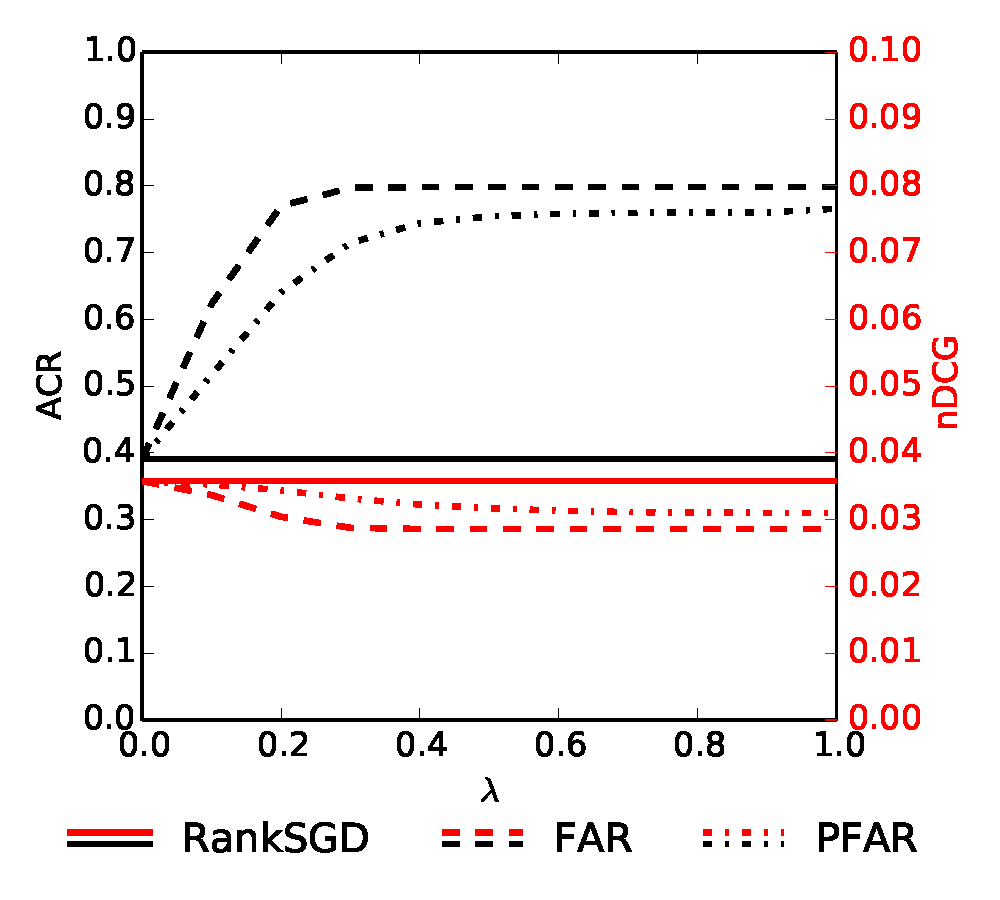
\includegraphics[width=\textwidth]{imgs/far/ranksgd.png}
		\caption{RankSGD \cite{pmlr-v18-jahrer12b}} % subcaption
	\end{subfigure}
	%\vspace{0.2em} % here you can insert horizontal or vertical space
	\begin{subfigure}{0.49\columnwidth} % width of right subfigure
		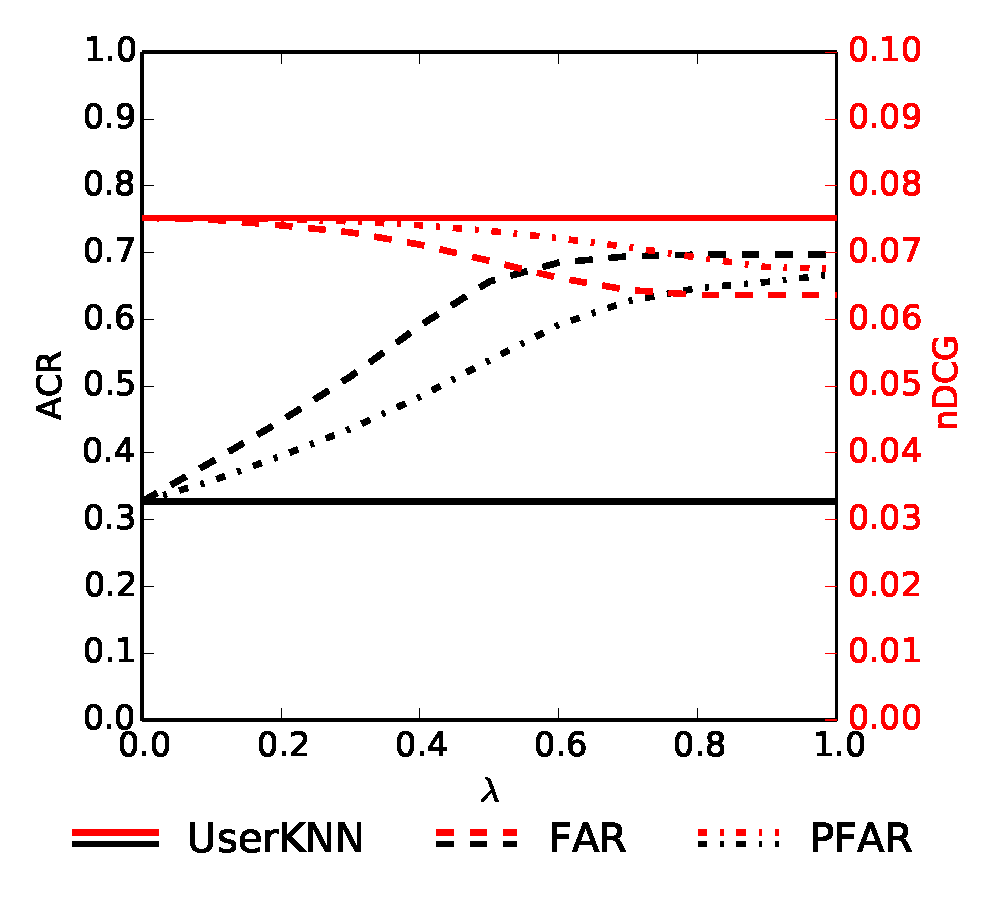
\includegraphics[width=\textwidth]{imgs/far/userknn.png}
		\caption{UserKNN \cite{resnick1997recommender}} % subcaption
	\end{subfigure}
	\begin{subfigure}{0.49\columnwidth} % width of left subfigure
		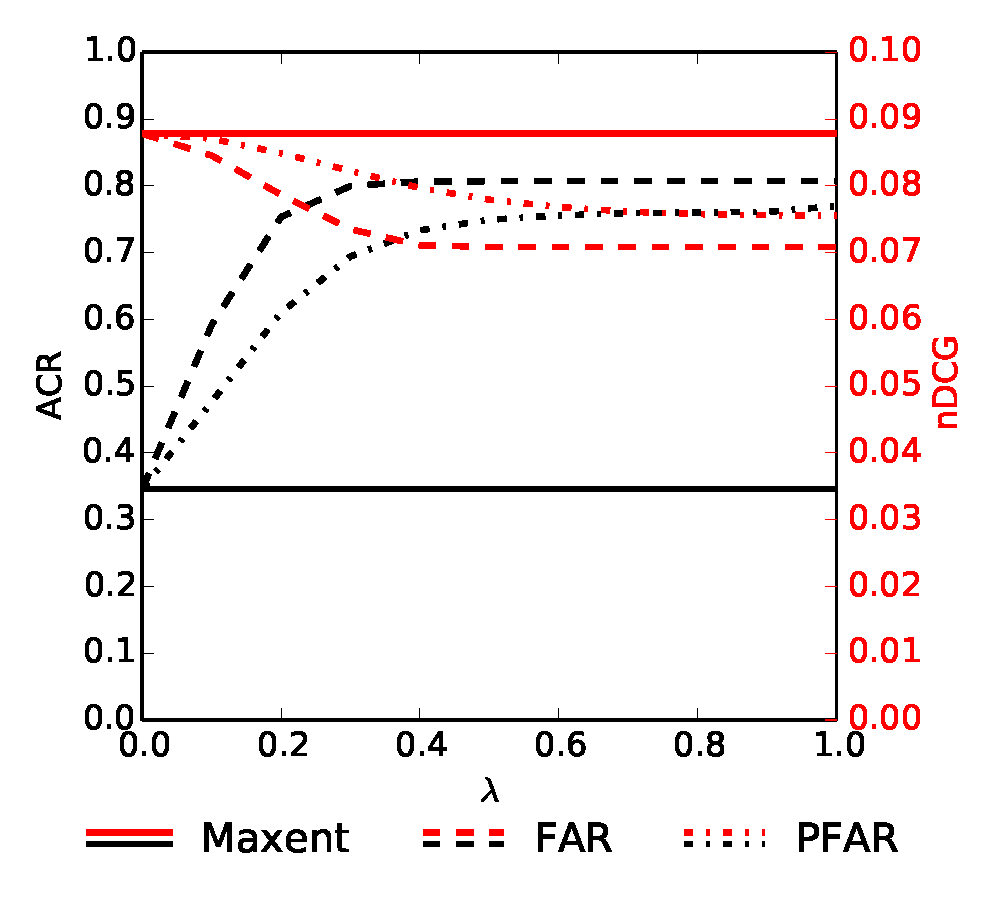
\includegraphics[width=\textwidth]{imgs/far/wrmf.png}
		\caption{WRMF \cite{hu2008collaborative}} % subcaption
	\end{subfigure}
	%\vspace{0.2em} % here you can insert horizontal or vertical space
	\begin{subfigure}{0.49\columnwidth} % width of right subfigure
		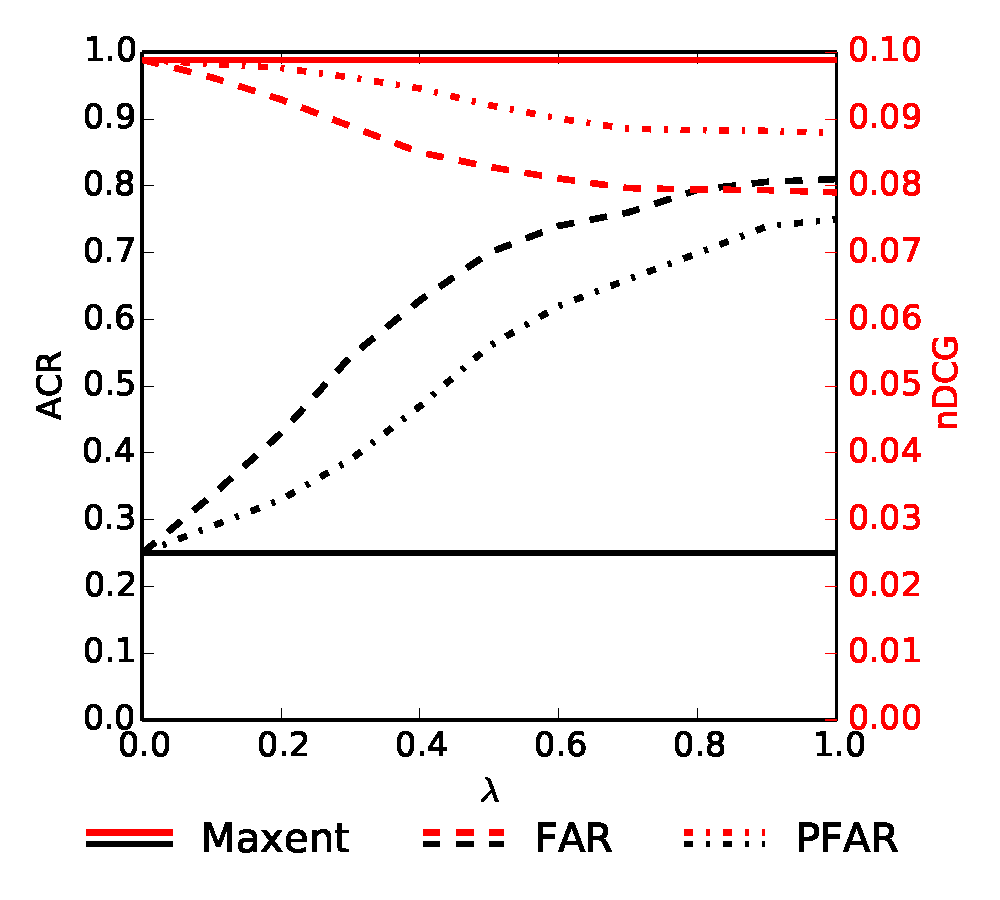
\includegraphics[width=\textwidth]{imgs/far/maxent.png}
		\caption{Maxent \cite{choo2014gather}} % subcaption
	\end{subfigure}
	%\vspace{-0.25cm}
	\caption{Tendencies of ACR and nDCG with increasing $\lambda$.\label{fig:kiva_results}} % caption for whole figure
\end{figure}


Considering the performance of all base recommenders (the solid lines), rankSGD has the lowest accuracy (nDCG = 0.0358); UserKNN comes next with nDCG=0.0752 by finding the nearest neighbors; WRMF performs better than UserKNN by learning the latent factors of lenders and loans (nDCG=0.0878); Maxent obtains the highest nDCG of 0.0988 since Maxent is specially designed for loan recommendation and additional features of loans, \emph{e.g.,} loan sector and geographical coordinates, are utilized. However, accurate recommenders tend to favor items from certain groups, thus resulting in fairness issues.

\paragraph{Effectiveness of the re-ranking algorithms.} By applying our proposed algorithms (when $\lambda\in(0,1)$), all recommenders tend to achieve fairer recommendation results by promoting the loans that belong to less-popular groups, showing the flexibility and effectiveness of our proposed algorithms. Our re-ranking algorithms can be deployed to any base recommender, with the weight of the fairness tunable. The accuracy slightly decreases as $\lambda$ increases, as there is a price to pay for obtaining a fairer system. Take $\lambda=0.1$ for instance, Maxent can obtain a gain of 25.1\% in ACR with a loss of merely 1.6\% in nDCG. Moreover, RankSGD and WRMF converge faster than UserKNN and Maxent with the increase of $\lambda$, indicating that the behavior of our proposed algorithms depends on the initial ranking list to some extent. 

Note that RankSGD has limited ability in learning lenders' preferences, while the results are usually fairer. This is to be expected since accuracy and fairness are conflicting.

\paragraph{Comparison between FAR and PFAR.} The recommendation accuracy of PFAR is higher than FAR, since PFAR limits the amount of loan diversity that the re-ranking imposes, based on the individual tolerance. We can also observe from Figure \ref{fig:kiva_results} that fairness of PFAR is lower, which is consistent with our previous discussion and demonstrates the tradeoff between accuracy and fairness.

%has the highest fairness (ACR = 39.1\%) but the lowest accuracy (nDCG = 0.0358).

% \begin{comment}
% In the first experiment, we plot the tendencies of ACR and nDCG with increasing hyper-parameter $\lambda$, where a larger $\lambda$ means the weight of fairness is larger. Without our proposed re-ranking algorithms (when $\lambda=0$), rankSGD has the highest fairness (ACR = 39.1\%) but the lowest accuracy (nDCG = 0.0358). By utilizing additional content information, \emph{e.g.,} locations of the borrowers, Maxent is the most accurate (nDCG = 0.1) yet unfair (ACR = 25.1\%) recommender. It is because Maxent uses borrower location information as input and learns the biased pattern that lenders are more interested in lending to borrowers from certain regions, which results in an unbalanced recommendation.

% The effectiveness of the proposed re-ranking depends heavily on the quality of the initial ranking list.

% By applying our proposed algorithms (when $\lambda\in(0,1]$), all recommenders tend to achieve fairer recommendation results by promoting the items that belong to less-popular groups. The accuracy slightly decreases as $\lambda$ increases. This is to be expected since accuracy and fairness are conflicting. There is a price to pay for obtaining a fairer system. Interestingly, for Maxent, we could obtain a significant boost in fairness (ACR increases by 71.3\% at $\lambda=0.5$) while accuracy still remains at a high level. The reason may be that Maxent has the ability to discover better items for every borrower group. Therefore, the items may still be attracting for the consumer when promoting the uncovered groups. We also note that the recommendation accuracy is rather low for all base recommenders if we only consider fairness for re-ranking ($\lambda=1$).

% Comparing PFAR to FAR, the recommendation accuracy of PFAR is higher than FAR since PFAR is more personalized and considers the different receptivity of the consumers towards diversified borrower groups. We can also observe from Figure \ref{fig:kiva_results} that the borrower-side fairness of PFAR is lower, which is consistent with our previous discussion and demonstrates the tradeoff between accuracy and fairness.
% \end{comment}



\paragraph{Visualization of the re-ranking results.} We compute the percentage of recommendations for each group with and without the proposed re-ranking algorithms, and study the corresponding allocation distribution. Due to the 4-page limitation, we chose Maxent as an example, and the results are shown in Figure \ref{fig:kiva_num_rec}. Similar trends can be observed for other base recommenders.

(i) The blue bars show the distribution of the base recommender Maxent, \emph{i.e.,} $\lambda=0$. We observe that Maxent focuses on a few major borrower groups, namely Asia and Africa (making up 36.58\% and 27.64\% of total recommendations, respectively), while paying less attention to the others. 

(ii) The ideal fairness is to give each group an equal chance of being recommended. However, accuracy will be significantly downgraded as lenders' preferences are not learned. As a compromise, we find a balance between the two and select $\lambda=0.1$, where the growth rate of ACR per unit nDCG loss is the largest. As illustrated by the green and red bars in Figure \ref{subfig:lambda01}, nDCG still remains at a high level after the re-ranking (nDCG=0.0962 for FAR and nDCG=0.0983 for PFAR), while fairness of the recommendation is significantly improved, as loans belonging to less-popular groups are promoted.

(iii) In Figure \ref{subfig:lambda10}, a larger $\lambda=0.99$ is applied, and the distribution can be even more balanced, while the accuracy is lower.


% To achieve ideal fairness, one would like to give each group an equal chance of being recommended. However, accuracy will be significantly downgraded as lenders' preferences are not learned. As a compromise, we find a balance between the two and achieve a fairer recommendation distribution. We select $\lambda=0.1$, where the rate ACR gain with unit nDCG loss is the largest, and plot the percentage of recommendation of each group of Maxent. Figure \ref{subfig:lambda01} shows that Maxent focuses on a few major borrower groups, namely Asia and Africa (accounting for 36.58\% and 27.64\% of total recommendations respectively), while paying less attention to the others. After the re-ranking, nDCG still remains at a high level (nDCG=0.0962 for FAR and nDCG=0.0988 for PFAR), while fairness of the recommendation is significantly improved, as loans belong to less-popular groups are promoted. In Figure \ref{subfig:lambda10}, a larger $\lambda=0.99$ is applied, the distribution can be even more balanced, while the accuracy is lower.

% Next, we compute the number of recommendations for each provider group, as shown in Figure~\ref{fig:kiva_num_rec}. The weight $\lambda$ is chosen at the maximum unit growth rate of ACR with respect to nDCG. For all base recommenders, the recommendation distribution is unbalanced. Especially for Maxent, almost all recommendations occur in Asia and Africa, accounting for 55.77\% and 34.71\% of total recommendations respectively, while other regions barely get recommended.

% able~\ref{tab:inventory} shows the prevalence of each region in the pseudo-item loan inventory, and demonstrates there is certainly over- and under- representation in the results of all base recommenders. For Oceania, we expect 1/15 loan recommendation as Africa if the recommendation lists were proportional to the inventory. However, Oceania almost has no recommended loans. For PFAR and PFAR, with a reasonable decline in nDCG, regions like Eastern Europe and Oceania are increasingly recommended and the distribution is more balanced.

% demonstrates that the unbalance is not caused by the number of loans each region owns (\emph{i.e.,} the inventory of each region), since the number of recommendations generated by WRMF is not proportional to the inventory.



\begin{figure}
\centering
\begin{subfigure}{0.495\columnwidth}
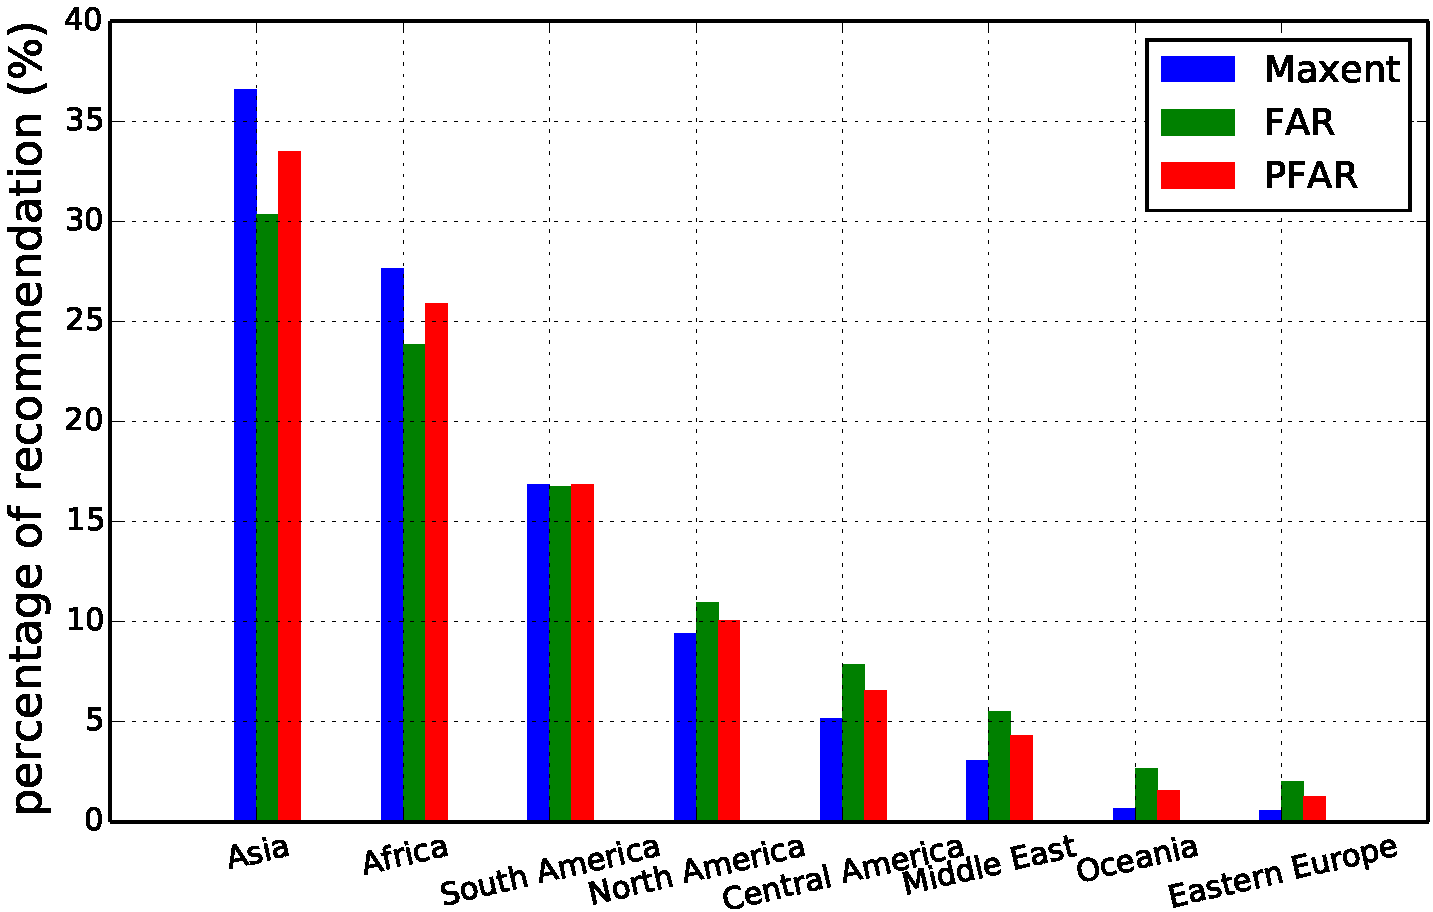
\includegraphics[width=\textwidth]{imgs/far/maxent-lambda01.png}
\caption{$\lambda=0.1$, $\text{nDCG}_{\text{FAR}}=0.0962$,\;\;\;\;\;\; $\text{nDCG}_{\text{PFAR}}=0.0983$. \label{subfig:lambda01}}
\end{subfigure}
\begin{subfigure}{0.495\columnwidth}
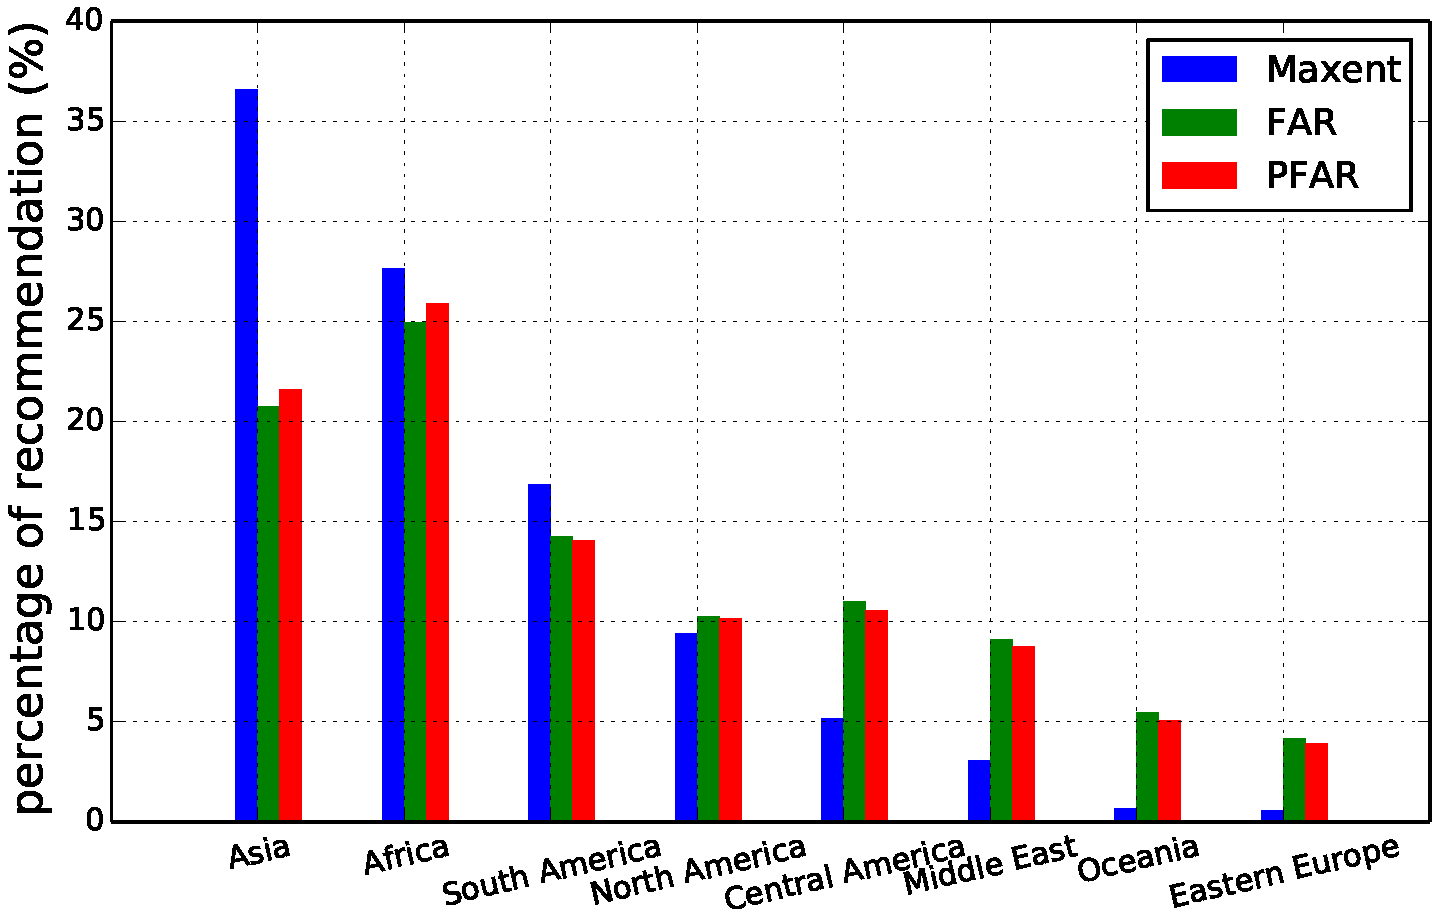
\includegraphics[width=\textwidth]{imgs/far/maxent-lambda10.png}
\caption{$\lambda=0.99$,  $\text{nDCG}_{\text{FAR}}=0.0709$,\;\;\;\;\; $\text{nDCG}_{\text{PFAR}}=0.0756$.\label{subfig:lambda10}}
\end{subfigure}
%\vspace{-0.25cm}
\caption{Recommendation percentage of each region. The blue bars show the results of the base recommender ($\lambda=0$). The green and red bars represent the results of FAR and PFAR, respectively.\label{fig:kiva_num_rec}}
\end{figure}
% The blue bars show the results of the base recommender ($\lambda=0$). The green and red bars represent the results of FAR and PFAR, respectively.


\subsubsection{\textbf{Conclusion and Future Work}}\label{sect:conclusion}
In this work, we proposed a personalized fairness-aware re-ranking algorithm for microlending that can balance accuracy and fairness. We increase the coverage rate of borrowers' regions for Kiva.org to achieve borrower-side fairness, and we show that our algorithm can do so with minimal loss in ranking accuracy. In addition, our algorithm includes lender-specific weights that can be used to personalize the degree of loan diversity.

% In the future, we will consider the position bias into the fairness-aware recommendation for microlending. As discussed in this paper, the recommendation for microlending is moved forward by considering the coverage rate of borrowers and the lenders' diversity tolerance. However, the top positions are generally more valuable than the bottom ones \cite{robertson1977probability}. We plan to make a further assumption that the chance of exposure for an item depends on its position in ranking. Thus, incorporating such position bias into the re-ranking criteria for microlending is promising.

% In the future, we will study a number of variants of our algorithms presented here. We plan to explore different methods for computing personalized diversity tolerance factors, especially to solve the cold-start problem in the current algorithm. We also plan to examine variants of the re-ranking algorithm to take into account the size of each provider group's inventory. 

FAR/PFAR is extremely strict in its requirement that each possible provider group appears at least once at the top of the list. Therefore, another variant to consider is one that can adjust the accuracy/fairness tradeoff in a dynamic way as items are ranked, valuing accuracy more at the top of the list and provider-side fairness more at the bottom of the list.

Finally, we note that, in real-world recommendation applications, managing the tradeoff between accuracy and coverage of provider groups is not a single-shot process. Rather it is an online process, where a current lack of coverage can be compensated for at a later time, and where results are evaluated temporally. This would require making the algorithm sensitive to historical patterns of coverage, rather than just the results obtained in the current list. We intend to explore this type of algorithm design and evaluation in our future work.

This project currently is an on-going project and we intend to develop a method using probabilistic serial allocation and submit it to the ACM Conference Series on Recommender Systems 2021.
\subsection{Opportunistic Multi-aspect Fairness through Personalized Re-ranking}

% Recommender systems are designed to assist users to find items of interest. Such systems model users' historical behaviors and generate personalized recommendations tailored to users' interests or needs. Recent research has identified a key limitation in a user-focused approach to recommender systems development, namely that it ignores multistakeholder aspects of the systems in which recommendation is embedded\cite{abdollahpourimulti2020}.

In this section we focus on the \textit{provider fairness} again where it concerns the impact of recommendation delivery on the providers of items being recommended and the questions of fair treatment that may arise\cite{burke2017multisided}.

Recent research has sought to alleviate this concern, including the re-ranking method in the previous section, using a variety of approaches. See, for example, \cite{yao2017beyond,burke2018balanced,ekstrand2018exploring,liu2019personalized,kamishima2016model,beutel2019fairness}. What all of these approaches share is that they focus on a \emph{single dimension} over which fairness is sought: a single protected group among the providers, and except for \cite{liu2019personalized}, they do not take user preferences in item features into account.

% The problem of promoting provider fairness while maintaining recommendation accuracy can be generally characterized as a multi-objective optimization problem. If optimal fairness and optimal recommendation accuracy could be achieved simultaneously, there would be no need for research in this area. However, optimizing recommendation accuracy often comes at the expense of provider fairness, due to various biases present in recommender systems, including popularity bias \cite{celma2008hits,lee2014fairness}, and user-base composition \cite{lin2019crank, yao2017beyond}. Research in provider fairness is therefore generally concerned with improving the tradeoff between fairness and accuracy, or in other words, increasing the amount of fairness that can be gained for a given degree of accuracy loss.

% Rather than look for improvements through global optimization as in \cite{yao2017beyond},

Our work in this paper extends the FAR/PFAR approach discussed in the previous section  which was seeking to improve the accuracy / fairness tradeoff through increased \textit{personalization}. Namely, can we tailor the type and degree of optimization specific to each user's tastes and preferences and therefore improve accuracy? We label this approach \textit{opportunistic} because we view each user as presenting a particular type of opportunity to increase recommendation fairness and try to make the most of each. In particular, we seek to identify the particular dimensions along which a user might be open to result diversification that improves fairness and thereby enable multiple fairness concerns to be addressed at once.


\begin{table}[htb]
    \begin{tabular}{|c|c|c|c|c|}
    \hline
        $user_{1}$ & $F_{1}$:Region & $F_{2}$:Gender & $F_{3}$:Sector & $F_{4}$:Amount \\
    \hline
        $item_{1}$ & Africa & Female & Agriculture & \$0-\$500\\
    \hline
        $item_{2}$ & Africa & Female & Health & \$0-\$500\\
    \hline
        $item_{3}$ & Africa & Female & Clothing & \$0-\$500 \\
    \hline
    \end{tabular}
    \caption{Profile of $user_{1}$}
    \label{table:user_profile}
\end{table}
% \vspace{-7mm}

As an example, in the context of loan recommendation, suppose user $u$ prefers to lend her money to women in Kenya but she does not have a strong preference for a loan's purpose or economic sector. This user's profile might appear as in Table \ref{table:user_profile}. While the user might not respond well to loans in other countries, we can consider her open-mindedness regarding the Sector feature as an opportunity to increase fairness in this area. For the sake of example, assume loans from the Education and Conflict Zones sectors are historically underfunded in Kenya, so the loans in these sectors are identified as protected. Consider the recommendation results in Table \ref{table_user_recoms}. The first two recommendations ($r_1 and r_2$) increase fairness across only the Sector feature by promoting items from underfunded sectors while honoring the user's preference to lend money to Kenyan women. On the other hand, loan $r_3$ might not be an effective recommendation for this user since it diversifies on the wrong dimensions, although it might still be promoting protected items. In other words, we want to promote fairness concerns when the user's profile indicates receptivity and be cautious otherwise.

% \vspace{-1mm}
\begin{table}[tbh]\centering
    \begin{tabular}{|c|c|c|c|c|}
    \hline
        $user_{1}$ & $F_{1}$:Region & $F_{2}$:Gender & $F_{3}$:Sector & $F_{4}$:Amount \\
    \hline
        $r_{1}$ & Africa & Female & Conflict Zones & \$0-\$500\\
    \hline
        $r_{2}$ & Africa & Female & Education & \$0-\$500\\
    \hline \rowcolor[gray]{0.7}
        $r_{3}$ & Asia & Male & Livestock & \$500-\$700\\
    \hline
    \end{tabular}
    \caption{Recommendations for $user_{1}$}
    \label{table_user_recoms}
\end{table}

% In the example above, $user_{1}$ doesn't have a strong preference for the loan sector. 
% So, in the final recommendations below, we prioritize loans from Education and Conflict Zones, since we know they are under-funded in Kenya. In the table below the first and second recommendations are generated using personalized diversity while considering fairness constraints and the last recommendation is uniformly diversified across different dimensions ignoring users' tolerance for diversity and the fairness of a system.

This paper addresses the following research questions:
\begin{description}
    \item [RQ1:] Do users exhibit different patterns of preference across fairness dimensions?
    \item [RQ2:] Can these patterns be exploited to improve the recommendation fairness / accuracy tradeoff using re-ranking?
\end{description}

\subsubsection{\textbf{Background}}
\label{sec:backgroundd}

This line of research has much in common with work that seeks to enhance diversity in recommendation \cite{zhang2008MonotonyDiv, vargas2011rankRelDiv, carbonell1998use, eskandanian2017clustering}. However, the key differences have to do with the concerns being addressed and, accordingly, the way in which success is measured. Usually when diversity is invoked as a desirable property of a recommender system, it is in the service of some user-oriented goal. Diverse recommendations can help a system cope with a diverse range of user intents and contexts. For example, a restaurant recommender might know that a user sometimes goes to family-style pizzerias 70\% of the time and fancy French restaurants 30\% of the time. Rather than present just pizzerias in a recommendation list, even though that is likely to be the right answer statistically, it might be better to include one or two fine dining establishments on the list, just in case the user is looking for a ``date night'' recommendation this time around. 

Typical measures of diversity such as intra-list distance, for example \cite{Ziegler:2005:IRL:1060745.1060754}, therefore measure the difference among items in each user's list, without regard to what items they are. Diversity as a fairness concern seeks varied outputs for a completely different reason, namely to increase the prevalence of items from under-represented providers, and measures outcomes relatively to those providers specifically. We will distinguish between these sense of diversity by using the term \textit{list diversity} to refer to the user-centered objective and \textit{fairness-promoting diversity} to the provider-centered objective, our main concern in this paper.

Another related definition of diversity is what is called \textit{aggregate diversity} or catalog coverage. The question here is whether the recommender is presenting all of the available items in the catalog. This can be seen as a minimal form of fairness where the frequency of appearance is not considered, just that an item is recommended at least once, and we do not differentiate between different items or different providers~\cite{adomavicius2011improving}.

As noted above, most work in recommendation fairness, and machine learning fairness more generally, simplifies the problem of fairness-enhancement by concentrating on a single (usually binary) distinction between a protected group and an unprotected group. This is an excellent starting point and admits of tractable mathematical formulations. However, this approach is not a good match to real-world applications, where there are likely to be multiple fairness concerns related to multiple dimensions of identity \cite{kearns2019empirical}.

From the user perspective, the effect of these considerations is more or less the same: the recommender produces recommendations that are more diverse than would be found based on personalization considerations alone. It is only in looking at the recommendations in aggregate and considering the system's objectives that different diversity methods can be readily distinguished.

% The choice of which type of  in which the items vary  It is only in looking at the recommendations in aggregate and considering the system's objectives that they can be readily distinguished. 

\subsubsection{\textbf{Problem formulation}}
\hfill

Given a set of users $\mathcal U=\{u_1,\ldots,u_n\}$, a set of items $\mathcal V=\{v_1,\ldots,v_m\}$, and initial ranking lists $R(u)$ for users $u\in \mathcal U$, our task is to re-rank $R(u)$ and generate a list of $k$ distinct items $S(u)$ that is both accurate and fair similar to \cite{liu2019personalized}'s goal.

We will further assume that each item $v_i\in\mathcal V$ is represented by a $d$-dimensional feature vector $\vec{\phi}_i = \langle f_{i1},\ldots,f_{id}\rangle$ over a set of categorical features $F = \{F_1, F_2, \ldots, F_d\}$. Each dimension $F_j$ can be viewed as a set of categorical values or labels and so for an item $v_i$, its feature vector $\phi_i$ contains $f_{ij} \in F_j$ for each feature $F_j$. We will use the notation $c_j = |F_j|$ to refer to the cardinality of the feature $F_{j}$.

As an example, suppose that our set of items are loans and users are our potential lenders. Suppose that each loan is characterized by two features: geographical region and economic sector. Thus, $F = \{\mathrm{Region}, \mathrm{Sector} \}$, and $d = 2$. Suppose that we have 5 geographical regions and 7 economic sectors. For example:  $\mathrm{Region} = F_1 = \{\mbox{Africa}, \mbox{Asia}, \mbox{Americas}, \ldots\}$ and $\mathrm{Sector} = F_2 = \{\mathrm{Agriculture}, \mathrm{Housing}, \mathrm{Education}, \mathrm{Conflict Zones}, \ldots\}$. If a particular loan $v_i$ is sought in the agriculture sector in Africa, we would say $\vec{\phi}_i = \langle \mathrm{Africa}, \mathrm{Agriculture} \rangle = \langle f_{i1}, f_{i2} \rangle$.

%We will further assume that each item $v_i\in\mathcal V$ has an associated feature vector $\vec{x}_i$ of dimension $\ell$ containing features that describe the item: $\vec{x}_i = \langle f_{i1},\ldots,f_{i\ell}\rangle$. The $f_{ij}$ values are elements of categorical ranges for each feature dimension: $f_{ij} \in F_j$. We will use the notation $c_i = |F_i|$ to refer to the cardinality of these feature categorizations and $F_{jk}$ to refer to specific values in these dimensions. We will use the vector $\mathcal X$ and its elements $X_i$ to refer to the labels associated with each feature dimension. 

%Therefore, suppose have a set of items that are loans a user might lend money to and these loans are characterized by geographical region and economic sector. We would say that $X = \langle \mathrm{Region}, \mathrm{Sector} \rangle$, $\ell = 2$. Suppose that we have 5 geographical regions and 7 economic sectors. $F_1 = \{\mbox{Africa}, \mbox{Asia}, \ldots\}$, $F_2 = \{\mathrm{Agriculture}, \mathrm{Housing}, \ldots\}$. If a particular loan $v_j$ is sought in the agriculture sector in Africa, we would say $\vec{x}_j = \langle \mathrm{Africa}, \mathrm{Agriculture} \rangle = \langle f_{j1}, f_{j2} \rangle = \langle F_{11}, F_{21} \rangle.$

A protected class, within some $F_j$ feature, consists of a set of values $F_j' \subset F_j$ that are considered protected and for which fairness is sought. There may be multiple fairness dimensions of concern, we define the protected dimensions  $F'$ as the subset of $F$ that contain such protected values. For example, if Education and Conflict Zone loans are relatively underfunded, then in the Sector feature, these two specific values form the protected group $F'$. 
%we define the protected dimensions

\paragraph{\textbf{Personalized diversity}}

Studies have shown that users generally prefer more recommendation results they perceive as diverse \cite{hu2011enhancing}. This suggests that the opportunity for fairness-enhancing diversification exists and may come at minimal cost in terms of user experience. However, users differ in the variety that they seek in recommendations~\cite{tintarev2013adapting}. Some recommendation research has sought to capitalize on these differences in improving diversity \cite{eskandanianuser_2016}. Here we aim to do the same in a more fine-grained way, consider each user's interest in diversity across multiple features.

Figure \ref{fig:uniform_vs_personalized_div} gives a schematic depiction of this distinction. In this example, each item has a color and a shape feature. A user profile, shown at the top, consists of squares of different colors. Clearly, this user has a strong interest in squares and cares less about what color they are. A recommender that prioritizes triangles and circles as a protected group as well as greenish/yellowish hues might deliver recommendations as shown in the second row. These will likely not be accepted as they deviate too much from the characteristics preferred by the user. A better approach would be to diversify only in (the dimensions/values of) color, retaining the aspect of the items that the user apparently prefers.

\begin{figure}[tbh!]
    \begin{center}
        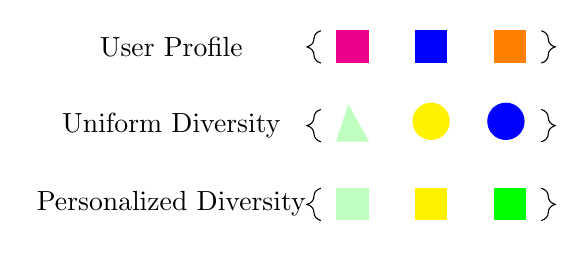
\begin{tikzpicture}
        
        % user profile
        \node at (-5.5, 3.2) {User Profile};
        \draw [magenta, fill] (-3, 3) rectangle (-3.4, 3.4);
        \draw [blue, fill] (-2, 3) rectangle (-2.4, 3.4);
        \draw [orange, fill] (-1, 3) rectangle (-1.4, 3.4);
        \draw [decorate,decoration={brace,amplitude=5pt},xshift=-0.5cm,yshift=0pt] (-3.1,2.99) -- (-3.1,3.4) node [black,midway,xshift=-1cm] {};
        % mirror=-0.5cm,
        \draw [decorate,decoration={brace,amplitude=5pt},yshift=0pt] (-0.8,3.4) -- (-0.8,2.99) node [black,midway,xshift=-1cm] {};
        
        % diversifying uniformly
        \node at (-5.5, 2.2) {Uniform Diversity};
        \draw [green!25, fill] (-3.4, 2) -- (-3, 2) -- (-3.25, 2.45) -- cycle;
        \draw [yellow, fill] (-2.2, 2.25) circle [radius=0.23];
        \draw [blue, fill] (-1.25, 2.25) circle [radius=0.23];
         \draw [decorate,decoration={brace,amplitude=5pt},xshift=-0.5cm,yshift=0pt] (-3.1,1.99) -- (-3.1,2.4) node [black,midway,xshift=-1cm] {};
        % mirror=-0.5cm,
        \draw [decorate,decoration={brace,amplitude=5pt},yshift=0pt] (-0.8,2.4) -- (-0.8,1.99) node [black,midway,xshift=-1cm] {};
        
        
        % personalized diversity
        \node at (-5.5, 1.2) {Personalized Diversity};
        \draw [green!25, fill] (-3.4, 1) rectangle (-3, 1.4);
        \draw [yellow, fill] (-2.4, 1) rectangle (-2, 1.4);
        \draw [green, fill] (-1.4, 1) rectangle (-1, 1.4);
        \draw [decorate,decoration={brace,amplitude=5pt},xshift=-0.5cm,yshift=0pt] (-3.1,0.99) -- (-3.1,1.4) node [black,midway,xshift=-1cm] {};
        % mirror=-0.5cm,
        \draw [decorate,decoration={brace,amplitude=5pt},yshift=0pt] (-0.8,1.4) -- (-0.8,0.99) node [black,midway,xshift=-1cm] {};
        
        \end{tikzpicture}
    \end{center}
    % \includegraphics{}
    \caption{Uniform vs Personalized Diversity }
    \label{fig:uniform_vs_personalized_div}
\end{figure}
% \vspace{0.4mm}
% \begin{figure}[h!]
%     \centering
%     \includegraphics[width=8cm]{plots_camera/uniform_personalized_div.png}
%     \caption{Uniform vs Personalized Diversity}
%     \label{fig:uniform_vs_personalized_div}
% \end{figure}


% Liu et al. \cite{liu2018personalizing,liu2019personalized} 
In the previous section, we introduced the concept of recommendation re-ranking using a quantity $\tau_u$, a user-specific measure of interest in diversity, based on information entropy \cite{liu2018personalizing,liu2019personalized}. Here we extend this definition to take into account multiple item features while seeking fairness within each feature's dimensions. Instead of a single user-specific $\tau_u$, the $\vec{\tau}_u$ vector will represent the user's level of tolerance for diversity across the feature space (such as the user in the above example having more tolerance for diversity in the ``color'' feature and less in the ``shape'' feature). Specifically,

\begin{equation}
\vec{\tau}_u(F_{j})\buildrel\triangle\over=-\sum_{f \in F_j} P(f|u)\log P(f|u),
\label{eq:tau}
\end{equation}

where $P(f|u)$ is computed as the fraction of items in the user's profile that have the feature value $f$. This can be interpreted as the user's likelihood of liking items with that value. The higher the entropy value is for a user on a feature, the higher her tolerance to see diversity within that feature. For example, the user in Table~\ref{table:user_profile} would have low entropy for Region and Gender, but higher entropy for Sector.

This vector of values, therefore, quantifies the relative opportunities for providing diverse results to users. As we show in Section 5.4, these values vary widely across different features and different users, motivating a recommendation techniques that is sensitive to these individual differences. 

\paragraph{\textbf{Recommendation re-ranking}}

Re-ranking is a common technique for enhancing the non-accuracy properties of recommender systems output. It provides a relatively simple framework for augmenting an existing recommender system with concerns that are not part of its design. Generally speaking, a re-ranker is a function that maps a ranked list $R(u)$ of size $k$ (e.g., a ranked recommendation list) and produces a new list $S(u)$ of size $k'$ where $k'<= k$ and where all items are drawn from the original list: $\forall{i}: i \in S(u) ~\mathit{iff} i\in R(u)$. The loss of ranking accuracy in doing so is thereby limited by the size $k$; no item in $S(u)$ can be worse than what the original recommendation placed at rank $k$. 

Re-ranking algorithms of this type were introduced in information retrieval for enhancing user-oriented diversity. The \textit{Maximum Marginal Relevance} method as proposed in \cite{carbonell1998use} measures for each user, the dissimilarity between a query and the items in her retrieved results. This method intends to combine query relevance and list diversity using a greedy list accumulation algorithm. The algorithm builds the output list $S$ one item at a time. 

At each point in time, it scores potential new items by a combination of their relevance (as computed in the initial retrieval step) and their differences from the current list (novelty), computed by identifying the item $j \in S$ that is most similar to the new item.

In our context, we will assume that we have some function \textit{sim} that computes similarity between two items $i, j$ and that our recommender system returns a relevance score of \textit{rec(v,u)} for a user $u$ and item $v$. We can then define the MMR-based scoring function:

\begin{equation}
    \mathit{OFAiR}(u,v,R,S)\buildrel\triangle\over= \arg\max_{v \in R \setminus S} [\lambda  (\mathit{rec}(v,u) - (1 - \lambda) \sum_{v' \in S} \mathit{sim}(v,v')]
\label{eq:mmr}
\end{equation}

Effectively, the algorithm, at each point, finds the next item to include by incorporating the original ranking (as encapsulated in the recommendation score), but penalizes that score when the proposed item is highly similar to the items already added.

There is a subtle difference between the MMR formulation here and its original specification. When scoring a new item to decide whether to add it to the re-ranked list, MMR chooses the most similar item -- this is the ``marginal'' part of the algorithm. Our formulation calculates the summation of similarities between the target item and all the other items in the re-ranked list. We can think of this as identifying the item with maximum aggregate difference from the existing list. We will explain later how this change is appropriate in a fairness context.

\textit{eXplicit Query Aspect Diversification} method proposes another formulation to enhance diversity. Although, this method has a similar goal to MMR, it enhances diversity with respect to specific aspects of an item \cite{santos2015search}. The diversity objective relative to a particular aspect (e.g., feature, topic, or category) is considered satisfied if one item containing that aspect is added to the result list. In context of recommendations, we can express this ranking score as follows:

\begin{equation}
    \mathit{xQuAD}(u,v,R,S)\buildrel\triangle\over= \arg\max_{v \in R \setminus S} [\lambda  (\mathit{rec}(v,u) + (1 - \lambda) \max_{v' \in S} \mathds{1}_{\vec{v} \cap \Vec{v'} = \emptyset}],
\label{eq:xquad}
\end{equation}
\noindent where $x_v$ represents the set of aspects present in item $v$. In effect, this algorithm boosts the rank of items that, when added to the list so far, bring in new aspects -- features that have not yet appeared in the list. 

In FAR/PFAR algorithms in the previous section \cite{liu2018personalizing,liu2019personalized}, we proposed two extensions to xQuAD. The first \textit{FAR} (Fairness-Aware Reranking) applied the formalism using aspects of an item defined over a fairness-relevant feature. In this configuration, the algorithm boosts the scores of items from protected groups when no such item has yet been added to the list. Once the group is represented, the boosting disappears. This can be seen as an implementation of the ``Rooney rule'' \cite{kleinberg2018selection} that ensures minimum representation for protected groups. The second variant \textit{PFAR} adds personalization to this process. Using the $\tau_u$ information entropy measure described above, the fairness-boosting term is modulated so that users with more diverse profiles (who have a high diversity tolerance/higher entropy) are presented with results containing more fairness-enhancing diversity.

In particular, the scoring function of PFAR is composed of a personalization score $\mathit{rec}(v,u)$ and a personalized fairness score. PFAR simply assumes only one sensitive feature need to be considered. Suppose the given sensitive feature dimension is $F_a$, then the scoring function is defined by

\begin{equation}
    \mathit{PFAR}(u,v,R,S)\buildrel\triangle\over= \arg\max_{v \in R \setminus S}[\lambda\mathit{rec}(v,u) + (1-\lambda)\tau_u \min_{v' \in S} \mathds{1}_{v_{a} \neq v'_{a}}],
\end{equation}

where $v_{a}$ is the a-th element of the feature vector $\vec{v}$.
Note that PFAR inherits the limitation of xQuAD that it assumes binary inclusion as a sufficient definition of fairness and it is therefore difficult to tune it to improve the representation of protected groups in a proportional way. 
\newpage

\subsubsection{\textbf{Opportunistic fairness}}
\hfill

We are now ready to describe \textit{OFAiR} (\textbf{O}pportunistic \textbf{F}airness-\textbf{A}ware \textbf{R}eranking), which incorporates personalization at the feature level into the re-ranking process and also allows fine-grained control of protected group promotion by using per-feature weights. 

As discussed above, we can represent the variation in a user's profile across all features through the vector $\vec{\tau}_u$, calculated using information entropy. However, because these weights are feature-specific, we cannot incorporate them as a single multiplier as found in PFAR. Also, because we are interested in fine-grained control over the proportions of protected group items in recommendation lists, the xQuAD formula with its binary inclusion metric is not appropriate. So, our alternative in OFAiR applies the MMR approach by penalizing item similarity, but we build the feature significance into the similarity metric itself. We want to add items to the recommendation list if they add to the representation of protected groups in the recommendation list and if they differ from the items on the list in areas of high diversity tolerance for the user. To achieve this effect, we multiply together the user-specific tolerance weight for each feature and a weight associated with a feature's protected / unprotected class. 

We use weighted cosine similarity to allow the similarity between two items to be controlled by weights associated with each dimension. Because the weights actually vary by value, not just by dimension, and we can only pass a single weight vector to the weighted cosine similarity function, we convert the feature vector $\vec{\phi}$ to a smoothed binary vector of dummy variables $b_i$ with one dimension for each possible feature value. The smoothing operation means that instead of missing values being represented by zero, they have a small value $\epsilon = 2.2e^{-16}$. The user tolerance weights are correspondingly expanded in dimension to match: $\vec{\tau}_u \rightarrow \vec{\gamma}_u$. 

Let $\vec{a} \circ \vec{b}$ represent the element-wise (Hadamard) product between two vectors $a$ and $b$. Let $W(f')$ be a function that returns the weight of a particular binary feature value $f'$. This value will be small for unprotected values and larger for protected values as described below. For all items, we derive a weight vector $\vec{w}$ where the elements $w_j = W(f'_{j})$. Let $\vec{z_{u}}$ be the product, which combines the two types of weights. %, normalized so that the values sum to 1.
\begin{equation}
\vec{z}_u = \vec{\gamma}_u \circ W(F')
\end{equation}
The entries $z_{uj}$ represent the weight assigned to user $u$ for the $j$th dummy (smoothed binary) feature, combining both individual diversity tolerance and the system's fairness objective.

The weighted cosine metric applies weights to the terms of the cosine computation:
\begin{equation}
    \mathit{wcos}(\vec{b}, \vec{b}', z_u)\buildrel\triangle\over= \sum_{j}^{|F|}{z_{uj} b_j \times b'_j} \frac{1} {\sqrt{\sum_{j} {z_{uj} b^2_j}} \times \sqrt{\sum_{j}{z_{uj} 
    b'^2_j}}}
\end{equation}

Two items are similar under this calculation if their values on many dimensions are the same and those dimensions are ones where the user profile has high entropy / variation and where their associated weight is high. 

Recall that the similarity calculation in MMR is used to penalize items that would be redundant with what is already in the recommendation list. So, the higher the similarities are, the higher the penalty. Therefore, we will want a weighting scheme where protected items are weighted high: their similarity is more important to the system.

This weighting scheme interacts with our aggregate difference alteration of the MMR algorithm noted above. By definition, protected items will be a small subset of the recommended items. Therefore, protected items will always differ from the list in aggregate. Also, the features in the recommendation list are likely to reproduce the consistencies in the user profile that represent lower tolerance for diversity. Weighting the protected features more highly helps promote diversity on those dimensions while keeping the other dimensions less diverse.

Various schemes for the weighting function were considered in our experimentation. In this paper, we report on a simple scheme where protected features receive a fixed high weight $\alpha$ and unprotected features a fixed low weight $\alpha/100$. In our experiments, the results were not sensitive to the magnitude of these values as long as protected features have a lower weighting. Additional exploration of feature weighting will be considered in future work. 


\subsubsection{\textbf{Experiments}}\label{sect:expp}
\paragraph{\textbf{Evaluation Metrics}}
The accuracy of the following methods was evaluated based on Precision, Recall, normalized discounted cumulative gain (nDCG), and to calculate their feature-based diversity both intra-list distance (ILD) and entropy of the recommendation lists were used. The fairness of lists was evaluated based on protected group exposure, which measures the fraction of the recommendation list that consists of protected group items. This value is related to the fairness concept of ``statistical parity,'' measured relative to items' level of promotion within the recommender system. Because list lengths are fixed (10 in our case), the exposure of unprotected items is just one minus the protected group exposure.

\paragraph{\textbf{Dataset}}
We test our model on two datasets. The first is The Movies Dataset, which was obtained from the Kaggle website and contains the metadata of 45,000 movies listed in the Full MovieLens Dataset \footnote{https://grouplens.org/datasets/movielens} which were released on or before July 2017. Although movies are not a domain to which important fairness concerns are typically applied, we use this dataset as a well-known example with a rich set of provider-side features. The dataset contains 26 million ratings from 270,000 users for all 45,000 movies. Ratings are on a scale of 1-5. Each movie contains a set of features from which the following were used in this project: genres, original language, release date, revenue, run-time, popularity, production countries and spoken language. A sample of this dataset was extracted which contained the 559,070 ratings from 6,000 users on 14,623 items (density of 0.63\%).

All the features were transformed into categorical variables. If the movie's popularity is greater than the average popularity, we tag the movie as popular and unpopular otherwise. We transform the revenue and run-time in the same way as well. The release date is bucketed into old and new if the movie's release date is before or after 1990 \cite{kamishima2016model}. All the categorical features were transformed into dummy variables, resulting in a total of 323 binary features.

For the purposes of exposition, we selected two features in each dataset along which to identify protected features, although the OFAiR algorithm supports any number of sensitive features. In the Movies Dataset, we identified the following protected classes within each feature: ``unpopular'' (popularity), ``lower revenue'' (revenue) , ``longer'' (running time), ``before 1990'' (release date), some genres and movies the were produced in some non-US countries. More specifically, in our experiments, within genre and production country features we chose ``Horror'', ``Music'', ``Mystery'', ``History'' (genres) and ``CA'', ``ES'', ``DE'', ``HK'' (countries) to be the protected group. These feature values were chosen because they represented a minority within each feature, and so are good exemplars for demonstrating the capabilities of our algorithm.

Our algorithms are also evaluated on a proprietary dataset obtained from Kiva.org, including all lending transactions over an 12-month period. Initially, there were 1,084,521 transactions involving 122,464 loans and 207,875 Kiva users. Of these loans, we found that 116,650 were funded, that is they received their full funding amount from Kiva users by the 30-day deadline imposed by the site. We selected only the funded loans for analysis. Each loan is specified by features including borrower's name/id, gender, borrower's country, loan purpose, funded date, posted date, loan amount, loan sector, and geographical coordinates. 
To reduce the feature space, and to solve the multicollinearity problem, highly correlated features were removed. The percentage funding rate (PFR) was added as a new feature, computed as follows:
% \vspace{-0.1cm}
\begin{equation}
 \mbox{\textit{PFR}} =  \frac{1}{\mbox{\textit{{\#} days to fund}}} * 100 
\end{equation}

The percentage funding rate captures the speed at which a loan goes from being introduced in the system to being fully funded.\footnote{Loans not fully funded within 30 days are dropped from the system and the money raised is returned to lenders.} For example, a loan with PFR of 25\% is accumulating a quarter of its needed capital each day. After preparing the data, the final features for each loan reduced to borrower's gender, borrower's country, loan purpose, loan amount (binned to 10 equal-sized buckets), and loan's percentage funding rate. We found that this dataset was highly sparse (density = $4.2e^{-5}$) and could not support effective collaborative recommendation, because a loan can only attract a limited amount of support (up to that needed for its funding). There are no ``blockbuster'' loans with thousands of lenders.

To generate a denser dataset with greater potential for user profile overlap, we applied a content-based technique creating \textit{pseudo-items} that represent groups of items with shared features. We applied agglomerative hierarchical clustering \cite{rokach2005clustering} using the features of borrower gender, borrower country, loan purpose, loan amount (binned to 10 equal-sized buckets), and percentage funding rate (4 equal-sized buckets). We chose the cluster with the highest Silhouette Coefficient \cite{rousseeuw1987silhouettes} of around 0.69 which indicates a reasonable cohesion of the clusters. Then we applied a 10-core transformation, selecting pseudo-items with at least 10 lenders who had funded at least 10 pseudo-items. The retained dataset has 2,673 pseudo-items, 4,005 lenders and 110,371 ratings / lending actions.

In this dataset, we observed an imbalance within the following feature values/dimensions: (percentage funding rate), (country), (economic sector), (loan amount), (borrower gender). In keeping with Kiva's mission of providing equal access to capital across regions and economic sectors, we designate the items from the sectors and countries that have less than 1\% frequency in the training data as the protected group. More specifically 5 loan purposes in the economic sectors and 23 countries were selected to be the protected group. 
Although in both datasets we chose two features to achieve fairness within their multiple dimensions, our method supports choosing any number of such features.
% \vspace{1cm}

\paragraph{\textbf{Variation in diversity tolerance}}
By examining the $\vec{\tau}$ vectors for each user, we can get evidence for RQ1: Do users exhibit different patterns of preference across fairness dimensions?
Figure~\ref{fig:tau_vector_Kiva} shows the $\tau$ values computed across for all users in the Kiva dataset. As the figure shows, users differ significantly in their profile entropies as measured for features of country and economic sector. (The differences across features are not meaningful, as they are a function of the prevalence of different feature values.) Some users have loans that vary widely across different economic sectors (shown in blue); others less so. Similar variety can be seen in country as well (shown in red), including some users who have loaned only to a single country.

\begin{figure}[tbh]
    \centering
    % \includegraphics[width=\linewidth]{plots/entropy_difference_kiva_pro.png}
    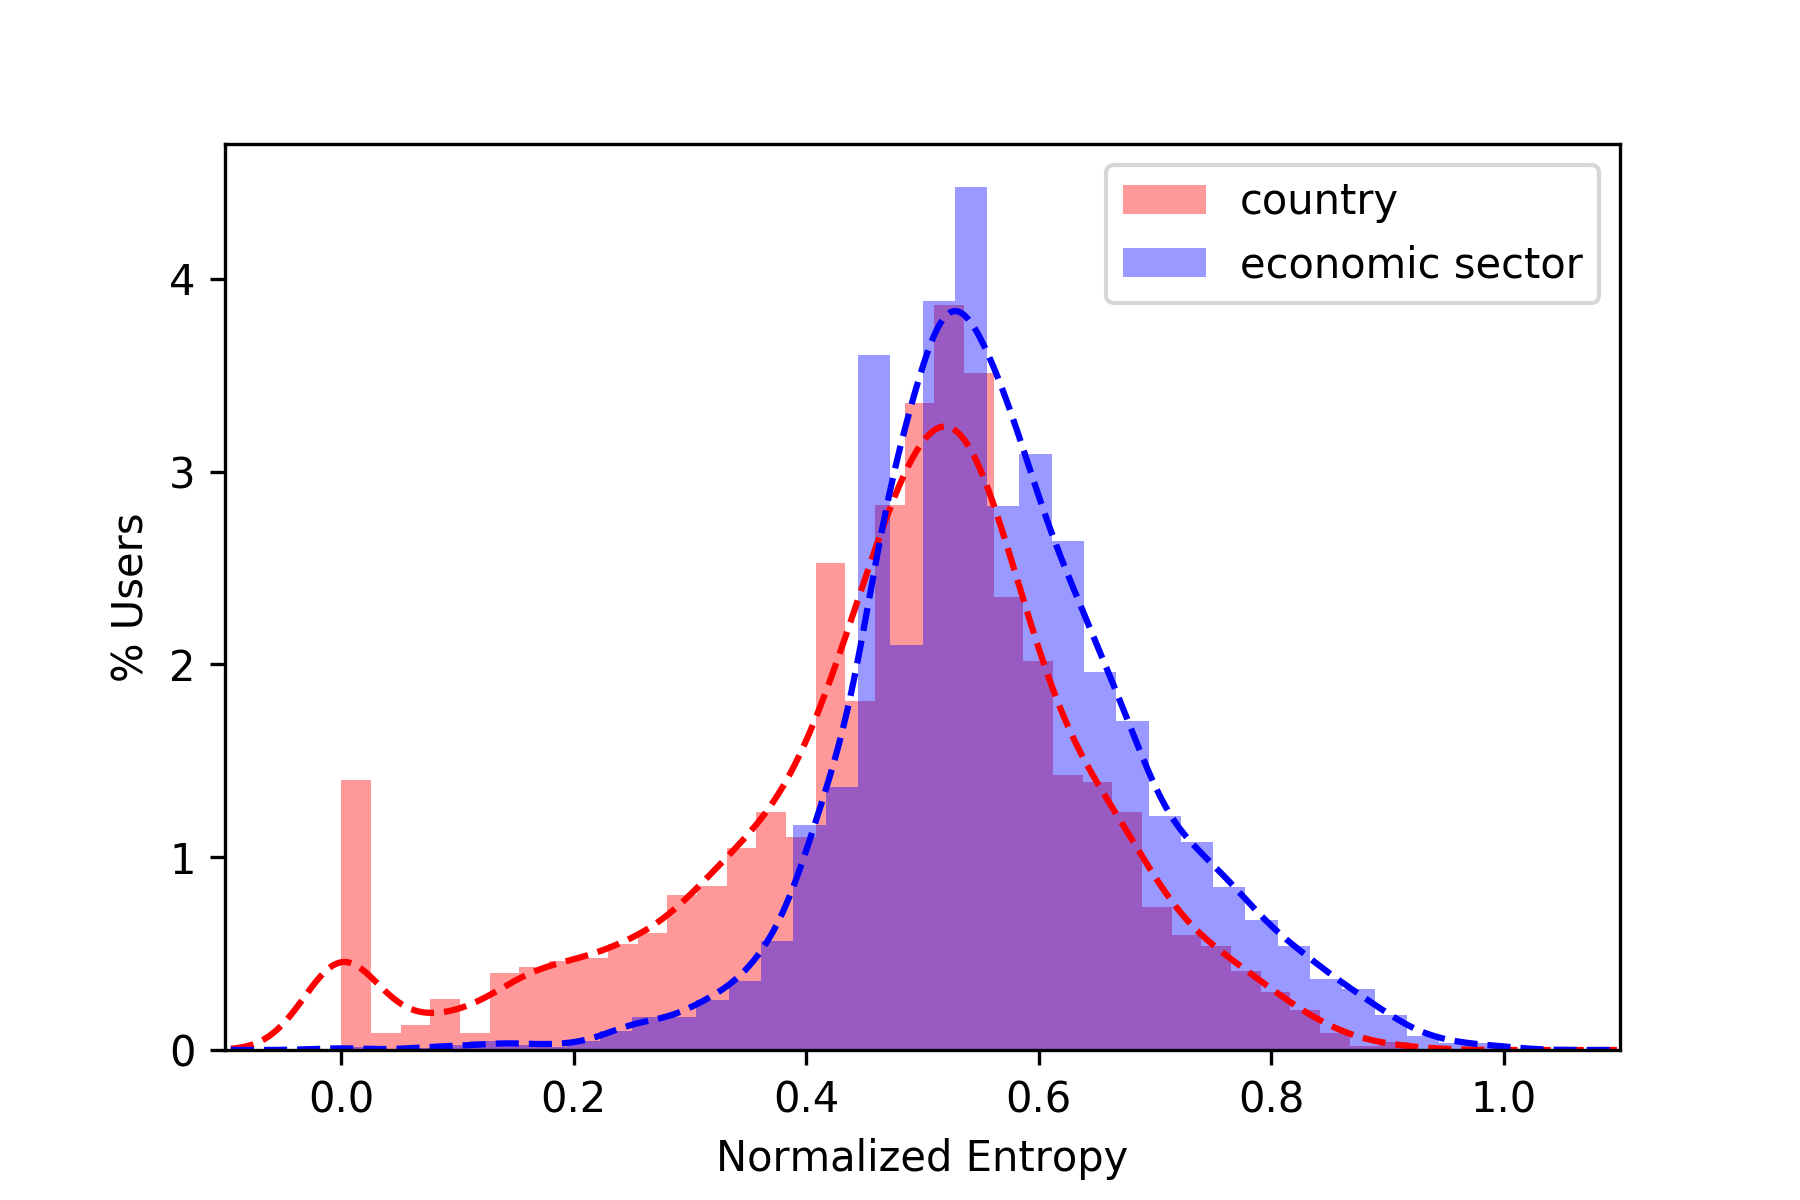
\includegraphics[width=\linewidth]{imgs/ofair/kiva_user_entropy_distribitions_lineDist.png}
    % \caption{User tolerance value ($\tau$) for feature category. Kiva dataset.}
    \caption{User tolerance value ($\tau$) for Economic Sector and Loan Country features in Kiva dataset.}
    \label{fig:tau_vector_Kiva}
\end{figure}
% \vspace{3cm}

\begin{figure}[tbh]
    \centering
    % \includegraphics[width=\linewidth]{plots/entropy_difference_ml_pro.png}
    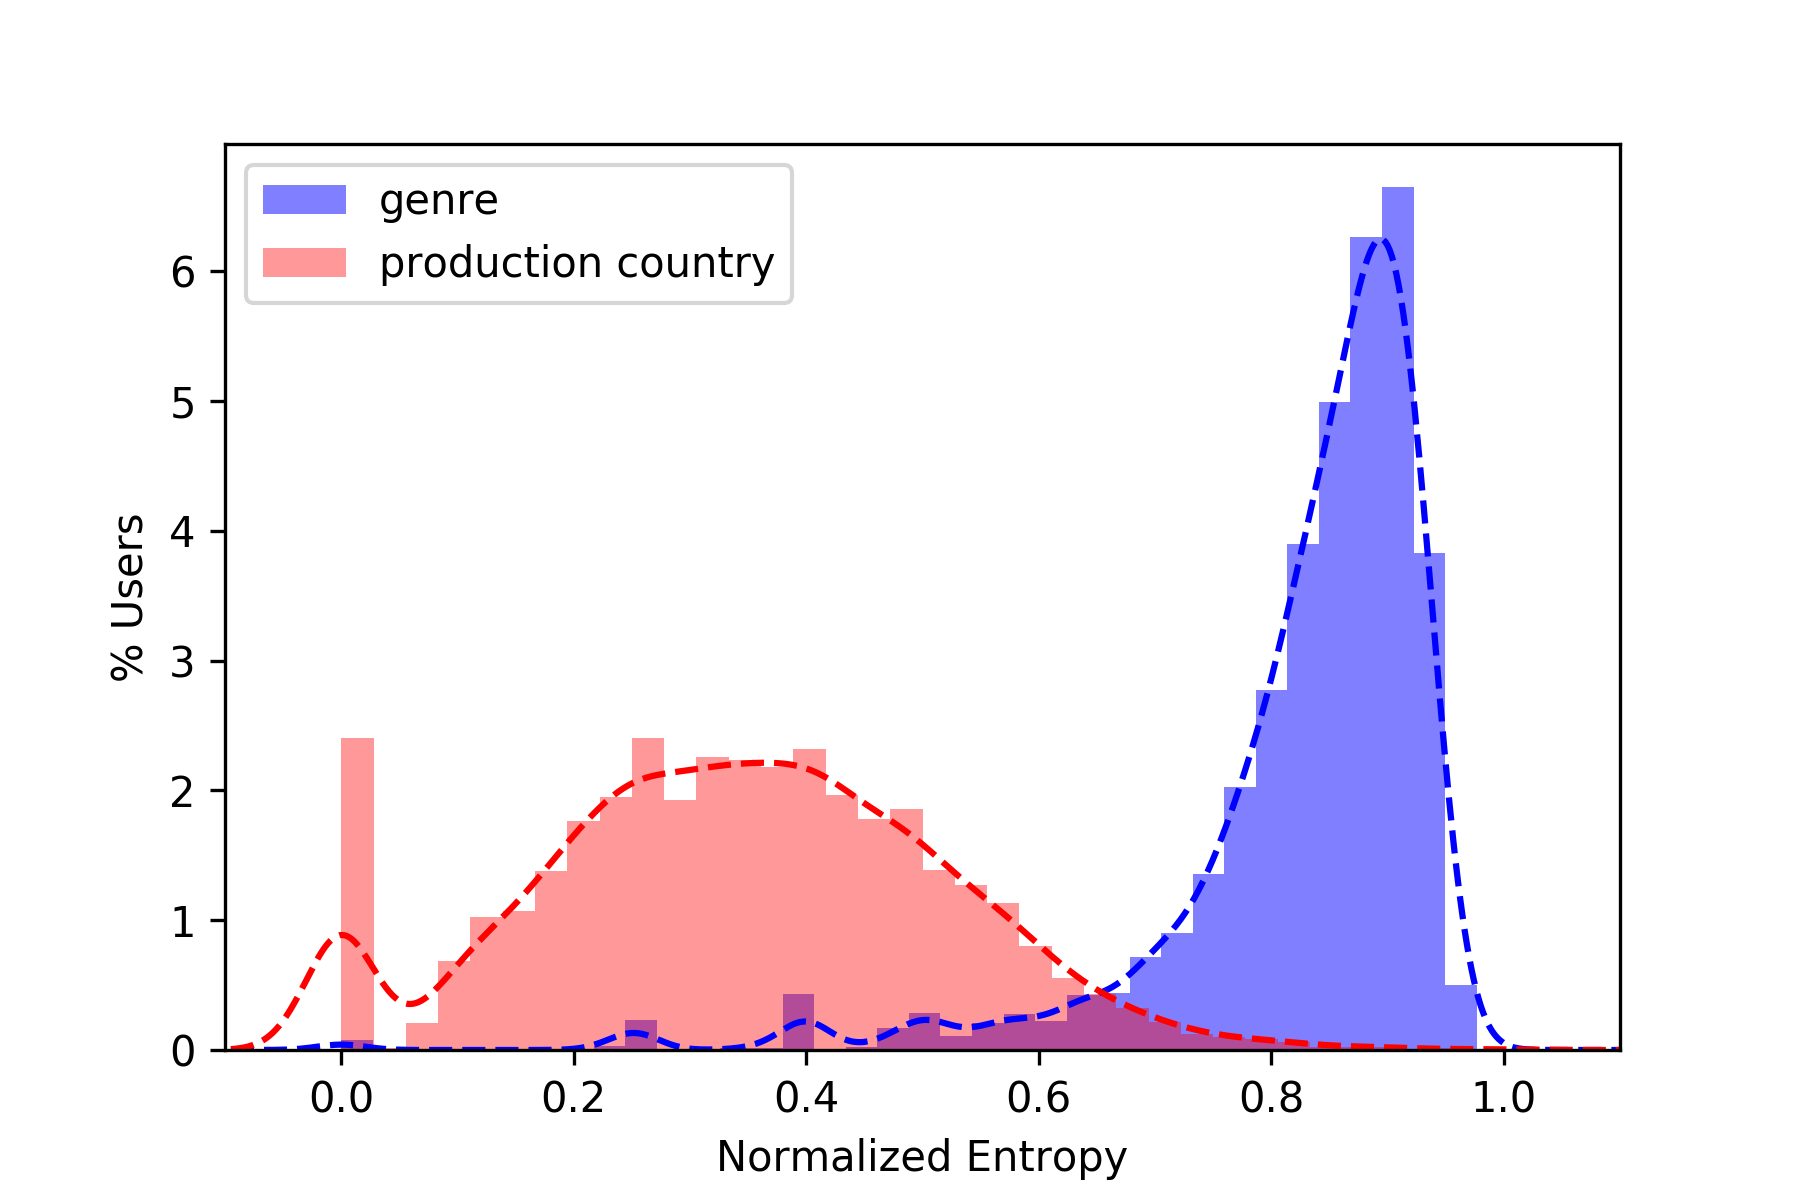
\includegraphics[width=\linewidth]{imgs/ofair/ml_user_entropy_distribitions_lineDist.png}
    % \caption{User tolerance value ($\tau$) for feature category. The Movies Dataset dataset.}
    \caption{User tolerance value ($\tau$) for Genre and Production Country features in The Movies dataset.}
    \label{fig:tau_vector_ML}
\end{figure}

Figure~\ref{fig:tau_vector_ML} shows similar results for the Movies dataset. Again, we see that users in this sample have wide individual variance in the computed $\tau$ values for different dimensions of movies. For example, the variation in the entropy for the genre dimension (shown in blue) indicates that most of the users are watching movies from various genres while there are some users who usually prefer to watch the same few genres. The variation in the production countries (shown in red) is flatter and farther to the left, indicating users' narrower choice of movies in this dimension. Possibly, these viewers mostly watch movies that are produced in their countries or in their language.

We note that different features have different baseline entropy values in each dataset. In our future work, we plan to explore a refinement of the personalized tolerance measure using conditional entropy to calculate how much each user profile adds or detracts from the entropy in a particular feature.
% For example, the gender skew in the Kiva data means that the gender feature has much lower entropy values overall than the one for economic sector. In our future work, we plan to explore a refinement of the personalized tolerance measure using conditional entropy to calculate how much each user profile adds or detracts from the entropy in a particular category.

\paragraph{\textbf{Comparing re-ranking algorithms}}
We use non-negative matrix factorization as our baseline recommendation component. The algorithm was tuned on each dataset separately to achieve the best nDCG. The algorithm was trained on 80\% of the data and tested on the remaining 20\%. The nDCG of NMF was around 0.11 on the ML dataset and 0.076 on the Kiva dataset.
For each algorithm, we retrieve $k=200$ top items for each user and re-rank the list retaining the top $k'=10$ items.  

In our experiments, we compared our OFAiR algorithm with FAR and PFAR, as our baseline methods. We also used MMR by itself, as a diversity-enhancing re-ranker, a variant of OFAiR that includes only user tolerance weights for each feature, and a variant that includes only the fairness weights for the protected feature dimensions without the tolerance weights. In this way, we can study separately the contribution of each of these aspects of the algorithm.
% , without weighting the protected and unprotected feature values

\begin{table}[]
\begin{tabular}{lllll}
 Algorithm &  1\% & 2\% & 3\% \\
 \hline
 FAR & 12.06\% & 12.09\% & 12.12\% \\
 PFAR & 12.07\% & 12.08\% & 12.09\% \\
 MMR &  12.22\% & 12.67\% & 13.08\% \\
 MMR w/ tolerance & 12.83\% & 13.29\% & 12.66\%   \\
 MMR w/ fairness & 14.0\% & 15.14\% & 17.03\%  \\
 OFAiR & 16.76\% & 20.14\% & 22.81\% \\
 \hline
\end{tabular}
\caption{Fairness vs \% Accuracy Loss. Kiva dataset. 
Larger values mean improved fairness at the given accuracy level.}
\label{tbl:kiva_fairness_accuracy_relationship}
\end{table}

Table \ref{tbl:kiva_fairness_accuracy_relationship} summarizes the results across the different algorithms. We indicate the tradeoff between fairness and accuracy by reporting the (interpolated) protected item exposure at different levels of nDCG loss: 1\%, 2\% and 3\%. We arrive at the exposure values in the table by assuming a locally-linear relationship of nDCG and fairness/exposure in between different $\lambda$ values, basically locating intercepts in the tradeoff graph. (See below.) The table shows that FAR and PFAR do little to improve fairness in this setting. This is not surprising as these algorithms were designed for a situation in which fairness across a number of different providers is sought, rather than the protected item balance situation here. In Figures \ref{fig:kiva_mmr_based_methods}, and \ref{fig:ML_mmr_based_methods} below, we will omit FAR and PFAR for this reason. Of the other algorithms, we see a small advantage for OFAiR at the 1\% level of loss, increasing greatly at higher levels of loss. Both tolerance weights and fairness weights contribute to the results but their synergy in the OFAiR algorithm is apparent. It must be noted that in absolute terms, the fairness enhancement is somewhat disappointing. 16.76\% to 20.14\% increase still means that only 1.2 protected items will appear (on average) in each user's recommendation list. 

Table \ref{tbl:ML_fairness_accuracy_relationship} shows even stronger findings in favor of the OFAiR algorithm on the Movies dataset. Two trends are noticeable. One is that there is very little change in fairness for increased $\lambda$ values in the MMR and MMR with tolerance cases. This trend also exists in Kiva dataset. OFAiR is a clear improvement at all levels of nDCG loss, although in absolute terms the improvement is still small.


\begin{table}[]
\begin{tabular}{lllll}
 
 Algorithm &  1\% & 2\% & 3\% \\
 \hline
 FAR & 28.65\% & 28.64\% & 28.64\% \\
 PFAR & 28.63\% & 28.63\% & 28.63\% \\
 MMR &  28.44\% & 29.28\% & 29.92\% \\
 MMR w/ tolerance & 28.99\% & 30.83\% & 32.13\%  \\
 MMR w/ fairness & 32.51\% & 34.44\% & 35.85\%  \\
 OFAiR & 36.59\% & 39.41\% & 41.34\% \\
 
 \hline
\end{tabular}
\caption{Fairness vs \% Accuracy Loss. The Movies Dataset.}
\label{tbl:ML_fairness_accuracy_relationship}
\end{table}

Figure \ref{fig:kiva_mmr_based_methods} shows the results on the Kiva dataset for just the MMR-based algorithms: MMR, OFiAR, and the two versions incorporating different aspects of the OFAiR algorithm, tolerance weights (users) only, and fairness weights (items) only. The figure compares ranking accuracy in the form of nDCG versus the average exposure for protected items across recommendation lists. The figure gives a more complete picture of this tradeoff than the tables above, but generally tells the same story.

% The general trend shows that by incorporating re-ranking, the algorithms move the fraction of protected group items from around 5\% to greater than 15\%.
The general trend shows that by incorporating re-ranking, the algorithms move the fraction of protected group items from around 11\% to greater than 34\%. At the higher values of $\lambda$, the algorithms are quite similar, as might be expected. When we push the algorithms to focus more on fairness, differences emerge. The OFAiR and the MMR variant with only fairness weights are very similar until we get to nDCG loss around 0.1\%. At this point, the OFAiR algorithm dominates this tradeoff in terms of nDCG while keeping the fairness comparable. MMR and MMR with tolerance have curves that are essentially vertical, with very small fairness gain from diversification.
% The OFAiR and the MMR variant with only fairness weights are very similar until we get to nDCG loss around 1\%. At this point, the OFAiR algorithm dominates this tradeoff in terms of both nDCG and fairness. MMR and MMR with tolerance have curves that are essentially vertical, with very small fairness gain from diversification.

\begin{figure}[tbh]
    \centering
    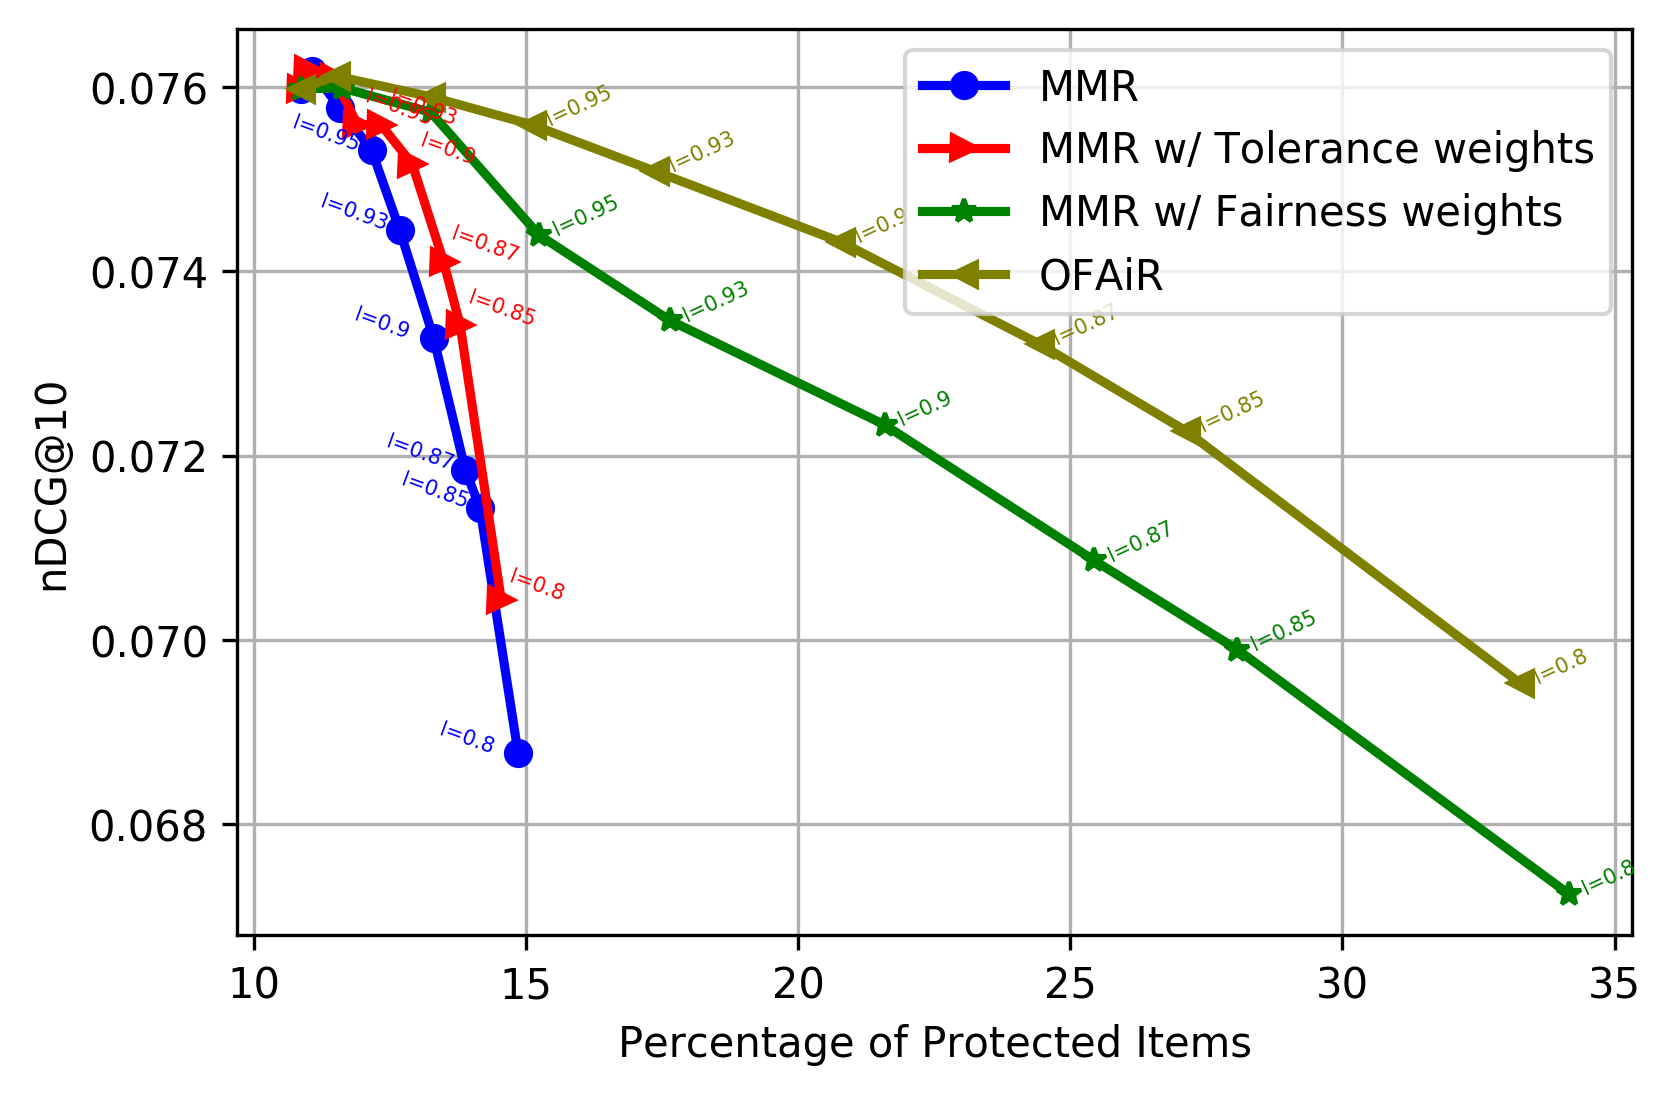
\includegraphics[width=\linewidth]{imgs/ofair/kiva_ndcg_itemCov_ActivityCountry_cut.png}
    \caption{MMR-based re-ranking methods. Kiva dataset.}
    \label{fig:kiva_mmr_based_methods}
\end{figure}

Figure~\ref{fig:ML_mmr_based_methods} shows similar results for the Movies dataset. As suggested by Table \ref{tbl:ML_fairness_accuracy_relationship}, both MMR and MMR with tolerance fare poorly as fairness is emphasized. \footnote{Although note the small but intriguing bump for the tolerance-weight-based algorithm near $\lambda = 0.95$).}
This finding highlights the difference between a user-centered view of diversification, which MMR is targeted towards, and a fairness-oriented, provider-centered view. This effect may be due to the large feature diversity present in the Movies dataset. There are many ways for movies to be diverse without falling into the protected group. 

The difference between datasets is also apparent in the relative performance of the tolerance-weighted and the feature-weighted version of the algorithm. In the Kiva dataset, fairness weights greatly enhanced fairness, competing with the OFAiR algorithm at some points in the parameter space while in the Movies dataset OFAiR surpasses all the others except in higher lambdas. The other difference is in the effect of these algorithms on the percentage of protected items achieved. As it is shown, we achieve higher fairness gains in the Movies compared to the Kiva dataset.
These differences in performance could be due to domain differences in feature distributions, such that diversification along a preferred dimension does not necessarily yield protected items. The feature weights are needed to shift the algorithm's attention to the protected parts of the feature space. As before, much larger fairness gains are possible with OFAiR.

\begin{figure}[tbh]
    \centering
    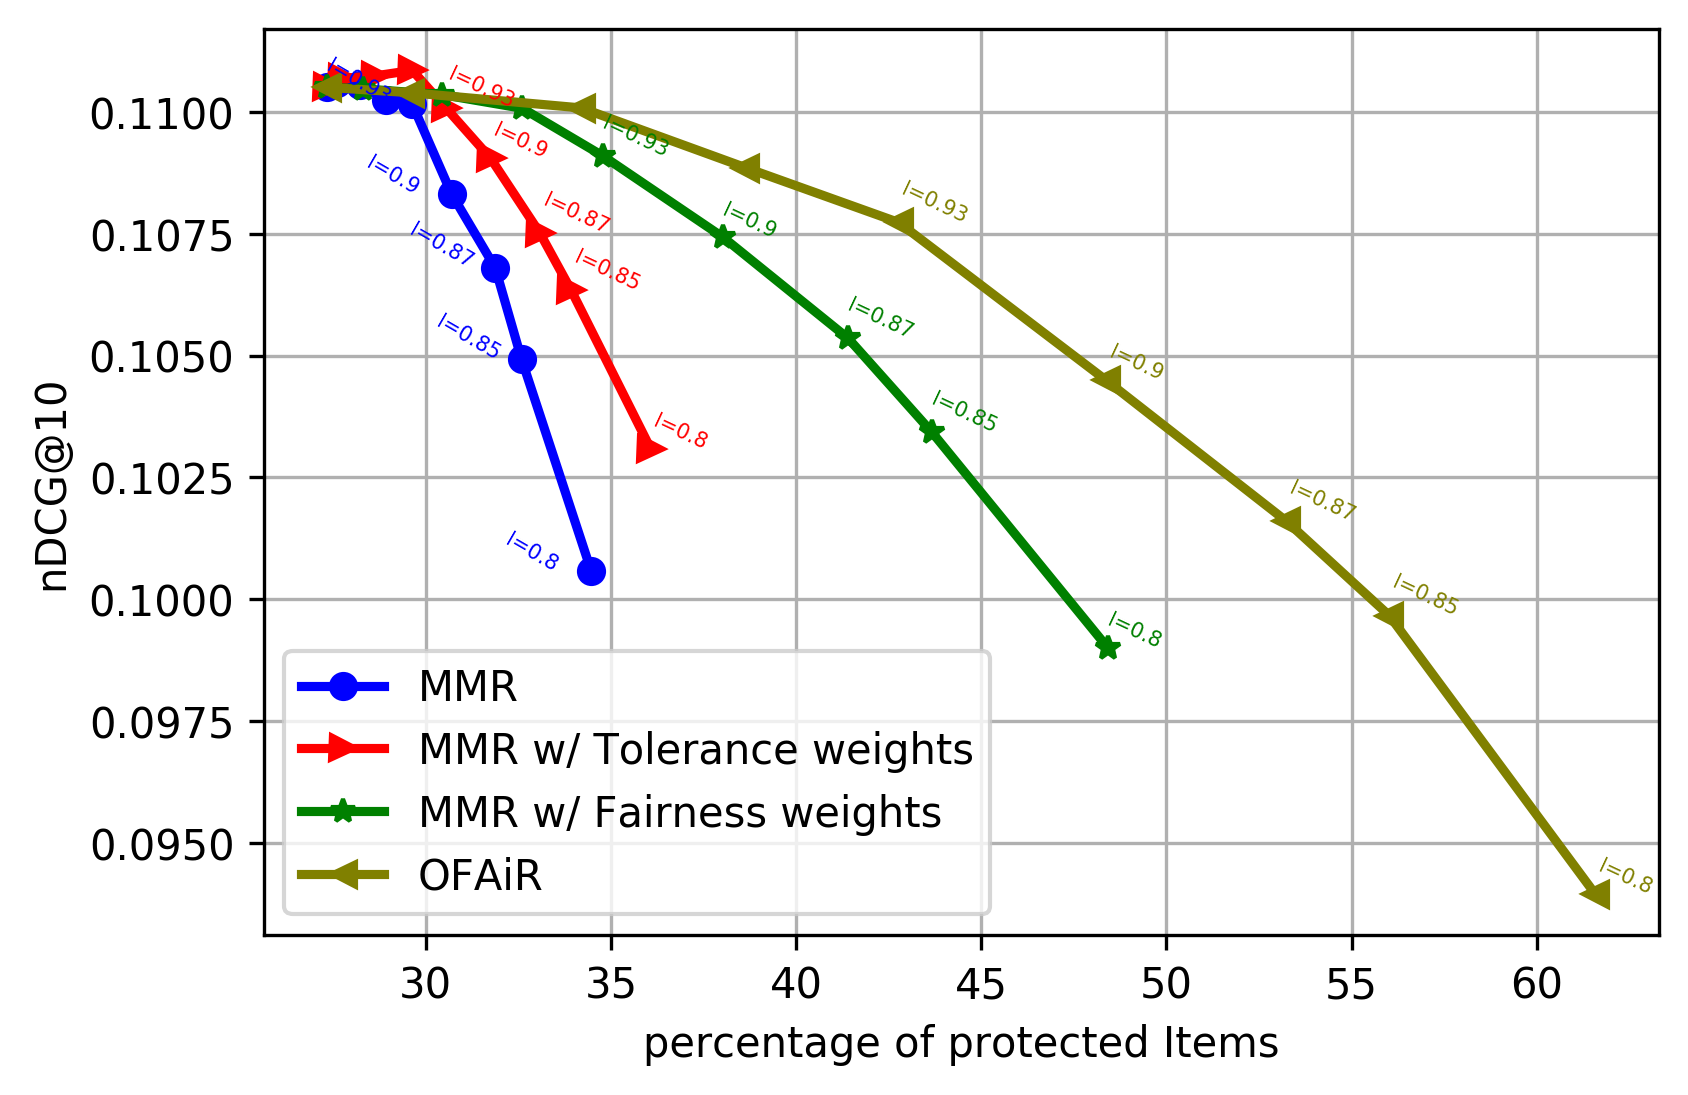
\includegraphics[width=\linewidth]{imgs/ofair/ml_ndcg_itemCov_CountryGenre_cut.png}
    \caption{MMR-based re-ranking methods. The Movies Dataset.}
    \label{fig:ML_mmr_based_methods}
\end{figure}

It is significant that OFAiR has a dominant position among the other algorithms in terms of the fairness / accuracy tradeoff when viewed across all items in the protected group.
However, a key objective of this work was to ensure distribution of fairness enhancement across multiple categories of protected groups. Figure \ref{fig:kiva_category_heatmap} and Figure \ref{fig:ML_category_heatmap} show this aspect of our experimental results.

\begin{figure}[tbh]
    \centering
    \includegraphics[width=\linewidth]{imgs/ofair/kiva_heatmap_ActivityCountry.png}
    \caption{Cross-category fairness of MMR-based algorithms. Kiva dataset.}
    \label{fig:kiva_category_heatmap}
\end{figure}

\begin{figure}[tbh]
    \centering
    \includegraphics[width=\linewidth]{imgs/ofair/ml_heatmap_CountryGenre.png}
    \caption{Cross-category fairness of MMR-based algorithms. The Movies dataset.}
    \label{fig:ML_category_heatmap}
\end{figure}

In Figure \ref{fig:kiva_category_heatmap} and \ref{fig:ML_category_heatmap}, we can see the performance of all the algorithms in terms of improvement in the exposure of the protected items in each protected dimension in a more fined-grained manner. Recall that in the Kiva dataset, country and economic sector (shown as activity) were the sensitive features with 23 countries and 5 sectors labeled as protected. It is also worth mentioning that in both of these features, users had a high general entropy as well. The lighter colors show an improvement in fairness. As it is shown, the colors are darker in NMF and MMR. The right side of the heat-map contains lighter colors indicating more inclusion of protected items in recommendation lists. Lightest colors might belong to MMR with fairness weights, and after we add the tolerance weights to the algorithm it becomes slightly darker. This is due to the fairness/accuracy tradeoff noted above. For some feature values in \ref{fig:kiva_category_heatmap}, fairness is not improved by any algorithm. This is because the reranker can only improve the fairness of the results if these dimensions are present in the recommendation list of users and in these cases they rarely are. A similar trend is found in the Movies dataset, with the OFAiR algorithm, showing the best exposure across all of the protected dimensions. 


\subsubsection{\textbf{Related work}}
\hfill

In examining prior work on re-ranking, it is important to note the distinction introduced in Section~\ref{sec:backgroundd} above between user-oriented results diversification and fairness/provider-oriented re-ranking, which is the objective of our work. A user-oriented method will measure success by the diversity of individual lists, whereas a provider fairness approach will be measuring outcomes for providers, especially protected ones.

One of the first efforts to increase diversity in recommendations was \cite{Ziegler:2005:IRL:1060745.1060754}, which used a taxonomic content-based similarity metric to re-rank recommendation lists. This method did not attempt to personalize its ranking goal relative to different users. The taxonomic item similarity measure used in this work may be appropriate to adapt to OFAiR, which currently uses a one-dimensional representation of item features. A steady stream of user-oriented diversification research followed, as summarized in \cite{kunaver2017diversity}.

More closely related to the present work are the FAR/PFAR algorithms in \cite{liu2018personalizing,liu2019personalized}, which have served as an inspiration here. PFAR incorporates the individualized entropy-based user tolerance weight, thus enabling it to increase accuracy for the users with more fixed tastes. As noted above, however, PFAR is based on the aspect-oriented xQuAD algorithm, which has a binary inclusion objective. Once a provider is represented in the recommendation list, it is no longer boosted in re-ranking. This makes sense for the FAR/PFAR use case, which concentrates on fairness across multiple providers. This is less appropriate for a protected/unprotected binary distinction because the objective is satisfied with only a single protected item included and there is therefore no way to approach parity of representation. This can be seen in the very small improvements in exposure found with these algorithms. 

Another approach to fair ranking is the FA*IR algorithm proposed in \cite{zehlike2017fa}. This algorithm creates two queues: one of protected and one of unprotected items, and then integrates them to satisfy (in expectation) a probabilistic ranked fairness test. This algorithm does make the protected/unprotected assumption that we are using in this work. However, it applies only to a single such distinction. It might be interesting to extend the FA*IR model to multiple dimensions of fairness.

Fairness for multiple groups has been addressed in classification settings under the idea of \textit{rich sub-group fairness}~\cite{kearns2017preventing,kearns2019empirical}. In this work, the emphasis is on extending fairness guarantees to all possible combinations of protected groups in a dataset. The SUBGROUP algorithm alternately optimizes for a particular group's fairness and then seeks the group for whom fairness is most violated. In recommendation, we are not seeking a single decision rule, so we have a different solution in OFAiR: to distribute the optimization ``cost'' across different users in a personalized way.

\subsubsection{\textbf{Conclusion and Future Work}}\label{sect:conclusionn}
\hfill

The results of our experiments show that OFAiR works as intended. Its proportion-based MMR model provides a much better tradeoff between ranking accuracy and fairness for the protected-unprotected case than the FAR/PFAR models explored in prior work. In the datasets under study, we show that users' tolerance for diversity varies across features, which justifies our approach of differentiating users based on the opportunities they represent for enhancing provider-side fairness. 

We show that the combination of personalized, feature-specific, weights together with weights identifying protected feature values is effective with the feature-specific tolerance helping maintain accuracy and the feature weight promoting protected group items. As we showed, our method can be applied across multiple protected groups at the same time and can ensure fairness with respect to system's designed fairness goal for each feature.

One of the challenges in this work is the lack of proper datasets that have user features and these datasets are specifically lacking in domains where fairness matters. Due to this issue, we chose the Movies dataset to show the capabilities of our method.

As our future work in this section, we intend to run a more thorough experimentation with weights of the weighted cosine similarity and capture the influence of these weights on the final results. We also intend to use different recommendation algorithms as the base recommendation.

A more general method to use is the metric learning approach, that assumes different dimensions and assigns weights to these dimensions accordingly. This is useful as it automatically assigns weights to dimensions not manually.
The other approach to explore is to use voting methods in the fair resource allocation literature in the computational social choice field. Specifically, the cake cutting problem, where we want to allocate cake slices fairly where we assume users have different preferences for different layers of the cake which is similar to our research problem here, where users have different preferences over different dimensions.

The results of this experimentation is intended to be submitted to the ACM FAcct 2021 conference.

In our next work, we intend to explore further the idea of ``opportunity'' in subgroup-fairness-aware recommendation. In particular, when recommendations are delivered over time, prior outcomes relative to different protected groups may dictate what opportunities should be most salient at any given moment. We intend to publish this work later this year in The ACM Series on Recommender Systems.

\section{Fairness in Dynamic Recommender Systems}
% SCRUF framework
% In addition to the core property of accurate personalization -- delivering results that match user interests and preferences -- recommender systems may need to satisfy other, non-accuracy, constraints in certain applications. One property of interest that has received significant attention recently is \emph{fairness}: a constraint that a recommender system should try to distribute its benefits fairly across different stakeholder groups \cite{yao2017beyond,burke2018balanced,ekstrand2018exploring,liu2019personalized,kamishima2016model,beutel2019fairness}. For example, all else being equal, a job recommender system should not recommend executive jobs to male users and clerical jobs to female users.

% Key stakeholder groups in recommender systems are often identified as \textit{consumers}, individuals who receive recommendations from the systems, \textit{providers}, stakeholders for the items that are being recommended, and the \textit{system} or platform. Fairness concerns may arise from either consumers or providers~\cite{burke_multisided_2017}. In the job recommendation case above, it was fairness across groups of consumers that is of interest. 

In this section, we focus on the problem of \textit{provider fairness}: namely, how to ensure that a recommender system, over time, is recommending items from protected groups in a fair manner relative to others. We are interested in a multi-aspect version of this problem, where items may be associated with multiple, intersecting, protected groups.

\subsection{“And the Winner Is...”: Dynamic Lotteries for Multi-group Fairness-AwareRecommendation}

Our motivating example is drawn from the peer-to-peer micro-lending platform, Kiva.org. The users of Kiva are lenders, who support entrepreneurs usually from developing countries by lending small amounts. The organization has the goal of providing equitable access to capital across different regions, economic sectors and borrower demographics. This organizational mission needs to be embedded in any system deployed to recommend loans to funders. Without some control over the characteristics of the recommendations delivered, it is easy to imagine that a positive feedback loop \cite{sun2019debiasing} could develop in which some types of loans are increasingly disadvantaged by the algorithm.

In general, we may anticipate that a fairness-aware recommender system will need to respond to multiple \textit{fairness concerns} simultaneously. In this work, we adopt a social choice perspective \cite{BCELP16a} on balancing different fairness concerns, which gives us a rich set of normative properties and algorithms. Social choice is fundamentally concerned with combining preferences from multiple parties into a single outcome in which all parties participate, voting being a paradigmatic example of such a choice~\cite{Zwicker:Voting}. We can think of each fairness concern as a kind of actor, with preferences over which recommendations should be delivered. Combining the preferences of multiple such concerns fits squarely into the social choice realm.

We believe that social choice is a more flexible and realistic framework for representing fairness-aware issues in machine learning than the optimization frameworks typically employed. Social choice is inherently multi-agent, and therefore, the idea of the integration of multiple fairness concerns naturally emerges, rather than being a complex add-on. Importantly for recommendation problems, social choice naturally allows for heterogeneity and hence personalization across decision instances since a user is just another agent with preferences over the outcome. Finally, fairness is inherently a social and political construct, and a social choice formalization allows the preferences of different actors to be foregrounded, rather than relegated to the black box of machine learning optimization. The study of fairness has a long history in the social choice literature \cite{Young:Equity,Zwicker:Voting}.

\paragraph{Contribution}

In this project we propose a novel framework for recommender systems we call \textit{Social Choice for Re-ranking Under Fairness} (SCRUF). SCRUF uses multiple fairness metrics to evaluate the history of recommendation delivery and determine whether and how to adjust its performance. It uses feature-specific re-rankers to improve fairness, selecting one re-ranker (possibly non-deterministically) at each time point. We use a set of social choice inspired algorithms to allocate re-rankers to users based on the user preferences. This framework abstracts the particular fairness metrics away from the recommendation algorithm design, an approach that becomes unwieldy when attempting to incorporate multiple fairness concerns. It also supports a dynamic balance between the interplay between personalization and fairness and is therefore sensitive to context and individual differences. We demonstrate the efficacy of our design on two recommendation domains.
%Given a set of fairness metrics, possibly a different one for each sensitive attribute in the set of items, and recommendation algorithm, SCRUF uses a re-ranking approach to adjust its performance based on the historical view of recommendations that have been delivered over a time horizon, dynamically re-balancing between fairness concerns.  

\subsubsection{\textbf{Fairness-aware Recommendation}}
\hfill
% A substantial body of research on fairness in machine learning, especially in classification settings, has emerged in the past ten years, including formalizing definitions of fairness~\cite{chouldechova2017fair,dwork2012fairness,hardt2016equality,narayanan2018translation} and offering algorithmic techniques to mitigate unfairness~\cite{kamiran2010discrimination,pedreshi2008discrimination,zemel2013learning,zhang2017anti}. Fairness in recommender systems emerged as a research topic more recently, first in the work of Kamishima et al. in 2012~\cite{kamishima2012enhancement}, and the topic has since drawn increased attention~\cite{burke_multisided_2017,yao2017beyond,kamishima2018recommendation,burke2018balanced,fatrec-workshop-2017,fatrec-workshop-2018,pmlr-v81-ekstrand18b,mehrotra2018towards}. Recommender systems, while a subclass of machine learning systems, are different enough that the results from classification cannot be readily applied. Chief among these challenges is the issue of personalization. A recommender system is supposed to deliver suggestions tailored to each user's preferences, providing every user with a different experience. As such, it differs from a classifier that establishes a classification function with a single decision boundary for all cases.

Both in the machine learning and the recommender systems formulation of fairness, there has been little recognition of the intersection of multiple fairness definitions and dimensions, although recent work has noted the benefits of combining multiple fairness definitions~\cite{beutel2019fairness}. Most existing research considers only a single protected class, and even in cases where multiple groups are considered as in~\cite{buolamwini2018gender,hebert2018multicalibration,kearns2017preventing,zhu2018fairness}, fairness is conceived the same way for all groups. In recognition of the complexity of the fairness concept, we seek to accommodate different definitions of fairness put forward by different stakeholders, all of which must be integrated in a single framework. This nuanced understanding of the value of fairness is essential for capturing the richness of this social construct in real-world settings such as those studied by scholars of organizational justice, anti-discrimination law, and social justice.

As discussed in before, two standard approaches have emerged to integrating fairness concerns into recommender systems. The \textit{integrated} approach builds a fairness constraint into the recommendation model itself, for example as a regularization constraint, balancing between accuracy and fairness in the optimization process for the recommendation model \cite{kamishima2012fairness,yao2017beyond}. The \textit{re-ranking} approach applies fairness to the output of a recommendation algorithm, reordering the results. Re-ranking approaches offer a number of advantages. First, the trade-off between accuracy and fairness can be tuned without re-learning the recommendation model. Second, researchers have found that re-ranking can achieve better trade-offs versus accuracy with this type of model~\cite{pmlr-v81-ekstrand18b,abdollahpouri2019managing,liu2019personalized}. Due to these advantages we choose to use the latter method.

There has been some recent work in recommendation fairness that incorporates multiple fairness dimensions, most notably the OFAiR method discussed in \cite{sonboli-umap-2020}. This work integrates user tolerance towards different types of variation in item features with a representation of protected groups that spans multiple dimensions. The authors were able to show a beneficial trade-off between fairness and accuracy and improved results across different categories of protected groups. One drawback of the method of \cite{sonboli-umap-2020} is that it relies on weights associated with item features to boost the inclusion of protected group items into recommendation lists. Balancing across different groups requires careful setting of these weights and sometimes unexpected interactions arise.

In addition, this and similar methods are list-wise approaches, which aim to increase protected group representation in individual lists. However, as noted above, the real objective of fairness-aware recommendation is to enhance fairness as measured historically, across the behavior of the system as it provides recommendations to many users over time. The personalization element of recommendation means that this objective cannot be targeted directly: any given user may or may not constitute a good opportunity to enhance fairness relative to a particular protected group. In \cite{sonboli-umap-2020}, this aspect of the problem was addressed by incorporating user-specific weighting, which can be interpreted as a preference in a social choice setting. 

Analyzing user characteristics enables the system to determine which users constitute good opportunities to pursue different fairness goals. However, there is another side of the problem. At any point in time, the system's historical performance may have been more favorable to one protected group than another. If we only look at the users, we ignore the signal from past performance about where fairness needs are most critical.

\subsubsection{\textbf{Computational Social Choice for Fair Recommendations}}
\hfill

Fairness has been extensively studied in the economic field of social choice including work focusing on the division of continuous resources such as land or water \cite{Moulin:FairDivision}, on more discrete, indivisible settings such as goods and services \cite{Thomson:FairRules,Thomson:IntroFairAllocation} and more fundamentally in the areas of political economy having to do with justice and fair distribution of resources to individuals \cite{Young:Equity,Rawls:Justice,Rescher:Justice}. In its classical formulation, \emph{social choice} concerns itself with the study of how groups, where each member is endowed with their own preferences, make decisions that must be then shared by that group \cite{Sen:CollectiveChoice}. To these considerations the field of computational social choice adds computational tools including algorithms, complexity, and big data \cite{BCELP16a,DBLP:conf/ijcai/Mattei20}.


From the literature on social choice we will focus on the \emph{allocation} setting (which is a generalization of the classical matching setting) \cite{BCELP16a}. In allocation, the items within $A$ are to be distributed or \emph{allocated} to the set of agents in $N$.  Hence, the social part of social choice reinforces the idea that a set of preferences need to be considered and combined since the outcome of a social choice process will affect all the agents.  There have been many practical applications of matching and allocations from kidney allocation \cite{Roth:Kidney} to conference paper reviewing \cite{LiMaNoWa18}.  There are extensive studies of algorithms for a variety of settings \cite{Manlove:MatchingPrefs} and the study of fair allocations in multi-agent systems is a popular topic in the broad area of artificial intelligence \cite{Aziz:FairAllocation}. Equity and other concerns, formalized as economic axioms have a long history in social choice both in allocation \cite{Young:Equity} and voting \cite{Zwicker:Voting}. It is this long history of study of the axioms, or properties, of the algorithms and aspects including \emph{fairness} we hope to leverage.

Rather than thinking of integrating the concerns of protected groups into re-ranking decisions indirectly, in the form of weights for particular feature values as in \cite{sonboli-umap-2020}, our approach \textit{Social Choice for Re-ranking Under Fairness} (SCRUF) conceives of both users and protected groups as actors with preferences over the items that may be recommended. The goal is to achieve an integration of these preferences over the whole recommendation history. We explore a class of solutions to this problem that assumes multiple fairness criteria can be persued at the same time by deciding which objectives to address and which users to address them with.  This choice is made non-deterministically and also take into account both the current state of the recommendation history, which we can think of as defining immediate needs, and the user's propensity towards different item categories, which define current opportunities, in the context of providing personalized recommendation results. 

A social choice perspective on recommendation has emerged in recent research as a possible source of methods to integrate the viewpoints of multiple agents  or priorities \cite{burke2020algorithmic}. \citet{chakraborty2019equality} build a recommendation system for finding fair group recommendations through viewing them as elections between various signals of popularity, leading to a shared group recommendation.  This does not take the important aspect of \emph{personalization} into account that we address in SCRUF.  \citet{suhr2019two} explore driver assignment in two sided matching markets with an emphasis on producer and rider fairness. \citet{patro2020fairrec} propose a recommender system for two-sided matching markets with the goal of fair exposure amongst producers.  This differs from our work in that the fairness metrics are fixed and embedded into the matching algorithms themselves.  Finally, \citet{lee2019webuildai} propose a system that uses social choice to embed normative properties for algorithmic governance into the algorithms themselves, as demonstrated on a food bank matching scenario. However, none of this research considers multiple fairness concerns on the provider side of a recommendation system as required in the Kiva case or the dynamic response to historical fairness outcomes as embodied in SCRUF.


\subsection{\textbf{Formal System Specification}}
To leverage the power of recommender systems for personalized fairness we will define a set of choice functions to promote fairness. We first detail the formal notation for our recommender system and how to view it as a social choice problem. We then describe our overall system in terms of choice functions and how these can be used to promote fairness.

\subsubsection{\textbf{Recommendation Systems with Protected Values}}
\hfill

In a recommendation system setting we have a set of users $\users = \{u_1, \ldots u_n\}$ and a set of items $\items = \{v_1, \ldots, v_m\}$. For each item $v_i \in \items$ we have a $k$-dimensional feature vector $\vec{v_i} = \langle f_{i1}, \ldots f_{ik} \rangle$ over a set of categorical features $\features = \{F_1, \ldots, F_k\}$, where each feature $F_i$ has finite domain $\domain_i$. We assume that all elements in $\items$ share the same set of features. 
%
Consider a running example of a funding site that shows micro-loans in emerging markets to potential funders. In this example we have $m=3$ items in the database which share $|\features|=4$ features: $\{$Region, Gender, Sector, Amount$\}$, where each has its own domain.  For example, $\domain_1 = \{$Africa, Middle-East, North America$\}$.  This setting is illustrated in Table \ref{table:user_profile}.
    
\begin{table}
    \begin{tabular}{|c|c|c|c|c|}
    \hline
            & $F_{1}$ : Region & $F_{2}$ : Gender & $F_{3}$ : Sector & $F_{4}$ : Amount \\
    \hline
        $v_1$ & Africa & Male & Agriculture & \$0-\$500\\
    \hline
        $v_2$ & Africa & Female & Health & \$500-\$1,000\\
    \hline
        $v_3$ & Middle-East & Female & Clothing & \$0-\$500 \\
    \hline
    \end{tabular}
    \caption{Set of Potential Loans.}
    \label{table:user_profile}
\end{table}

Though our items are comprised of a set of features, we start with the view that not all features should be treated the same. We assume that there is a subset of the features $\sensitive \subseteq \features$ that are denoted as \textit{sensitive} and there is a subset of values for each such feature, i.e., $\pro_i \subseteq \domain_i$ that constitute the \emph{protected values} of the sensitive feature. That is, given all items in the recommendation system, we have a subset of sensitive features, each of which may contain protected values. Turning back to our running example, we may wish to target $\features_1=\{Region\}$ as a sensitive feature and the values $\pro_1=\{$Africa, Middle-East$\}$ as the protected values. We could designate sensitive features and protected values based on operational goals such as regions or genders that are funded less frequently.

For our recommender system we have a personalized ranking function $R(u_i, \items) \rightarrow \sigma_i(\items)$, which given user $u_i$ and set of items $\items$ produces a permutation, i.e., a ranking, over the set of items for that user, i.e. a recommendation. As a practical matter, the recommendation results will always contain a subset of the total set of items, typically the head (prefix) of the permutation $\sigma_i$ up to some cutoff number of items.

\subsubsection{\textbf{Re-Ranking Functions}}
\hfill

In order to promote fairness, we assume that we are also given a set of re-ranking functions $\rerankers = \{\kappa_1, \ldots, \kappa_{|\sensitive|}\}$, which are a set of functions, one for each sensitive feature. For feature $j$, the re-ranking function $\kappa_j(\sigma) \rightarrow \sigma^{\prime}$ will take a permutation $\sigma$ and produce a new permutation $\sigma'$ of the set of items that is more ``fair'' towards the particular protected feature values associated with $\sensitive_j$. In real applications, the final recommendation slate is a short list of the most preferred items from this final, re-ranked permutation. 

For our system we assume a common form of all re-ranking functions, where the permutation is achieved by sorting items based on a score, and the score is a linear combination of the score from the recommender system (the determiner of the original $\sigma$ ranking) and a score based on the presence of the protected feature, such that protected group items are moved up in the ranking list~\cite{adomavicius2009improving}. The scoring function $\rho$ for user $u$, an item $v$, and a sensitive feature $j$ is defined as follows:

\begin{equation}
    \rho(u, v, j) \buildrel\triangle\over= \lambda_j  (R(u,v) + (1 - \lambda_j) \mathds{1}_{\{v \in \sensitive_j\}}
\end{equation}

%\begin{equation}
%    \Delta(u_i,\ell',\ell)\buildrel\triangle\over= \arg\max_{v \in \ell' \setminus \ell} [\lambda  %(R(u,v) + (1 - \lambda) \mathds{1}_{\{v \in \sensitive_j\}}]
%\label{eq:reranker}
%\end{equation}

\noindent The indicator function $\mathds{1}_{\{v \in \sensitive_j\}}$ has the value 1 if the item $v$ has a protected value of sensitive feature $\sensitive_j$, and 0 otherwise. $\lambda_j$ is a feature-specific parameter that controls the trade-off between accuracy (as represented by the original $\sigma$ ranking) and fairness (as represented by the boost given to protected items). All of the items in the list $\sigma$ are re-scored using $\rho$, sorted in decreasing order, and truncated to produce the final $\sigma^{\prime}$ recommendation list.

\subsubsection{\textbf{Metrics for Fair Recommendation}}
\hfill

There are a wide variety of metrics that have been proposed for measuring the fairness of a recommendation result or set of recommendation results.  In our setting we are not concerned with the fairness of a particular recommendation but rather the \emph{history of recommendations} the system has generated over within some time window.  Hence we track the prior history of recommendations lists that have been generated $\vec{L} = [\ell_1, \ldots, \ell_{t-1}]$ for the users (with a slight abuse of notation) $\vec{U} = [u_1, \ldots, u_{t-1} ]$ that have appeared to the system.  

Rather than commit to one particular metric in our system, we assume a family of functions $\metrics_j: \vec{L} \times \vec{U} \rightarrow \reals$, one for each sensitive feature $\sensitive_j$, mapping from a set of recommendation results $L$ and the set of users $U$ to whom each of those results have been delivered to a value indicating the degree of fairness in the total set of results. We assume that a higher $\metrics_j$ values indicate a fairer result. Without loss of generality, we assume that each metric has values in the range $[0,1]$.

We will assume that the re-ranking functions have a non-decreasing impact on their associated fairness metric. That is, given a recommendation result $\sigma$, $\metrics_j(\sigma, u) <=  \metrics_j(\kappa_j(\sigma), u)$.  Because of this property, we can interpret a fairness score as indicating the relative number of times we want to select the different re-ranking functions. If the metrics were all equal, then the different re-ranking functions would be equally desirable.

Note that the inclusion of $\vec{U}$ as an argument to the $M_j$ functions allows us to include a family of fairness metrics that are sensitive to the user's level of interest in items that vary on different feature dimensions. Each recommendation result is then evaluated relative to the user to whom it is delivered. For example, even if our recommendation history tells us we should be favoring loans in the textile sector, it may not be as valuable to recommend such loans to the agriculture-focused user, as opposed to a user that has proved to be more flexible in which sectors they support.

\subsubsection{\textbf{User Preferences for Fairness}}
\hfill

To incorporate the social choice aspects of the problem, user preferences over both the overall set of items as well as preferences about the \emph{re-ranking functions themselves} need to be taken into account. In a traditional social choice setting we have a finite set of agents $N = \{1, \ldots, n\}$ and a finite set of alternatives $A = \{1, \ldots, m\}$. Each agent $i \in N$ has a preference $\succsim_i$ over the alternatives. Typically these preference are expressed as a binary relation (weak or linear order) over the set of alternatives $A$.  

While the user preferences are handled by the personalized ranking function $R(u_i, \cdot)$ we will also incorporate the preference over the fairness functions themselves. To this end, replacing the preferences $\succsim_i$ above, we assume that for each user we are also given a vector of real numbers, $\vec{\tau}_{u_i} = \{\tau_1, \ldots, \tau_k\}$ of length $k$, which indicates the tolerance (preference) of $u_i$ for variation relative to feature $F_k$.  We can then view our problem as one of allocating re-ranking functions to users based both on the their preferences and on the current fairness status.
 
\cite{eskan2017-personalized-diversity} introduced the concept of personalized diversity in collaborative filtering using a user-specific measure based on information entropy. High entropy in a categorical distribution of user profile represents high interest of user in diversity. Liu et al. \cite{liu2018personalizing,liu2019personalized} integrated this concept for the first time in recommendation re-ranking using a quantity $\tau_u$, a user-specific measure of interest in diversity.

\begin{equation}
\vec{\tau}_u(F_{j})\buildrel\triangle\over=-\sum_{f \in F_j} P(f|u)\log P(f|u),
\label{eq:tau}
\end{equation}

\noindent where $P(f|u)$ is computed as the fraction of items in the user's profile that have the feature value $f$. This can be interpreted as the user's likelihood of liking items with that value. The higher the entropy value is for a user on a feature, the higher their tolerance to see diversity within that feature. We assume that we can interpret this as a \emph{preference} in the social choice sense. In our running example, a user may be particularly dedicated to a particular economic sector, agriculture for example, and may only have supported loans in this sector in the past.  Hence, they would have low tolerance for variation in this feature. Note that since these map onto $\reals$ we could both interpret these as ordinal rankings: as a preference order for user $u_i$, $\succsim_i$, over the set of $f_j$; or as cardinal valuations.

\subsubsection{\textbf{Overall Framework}}
\hfill

SCRUF is our framework for explicitly representing the design decisions that enter into trading off between accuracy and fairness across multiply-defined and intersecting protected groups in the setting described above. Figure~\ref{fig:framework} shows the general process that the framework instantiates by looking at a snapshot in time. A user $u_t$ arrives at the system and the base recommender algorithm $R(u_t,\items)$ generates a recommendation list $\ell_t$. 

\begin{figure}[tb]
    \centering
    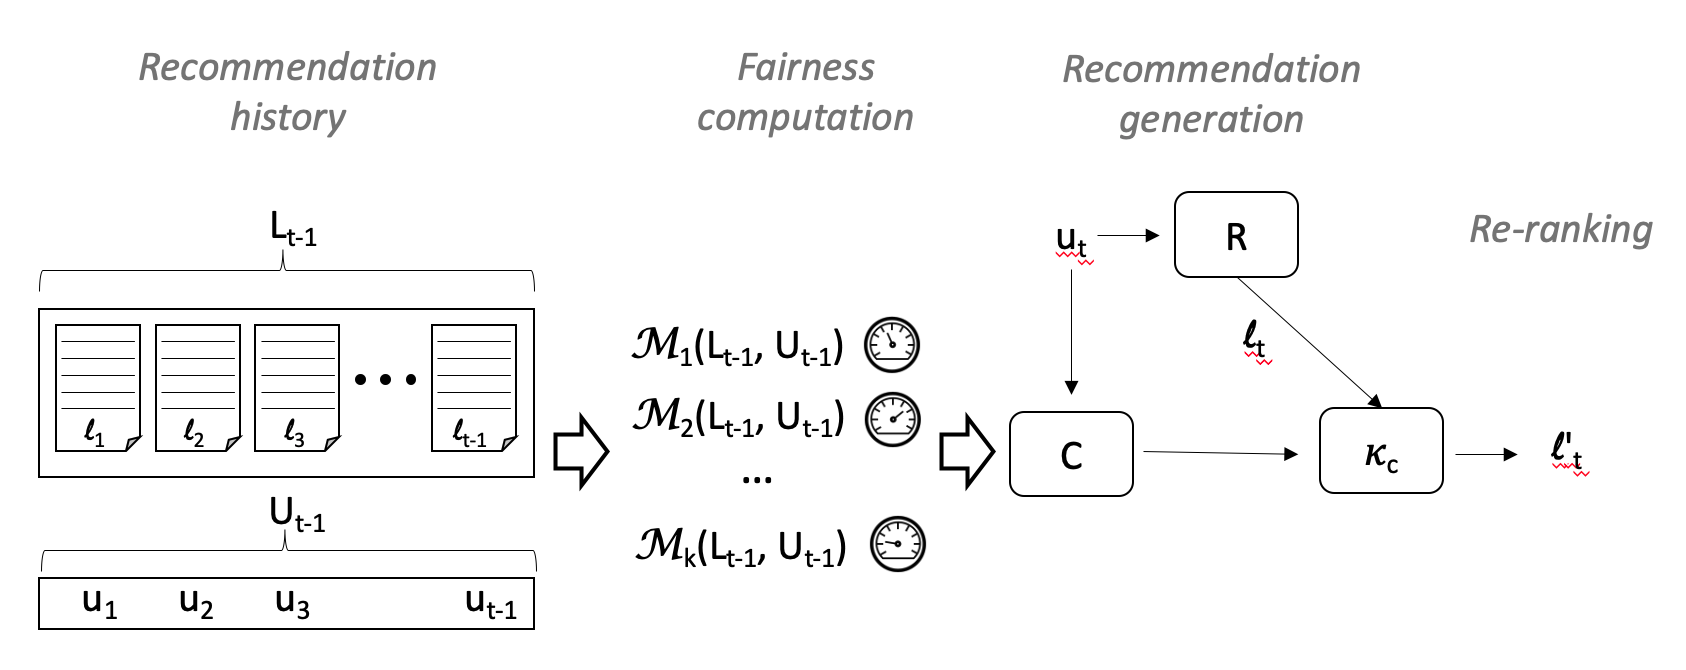
\includegraphics[width=5.5in]{imgs/dynfair/process-graphic.png}
    \caption{SCRUF framework, a snapshot at time $t$: On the left are the recommendation lists $L$ computed at prior time points. Fairness metrics $M$ compute the fairness state, which is input to the choice function $C$, selecting a re-ranker $\kappa_t$ that processes the recommendations $\ell$ from $R$ into a final re-ranked slate $\ell^{\prime}$.}
    \label{fig:framework}
\end{figure}

SCRUF is able to accommodate different metrics, one for possibly each sensitive feature, $\features_j$, $\metrics_j: \vec{L} \times \vec{U} \rightarrow \reals$.  Since we have access to the history of all recommendations, we can derive particular fairness results relative to the different sensitive dimensions indicated by the meters associated with each metric $\metrics_j$. This set of metrics are input to a choice function $C$ which picks one dimension to prioritize and selects the corresponding re-ranking function $\kappa_c$, which is applied to $\ell_t$ resulting in a final set of recommendations $\ell^{\prime}_t$ that is displayed to the user. (As a practical matter, our implementation described below groups users into batches and calculates the fairness metrics only once per batch.)

Note the arrows from the user $u_t$ point both to the recommendation algorithm $R$ where the algorithm takes into account the user's inferred preferences over items in attempting to predict the user's preferences, and also to the choice function $C$ that may take into account the user's inferred preferences from their tolerance scores $\vec{\tau}_{u_i}$ over item features in choosing a re-ranking algorithm. 


\subsubsection{\textbf{Choice}}
\hfill

As noted above, we are investigating both deterministic and non-deterministic mechanisms for selecting, at each point when a recommendation is generated, a single $\kappa_j$ function to use to re-rank those recommendation to a specific user $u_j$. The choice function $C$ uses the current state of the recommendation history, as defined by the $M_j$ metrics over the recommendation history so far and optionally the identity of the current user, to compute a feature $c \in \sensitive$  whose corresponding re-ranking function $\kappa_c$ will be applied to the recommendations for this user, i.e., $\kappa_c(R(u_j, \items))$. We prefer this simple uni-dimensional re-ranking scheme over one that attempts to incorporate multiple fairness dimensions are considered at once because it creates independence between re-ranking operations and avoids complex parameter interactions that might occur in attempting to compute a single re-ranking incorporating multiple fairness dimensions.

One issue that may arise, and we discuss in the next section, is that we need to decide when to \emph{stop} running the re-rankers for a particular feature. If the historical data at time $t$ shows that we have been fair towards a particular feature, we do not need to promote it in this iteration. In the following we will describe how we select which features to consider.

\subsection{\textbf{Choice Functions}}

What remains to be specified within the SCRUF framework is the choice function $C$. There are wide variety of ways such a function could be formulated. In this work, we explore three different variants of the lottery, where probabilities are set for each re-ranker and a single re-ranker is chosen by sampling from this distribution.

In order to pick a choice function at time $t$ we will, for operational concerns, also have a parameter $w_b$ which defines the historical (backward) \emph{window} over which we are concerned with our fairness metric.  This means that our fairness metrics $\metrics_j$ are run over over the set of users and lists between $[t - w_b - 1, t-1]$.  Recall that our fairness metrics are all in the range $[0.0, 1.0]$ with $1.0$ representing full fairness for that metric.  In a slight abuse of notation we will use $\metrics$ to represent this list of values.

Also, for operational reasons, we are given an $\epsilon$ which represents a non-zero cutoff or tolerance for each metric.  We will only consider running re-rankers when $\metrics_j - \epsilon > 0.0$. This allows us to focus on the sensitive features with greater unfairness and provides a way to guard against an over-emphasize on protected groups at the expense of accuracy.

Let the \emph{unfairness vector} be (point-wise) $\vec{UF} = 1 - (\metrics - \epsilon)$.  Intuitively, this captures how unfair we are being towards a particular feature.  The following discussion will treat this vector as a probability distribution, and so it will be normalized to unit length, $\vec{UF} = UF / \sum_i(UF_i)$.  \farzad{This does not look correct!} Note that this will implicitly assume that our target each element of $UF = 1/|UF|$, i.e., that we want unfairness to be equal across all aspects.  This is a byproduct of our metrics taking values in $[0.0,1.0]$ since if all metrics were $1.0$ then our normalization would be undefined, hence the $\epsilon$.  Normatively, this makes sense in that if we are being unfair the same amount to all sensitive features then we want an equal probability distribution over all features.

\subsubsection{\textbf{Baselines}}\label{sec:static}
\hfill

We employ two simple baseline techniques to contrast with the more dynamic options discussed below. The simplest is the \textit{Fixed Lottery}, in which each re-ranker is chosen with equal probability for each set of recommendations delivered. This method has the benefit of great simplicity and does not require any bookkeeping about the historical fairness of the system. 

If we want to use the information in the $UF$ vector, another simple alternative is a deterministic \textit{Least Misery} algorithm, in which we identify the feature in the $UF$ with the highest value (most unfair) and chose the associated re-ranker. This method directs the system's attention to the dimensions with the worst historical performance and attempts to correct that. It will be dynamic in the sense that as the performance improves in one dimension, another may be chosen. 

\subsubsection{\textbf{Dynamic Lottery}}
\hfill

We have found that it is typical for some dimensions to be more difficult to achieve fairness for than others. In particular, some types of items are rarely retrieved by the base recommendation algorithm and therefore only small improvements can be had through re-ranking. Applying the least misery algorithm in such a setting could lead the system to concentrate all of its effort on one of these intractable dimensions and miss opportunities to achieve fairness in other parts of the item space. 

To avoid this problem, we can use $UF$ as a lottery over the re-rankers and select a re-ranker with probability proportional to its weight, so that the poorest performing dimensions (most unfair) would have highest probabilities of being chosen. This is a \textit{Dynamic Lottery} as opposed to the fixed version above, because the probability associated with each re-ranker will change as a function of system performance. 

\subsubsection{\textbf{Allocation Lottery}}
\hfill

While the above method is sensitive to the dynamic properties of the system, it is not sensitive to each user's particular propensity or interest towards different dimensions. In prior work, the ability to re-rank selectively based on user characteristics was found to yield a better tradeoff between accuracy and fairness~\cite{liu2019personalized,sonboli-umap-2020}. For this reason we consider in this section \emph{randomized allocation mechanisms} that consider both users and fairness concerns.  In a such a mechanism we compute a fractional allocation that we can then sample from in order to compute an assignment.  So, for a given set of $n$ agents and $m$ objects, we compute a bi-stochastic matrix of size $n \times m$ which represents the fraction of a particular item is allocated to an agent.

We use a modification of the \emph{probabilistic serial (PS)} mechanism \cite{bogomolnaia2001new}.  In PS, also known as the simultaneous eating algorithm, each object is considered to have an infinitely divisible probability weight of one.  To find the allocation every agent, simultaneously and at the same speed, begins ``eating'' their most preferred object that has not been completely consumed already.  Once an object is consumed, the agents move to their next most preferred object until all objects have been consumed. The random allocation of an agent by PS is the amount of each object he has eaten. PS satisfies a number of important fairness and efficiency criteria \cite{Aziz:EqulibriaPS,Aziz:EgalRandom} and has been used in real allocation settings such as course selection at universities \cite{budish2013designing}.

In translating our recommendation system setting to use PS we use again the tolerance values $\tau$ of the agents as representative of their preferences. As PS only requires ordinal preferences we simply use the ordering and not the actual values (breaking ties randomly when needed). A key concept in PS is the idea of an object's capacity, how much it is available to be allocated. 
We set the capacity of each re-ranker to mirror the sampling lottery probability from above.
Specifically, each re-ranker has weight $w_f * UF_i$, thus limiting the amount of that re-ranker to allocate.
% \nasim{we didn't describe w_f either in facctrec :| } 
We then run the PS algorithm and get a fractional allocation for each user for each re-ranker.  We interpret this fractional allocation (normalized into a distribution) as the probability that the user should be assigned that particular re-ranker.


\subsection{\textbf{Methodology}}
\subsubsection{\textbf{Evaluation Metrics}}
\hfill

As our work here concentrates on ranking performance, we use normalized discounted cumulative gain (nDCG) as our measure of recommendation accuracy. Note that we are only evaluating re-ranking algorithms so nDCG is limited to some extent by the performance of the base algorithm to which the re-ranking is applied. 

Provider-side fairness metrics come in two basic varieties. There are those that respond to the appearance of protected items in a recommendation list: \textit{exposure} metrics, and those that take into account the suitability of the target user as \textit{hit-based} metrics~\cite{abdollahpouri-umuai-2020}. In this work, we concentrate on exposure metrics, in particular, protected class exposure, which calculates the fraction of a retrieved recommendation list belongs to a particular protected class. This value is related to the fairness concept of ``statistical parity,'' measured relative to items' level of promotion within the recommender system. Because list lengths are fixed (10 in our case), the exposure of unprotected items is just one minus the protected group exposure. We note, however, that exposure metrics may overstate the effectiveness of re-ranking, since they do not evaluate the quality of the protected items promoted into the recommendation list. Exposure $e_j$ of the protected class items relative to feature $S_j$ is defined as:

\begin{equation}
    e_j(\ell) = \frac{\sum_{v \in \ell}{\mathds{1}_{\{v \in \sensitive_j\}}}}{|\ell|}
\end{equation}

Given this definition, our fairness metrics use the notion of absolute unfairness \cite{yao2017beyond}, and have the following form:

\begin{equation}
    M_j(L, U) = 1 - | 1 - 2 \frac{\sum_{\ell^{\prime} \in L}{e_j(\ell^{\prime})}}{|L|} |
\end{equation}
where $L$ is the list of recommendation $L = [\ell_{t-w_b},...,\ell_{t-1}] $. Note that this definition implies ideal fairness consists of equal exposure, that is, recommendation lists containing 50\% protected group items.\footnote{The metric as defined penalizes lists with more than 50\% protected items, which might seem counterproductive. However, as a practical matter in our experiments higher exposure values for protected items were never achieved.} We plan to explore other characterizations of exposure and other fairness metrics in future work. 

Each metric has a maximum fairness of 1 and therefore it is possible to calculate regret $\omega_j$ as the difference between this ideal $\metrics_j^*$ and the current state of the metric $\metrics_j$. For reasons of space, we report only on the average regret over all metrics, and leave more detailed analysis for future work. To understand the consistency of algorithm performance, we also compute the variance of the average regret across time periods.

\subsubsection{\textbf{Dataset}}
\hfill

We tested our model on two datasets. The first is The Movies Dataset, which was obtained from the Kaggle website and contains the metadata of 45,000 movies listed in the Full MovieLens Dataset \footnote{https://grouplens.org/datasets/movielens} which were released on or before July 2017. Although movies are not a domain to which important fairness concerns are typically applied, we use this dataset as a well-known example with a rich set of provider-side features. Additionally, we extracted two features that contain demographic information on the movie directors and screenplay writers.

The dataset contains 26 million ratings from 270,000 users for all 45,000 movies. Ratings are on a scale of 1-5. Each movie contains a set of features from which the following were used in this project: genres, original language, release date, run-time, popularity, director gender and writer gender. A sample of this dataset was extracted which contained the 361,468 ratings from 6,000 users on 6,037 items (density of 0.99\%). 

All the features with numerical values were transformed into categorical values. Release date is bucketed into four groups, run-time into six groups and popularity is bucketed into five groups. In this dataset, three types of genders were present: 0, 1, 2. And each movie can be directed or written by a group of directors or writers. To capture this diversity, gender was discretized into seven groups. For example if a movie is directed by all the genders, we assign 012 for the gender information and if it is directed only by one gender, a single number was assigned to that movie e.g. 0, 1 or 2. All the categorical features were transformed into dummy variables, resulting in a total of 335 binary features. Table~\ref{table:sensitive_features_table} shows some examples of the sensitive features and their protected values.

In a fielded application, the choice of sensitive features and protected groups within those features may be determined by legal liability or business model considerations. Lacking this type of insight, we chose to identify protected features as those associated with rarely-recommended items. To determine the protected values of each feature, we performed a trial run of recommendation generation over the data set, and examined the distribution of features in the results. In a live system, historical recommendation data would be available over which to calculate this distribution. The values in the 25th 
percentile of the distribution were selected as the protected group for that feature.

\begin{table}
    \begin{tabular}{|c|c|c|c|}
    \hline
        Dataset & Features & Protected Values & Unprotected Values \\
    \hline
        \multirow{3}{*}{Kiva} & 
        Activity & Bicycle Repair, Gardening, Souvenir Sales & Taxi, Fishing, Vehicle Repairs \\ 
        & Country & Indonesia, Nigeria, Yemen & Cameroon, Armenia, Lebanon \\
        & Gender & Male & Female \\
        
    \hline
        \multirow{3}{*}{MovieLens} & Genres & Documentary, Foreign, War, Western & Adventure, Crime, Action, Comedy\\
        & Writer Gender & \{'01', '012'\} & \{'0', '02', '12', '2', '1'\} \\
        & Director Gender & \{'01', '1'\} & \{'0', '12', '012', '02', '2'\} \\
    \hline
    \end{tabular}
    \caption{Examples of sensitive features and their values.}
    \label{table:sensitive_features_table}
\end{table}

Our algorithm is also evaluated on a proprietary dataset obtained from Kiva.org, including all lending transactions over an 12-month period. Initially, there were 1,084,521 transactions involving 122,464 loans and 207,875 Kiva users. Of these loans, we found that 116,650 were funded, that is they received their full funding amount from Kiva users by the 30-day deadline imposed by the site. We selected only the funded loans for analysis. Each loan is specified by features including borrower's name/id, gender, borrower's country, loan purpose, funded date, posted date, loan amount, loan sector, and geographical coordinates. To reduce the feature space, and to solve the multicollinearity problem, highly correlated features were removed. 

% The percentage funding rate (PFR) was added as a new feature, computed as follows:
% % \vspace{-0.1cm}
% \begin{equation}
%  \mbox{\textit{PFR}} =  \frac{1}{\mbox{\textit{{\#} days to fund}}} * 100 
% \end{equation}

% The percentage funding rate captures the speed at which a loan goes from being introduced in the system to being fully funded.\footnote{Loans not fully funded within 30 days are dropped from the system and the money raised is returned to lenders.} For example, a loan with PFR of 25\% is accumulating a quarter of its needed capital each day.

After preparing the data, the final features for each loan reduced to borrower's gender, borrower's country, loan purpose, loan amount (binned to 10 equal-sized buckets), and loan's percentage funding rate. We found that this dataset was highly sparse (density = $4.2e^{-5}$) and could not support effective collaborative recommendation, because a loan can only attract a limited amount of support (up to that needed for its funding). There are no ``blockbuster'' loans with thousands of lenders.

As we explained in the previous section, to generate a denser dataset with greater potential for user profile overlap, we applied a content-based technique creating \textit{pseudo-items} that represent groups of items with shared features. The retained dataset has 2,673 pseudo-items, 4,005 lenders and 110,371 ratings / lending actions.

% To generate a denser dataset with greater potential for user profile overlap, we applied a content-based technique creating \textit{pseudo-items} that represent groups of items with shared features. We applied agglomerative hierarchical clustering \cite{rokach2005clustering} using the features of borrower gender, borrower country, loan purpose, loan amount (binned to 10 equal-sized buckets), and percentage funding rate (4 equal-sized buckets). We chose the cluster with the highest Silhouette Coefficient \cite{rousseeuw1987silhouettes} of around 0.69 which indicates a reasonable cohesion of the clusters. Then we applied a 10-core transformation, selecting pseudo-items with at least 10 lenders who had funded at least 10 pseudo-items. The retained dataset has 2,673 pseudo-items, 4,005 lenders and 110,371 ratings / lending actions.

To identify the protected values for each feature, we applied the same method as for the MovieLens data set. We assigned the values that their frequencies are in the 25 percentile of the distribution to the protected group for each feature. The final number of features are 231 for this dataset.

\subsubsection{\textbf{Experiments}}
\hfill

Our experimental methodology is designed to highlight differences between these choice functions. We followed a typical recommendation evaluation process with each user's profile split into 80\% training and 20\% testing. We chose non-negative matrix factorizing (NMF) as our base algorithm~\cite{takacs2008investigation} based on prior experience with these data sets. We plan to explore the interaction between base algorithm and choice functions in future work. The factorization model was built using the training data and then used to generate a recommendation list $\ell$ for each user.
% \nasim{add mostpop and kNN as another baseline}
Arrival time was simulated in our experiments. Users were shuffled randomly and grouped into batches of size 0.5\% of all the users, where each batch was considered to be a single time step. For each batch, we computed fairness metrics $\metrics$ over the previous 20 batches, so that the backward window $w_b$ equals approximately 10\% of the test data. \footnote{For the first batch, when no backward window exists, the Fixed Lottery was performed.} The experiment was run for each of the four choice functions described above: Fixed Lottery, Deterministic Least Misery, Dynamic Lottery, and Allocation Lottery. For the choice functions dependent on $\metrics$, we computed the lottery probabilities once per batch. 
% \nasim {choosing shorter forward and backward windows, looking at extreme cases basically}

The results of the different algorithms were compared in summary and over the course of each experiment's iterations. Overall nDCG was compared to establish the accuracy loss for each choice function. Over the course of each experiment, we computed cumulative fairness regret on each fairness dimension and on average. 
% We also tracked the number of times that each re-ranker was run. \robin{Need to make sure this paragraph matches what we are reporting in the results.}

\subsection{Overall Results}

Table~\ref{tab:overall-ML} shows the overall results for the MovieLens data set. The first point to notice is that fairness is greatly improved (5x) over the base algorithm for all of the re-ranking methods, which is to be expected. Interestingly, the Fixed choice function, which chooses among the re-rankers with equal probability has the best fairness over all experiment iterations taken as a whole. The other re-rankers are similar. All of the re-rankers show a reduction in ranking accuracy, around 25\% of nDCG. We did not seek to minimize nDCG loss in these experiments as doing so would reduce the impact of any given re-ranking operation and require a longer experiment to tease out differences.

\begin{table}[htb]
\setlength\tabcolsep{0pt}
    \begin{subtable}{.5\textwidth}
    \centering
    \begin{tabular}{c|l|l|l}
       Algorithm  & \ nDCG \ & \ Fairness \  & \ Fairness Variance \ \\
       \hline
       Base (NMF)       & \ 0.143 & \ 0.039 & \ 5.3e-6 \  \\
       Fixed            & \ 0.107 & \ 0.179 & \ 3.8e-3 \ \\
       Least Misery \   & \ 0.106 & \ 0.178 & \ 1.3e-3 \ \\
       Dynamic          & \ 0.104 & \ 0.170 & \ 1.5e-3 \ \\
    %   Sampling         & \ 0.108 & \ 0.167 & \ 1.9e-3 \ \\
       Allocation       & \ 0.109 & \ 0.171 & \ 2.3e-4 \ \\
    \end{tabular}
    \caption{MovieLens data set}
    \label{tab:overall-ML}
 \end{subtable}%
   \begin{subtable}{.5\textwidth}
    \centering
    \begin{tabular}{c|l|l|l}
       Algorithm  \ & \ nDCG \ & \ Fairness \ & \ Fairness Variance \ \\
       \hline
       Base (NMF)   \ & \ 0.057 & \ 0.214 & \ 2e-4\\
       Fixed        \ & \ 0.045 & \ 0.323 & \ 1.1e-3\\
       Least Misery \ & \ 0.043 & \ 0.322 & \ 9e-4\\
       Dynamic      \ & \ 0.045 & \ 0.325 & \ 1e-3\\
    %   Sampling     \ & \ 0.048 & \ 0.326 & \ 6e-4\\
       Allocation   \ & \ 0.048 & \ 0.327 & \ 1e-4\\
    \end{tabular}
    \caption{Kiva data set}
    \label{tab:overall-Kiva}
    \end{subtable}
    \caption{Summary results. Fairness measured by percentage of protected item exposure in recommendation lists.}
\end{table}

Table~\ref{tab:overall-Kiva} shows similar results for the Kiva data set. Here we do not see as much accuracy loss. The Allocation algorithm, which here has the best nDCG, is only 5.5\% below the original base algorithm. For this data set, the re-rankers also improve fairness, although not as dramatically as in the MovieLens case. The Allocation method has the highest fairness score in addition to the best nDCG.
% \todo{Re-plot, removing sampling lottery} 
Figure~\ref{fig:local-regret} shows the average fairness regret over time for the experiment. The algorithms all move within a fairly narrow regret bound, indicating the difficulty of achieving fairness in these data sets. The Fixed lottery shows lowest regret over most epochs for the MovieLens data set, but does not do as well with Kiva. Similar inconsistency is shown with the Least Misery algorithm. The low variance of the fairness of Allocation algorithm can be seen, as its regret does not show the swings of the other algorithms.

\begin{figure}[tbh]
\setlength\tabcolsep{0pt}
    \begin{subfigure}{1.0\textwidth}
    \centering
    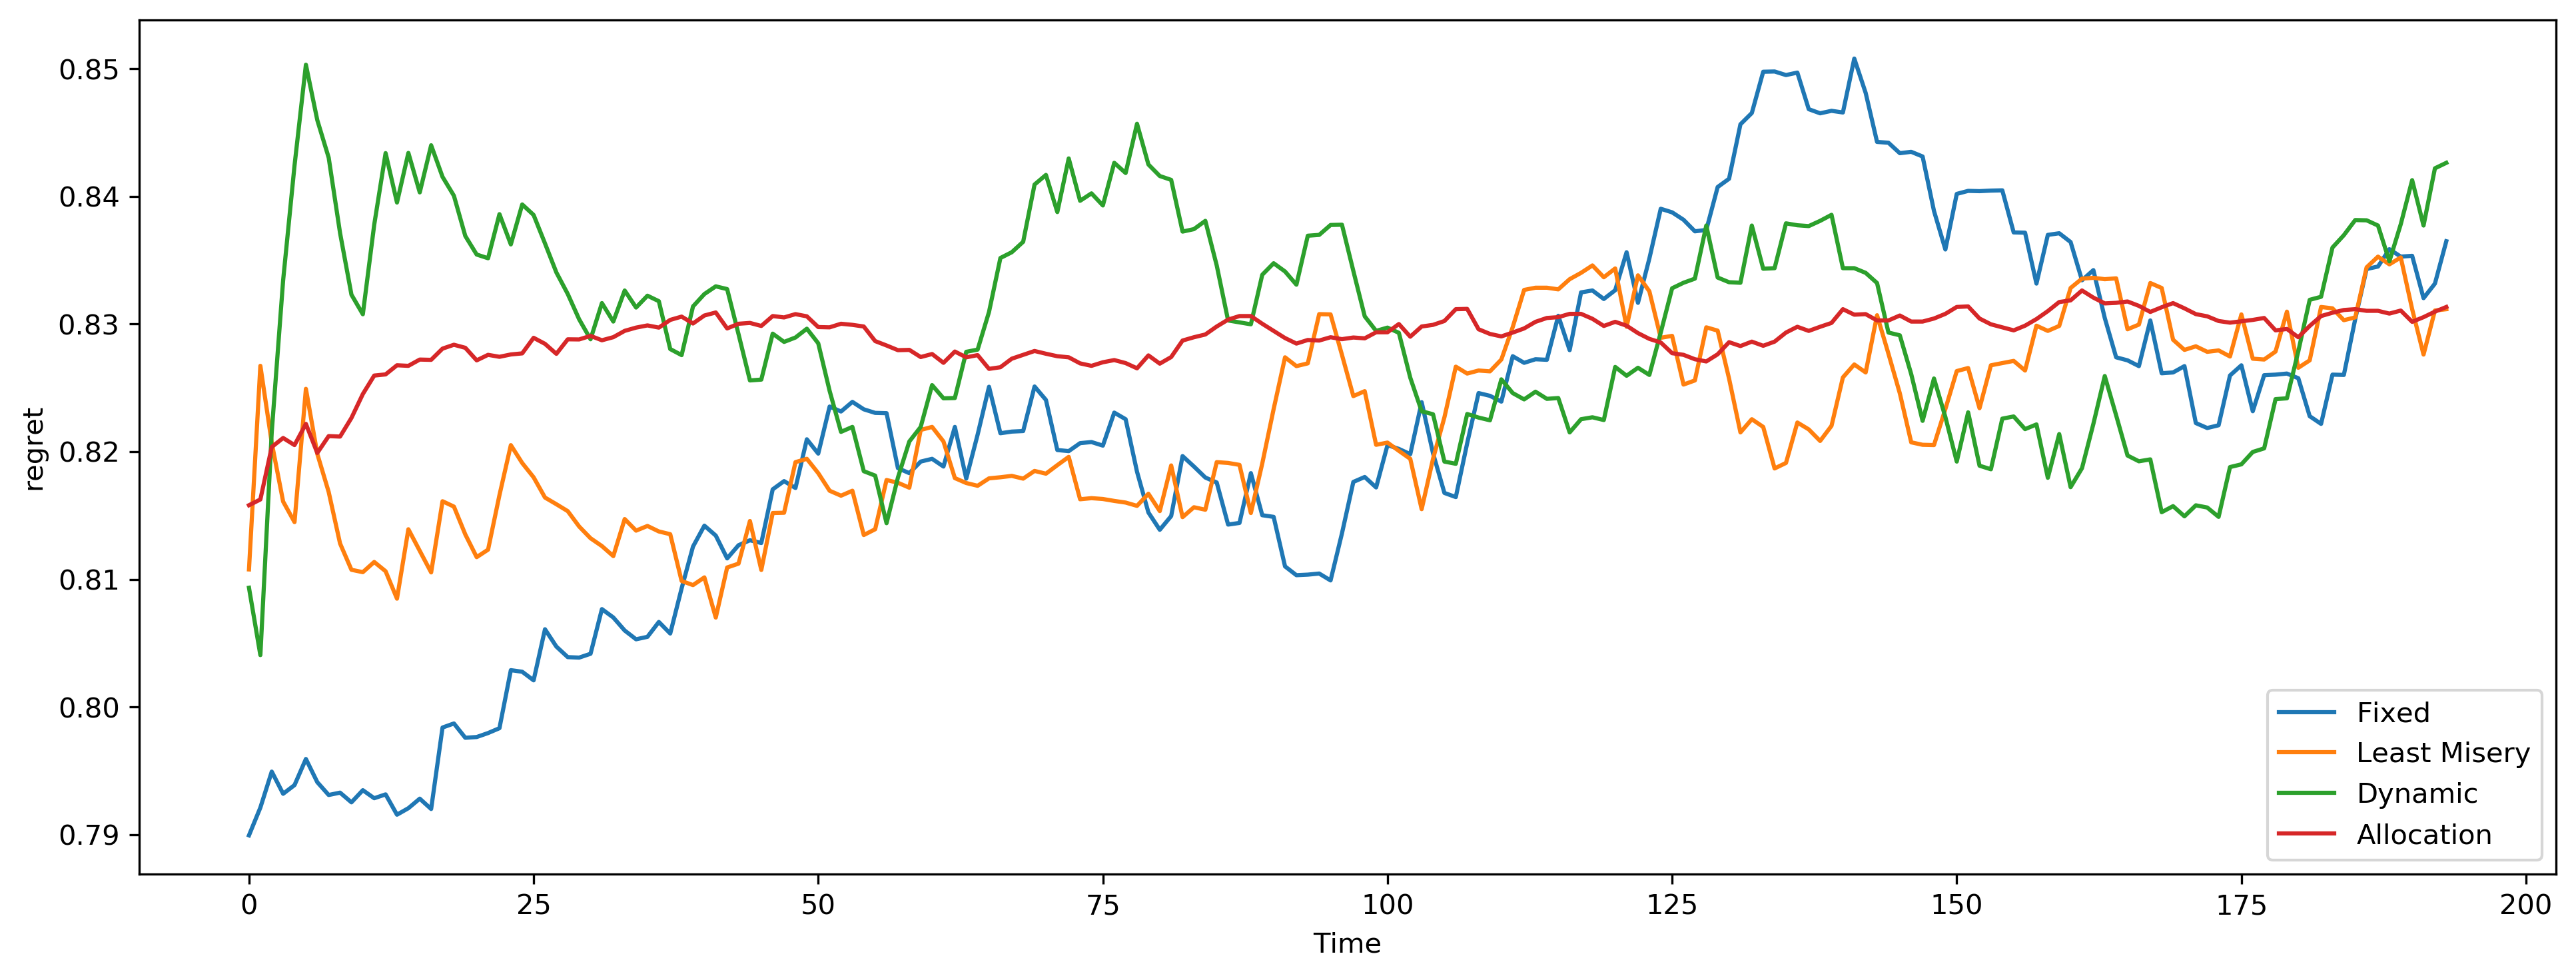
\includegraphics[width=4.5in]{imgs/dynfair/ml_avg_regret_overtime_sep20.png}
    \caption{MovieLens data set}
    \label{fig:local-regret-ML}
    \end{subfigure}
    \begin{subfigure}{1.0\textwidth}
    \centering
      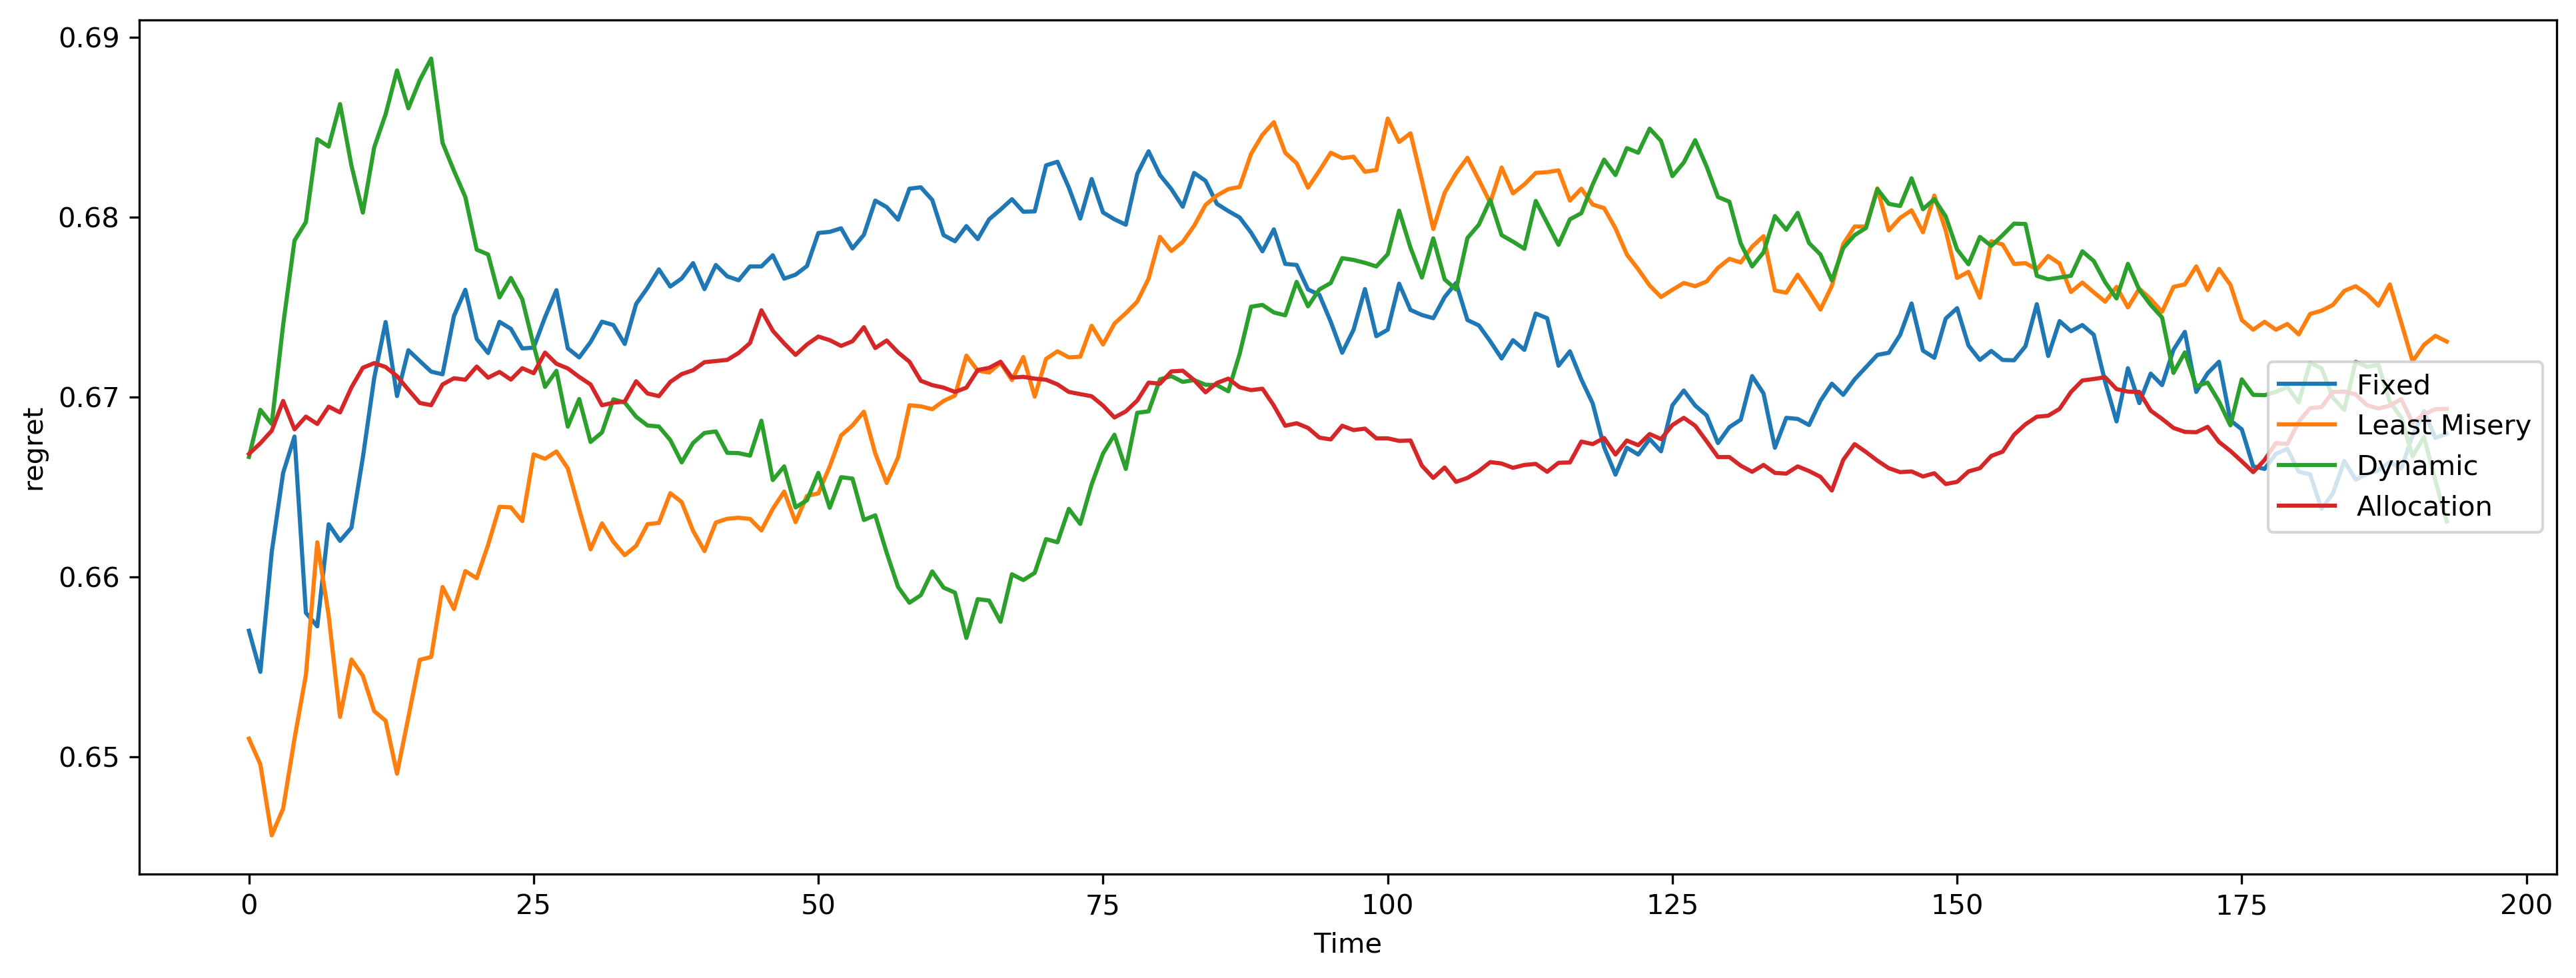
\includegraphics[width=4.5in]{imgs/dynfair/kiva_avg_regret_overtime_sep20.png}
    \caption{Kiva data set}
    \label{fig:local-regret-Kiva}
    \end{subfigure}
    \caption{Average fairness regret over time}
    \label{fig:local-regret}
\end{figure}

\begin{figure*}[t!]
    \centering
    \begin{subfigure}[t]{0.5\textwidth}
        \centering
        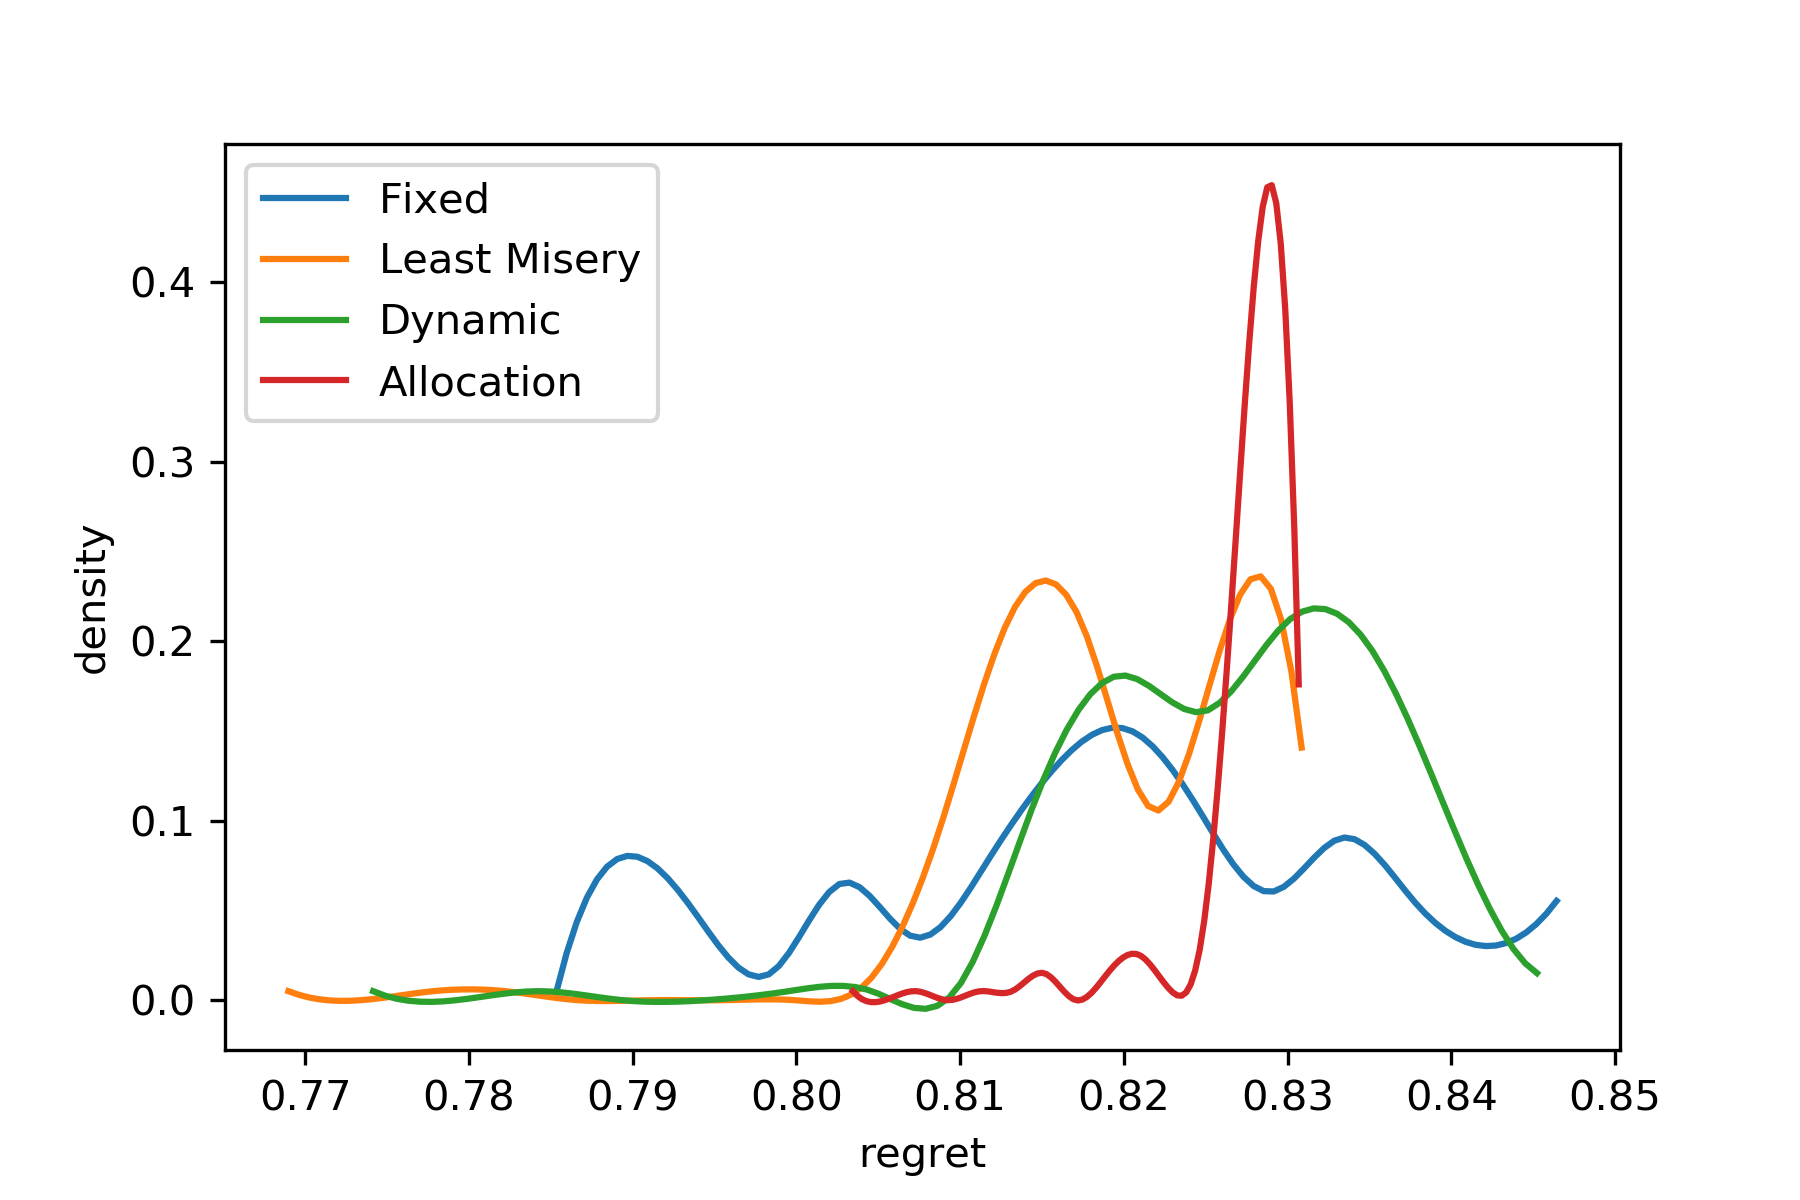
\includegraphics[width=3.0in]{imgs/dynfair/ML_regret_variance_sep20.png}
        \caption{MovieLens}
        \label{fig:local-regret-ML}
    \end{subfigure}%
    ~ 
    \begin{subfigure}[t]{0.5\textwidth}
        \centering
        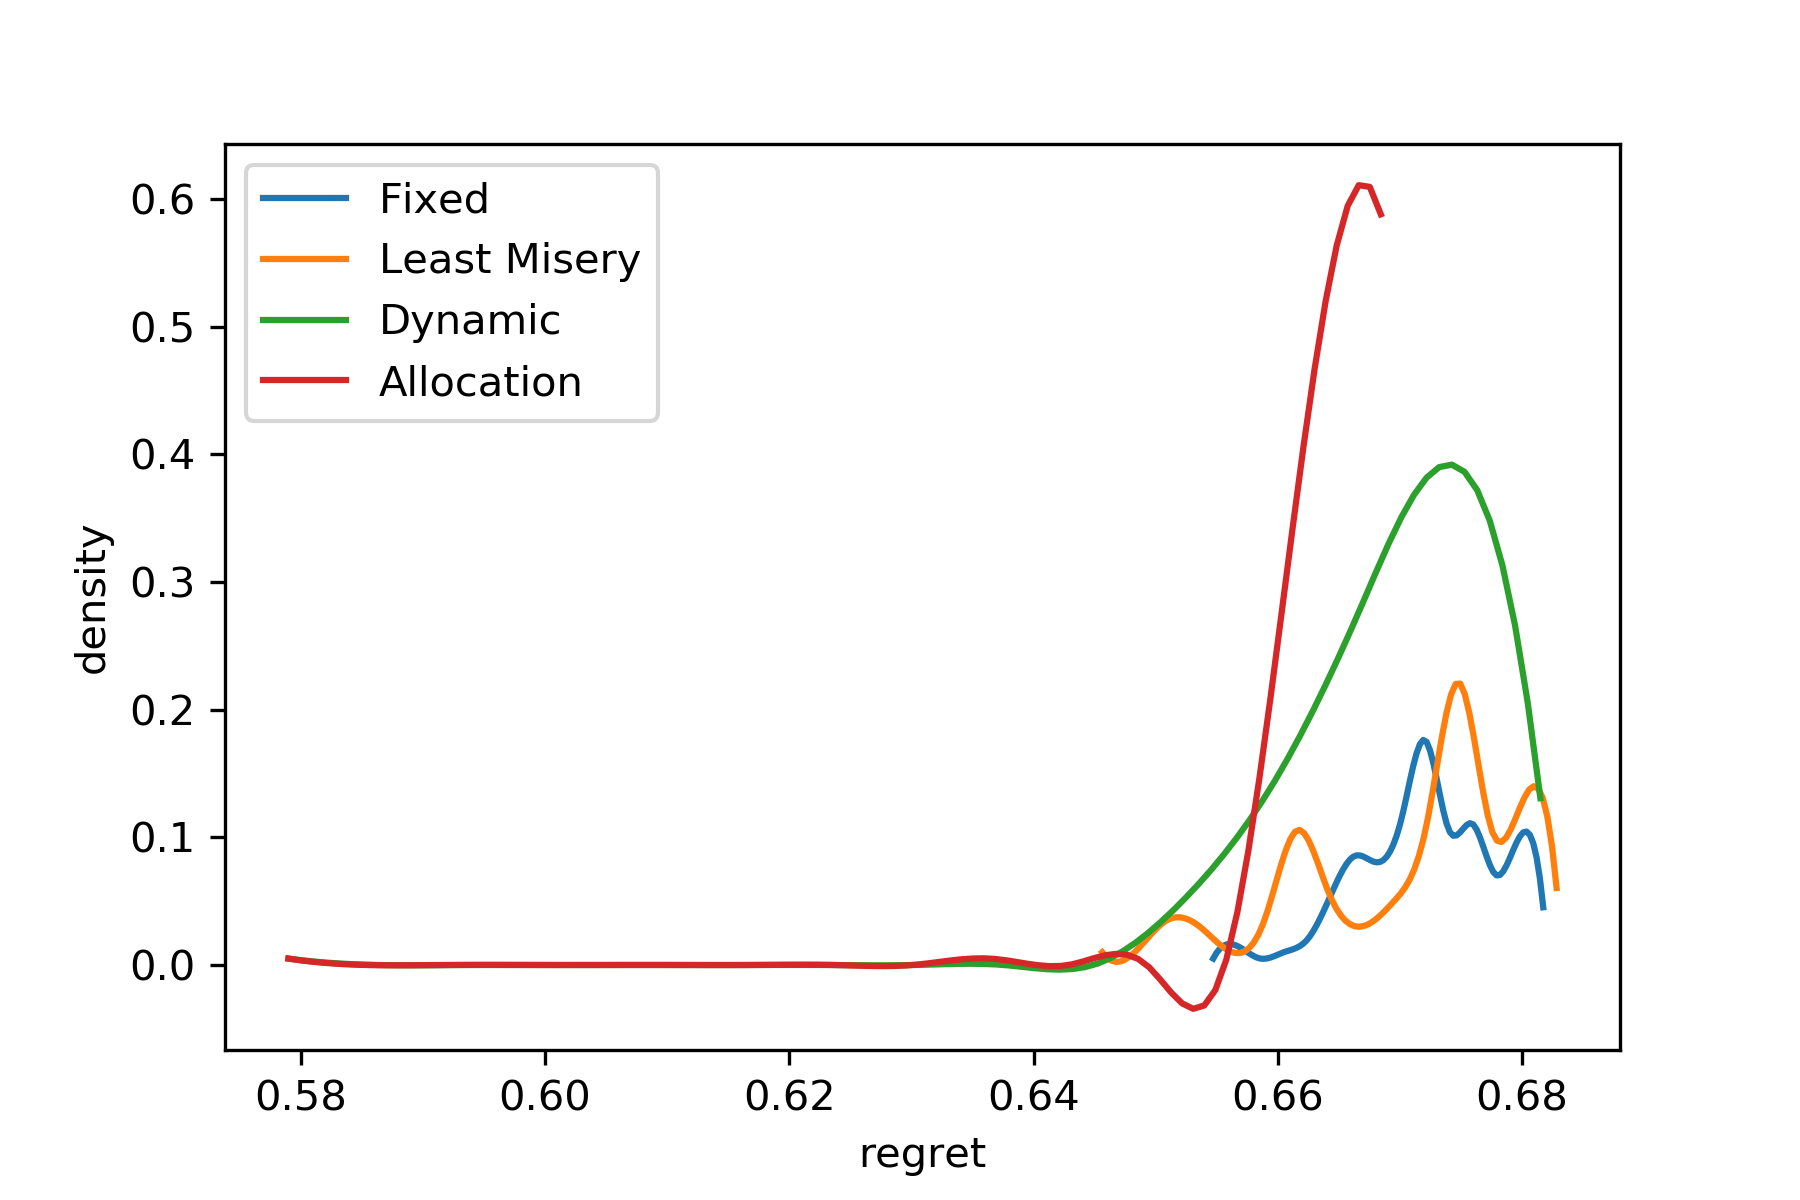
\includegraphics[width=3.0in]{imgs/dynfair/kiva_regret_variance_sep20.png}
        \caption{Kiva}
        \label{fig:local-regret-Kiva}
    \end{subfigure}
    \caption{Distribution of fairness regret}
\end{figure*}

Across both tables and in the time series figure, we see that the Allocation method has  lower variance in the fairness it achieves across iterations. Another way to see this consistency is the distribution of the average regret values. Figures~\ref{fig:local-regret-ML} and \ref{fig:local-regret-Kiva} show the distribution of regret for the different choice functions on each data set. The distribution of the Allocation method (shown in red) falls within a much narrower band than any of the other methods, particularly in the MovieLens data set where we see the Fixed method in blue taking on a wide range of regret values. At any given time, the Allocation algorithm is producing consistently fair results without the large variations in regret seen the other algorithms. As its fairness results are similar to those of the other lottery mechanisms, this consistency is a good reason to prefer it.

\subsection{Conclusion and Future Work}
In this paper, we conceptualize algorithmic fairness and recommendation fairness, in particular, as a problem of \textit{social choice}. That is, we define the task of computing a recommendation as a problem of arbitrating among the preferences of different individual agents to arrive at a single outcome. For our purposes, the agents in question include the user and also multiple \textit{fairness concerns} that may be active within a particular organization. 

The move to frame fairness as a problem of social choice has several important consequences. First, it highlights the multiplicity and diversity of fairness (and other stakeholder) concerns that might be relevant in a given application. This approach allows us to be agnostic to different definitions and metrics of fairness and does not impose any particular structure on stakeholder preferences.

Second, we are able to make use of the large body of research in computational social choice, including the study of fairness, that has emerged in the past decades. 

Building on these ideas, we demonstrate the SCRUF framework for dynamic adaptation of recommendation fairness using social choice to arbitrate between different re-ranking methods. We define a set of choice functions, ranging from a simple fixed lottery to an adaptation of the probabilistic serial mechanism, and demonstrate their performance on two data sets where multiple fairness concerns have been defined. We found relatively minor differences between the different lottery mechanisms, except that the Allocation mechanism, which takes user preferences over features into account, provides lower variance in fairness over time and therefore a more consistently fair output.



\section{Approach and Methodology}
% - librec-auto

Despite progress in recent years, reproducibility remains a challenge in recommender systems research \cite{beel2016towards}. Minor differences in parameters and experimental settings can yield incompatible results, which make it difficult to provide definitive answers about the relative properties of different algorithms. Progress in this area is supported by providing platforms on which comparative experiments can be conducted using declarative experimental configuration (so that experimental settings can be easily shared), with pre-implemented methodological workflows, and with a large library of algorithms for rapid benchmarking. 

In this section, I describe \libauto{}, an open-source command-line Python package providing a wrapper for the well-known LibRec 2.0 recommender systems algorithm library\footnote{www.librec.net}. My contributions to this project were the implementation and addition of in-processing and post-processing fairness algorithms and fairness metrics. The detail of each method is describe in the following section.

\subsection{Librec-auto}
% In \cite{mansoury2018automating}, we introduced \libauto{}, an open-source command-line Python package providing a wrapper for the LibRec 2.0 recommender systems algorithm library\footnote{www.librec.net}. 
This tool has been presented in \cite{mansoury2018automating} and provides an environment that supports automated experimentation. Therefore it supports reproducibility of research in recommendation algorithms.

Key advantages of \libauto{} were its ability to support typical research workflows, to offer a declaration configuration system, and to supplement experiment execution with the scripted production of human-friendly outputs including visualizations.

We have now extended this platform in a number of ways, particularly to support research in fairness-aware recommendation. \libauto{} now supports the current 3.0 version of the LibRec library and can take advantage of the new algorithms (including deep learning algorithms) found there. The \libauto{} project has also enhanced LibRec with a suite of metrics for measuring the fairness of recommendation outcomes. Most significantly, the tool now supports recommendation re-ranking, a common approach to enhancing fairness, diversity, and other non-accuracy properties of recommendation outcomes.

\subsubsection{\textbf{Core features}}
\hfill

LibRec 3.0 is a Java-based recommendation generation platform. It has been available to the recommender systems community since 2015 \cite{guo2015librec}, and has large library of implemented recommendation algorithms (more than 70 as of this writing). The platform supports a variety of evaluation metrics and evaluation methodologies. However, our experience indicates that for practical experimentation and reproducibility research, LibRec by itself is not sufficient. For example, intermediate computational outputs, such as recommendation results, cannot be reused as input for new evaluation metrics, requiring the re-execution of potentially lengthy experiment executions.

We developed \libauto{}\footnote{github.com/that-recsys-lab/librec-auto} to retain the benefits of working with LibRec while adding support for experimentation. A sketch of the functionality of \libauto{} is provided in Figure~\ref{fig:librec-auto}. As the figure indicates, LibRec is encapsulated and its various component elements are used to execute particular portions of the experimental workflow. In addition, the optional re-ranking component allows for the study of re-ranking algorithms not within the scope of LibRec's design. The key inputs are data and an XML-based configuration file. A particular study may consist of multiple experiments, all of which are configured at the same time in the configuration file. Configuration files are modular, so that, for example, multiple studies can share the same methodology elements, preventing inadvertent misconfiguration. 

Although the figure indicates a straight-line of execution, parallelism is built into \libauto{} at the level of experiment execution. Because experiments can have lengthy execution times, the post-processing phase allows for integration with messaging platforms, including Slack, so that experimenters are notified when their tasks are complete. These messages can include visualizations of experimental output, to provide a quick overview of results. 

\begin{figure}
    \centering
    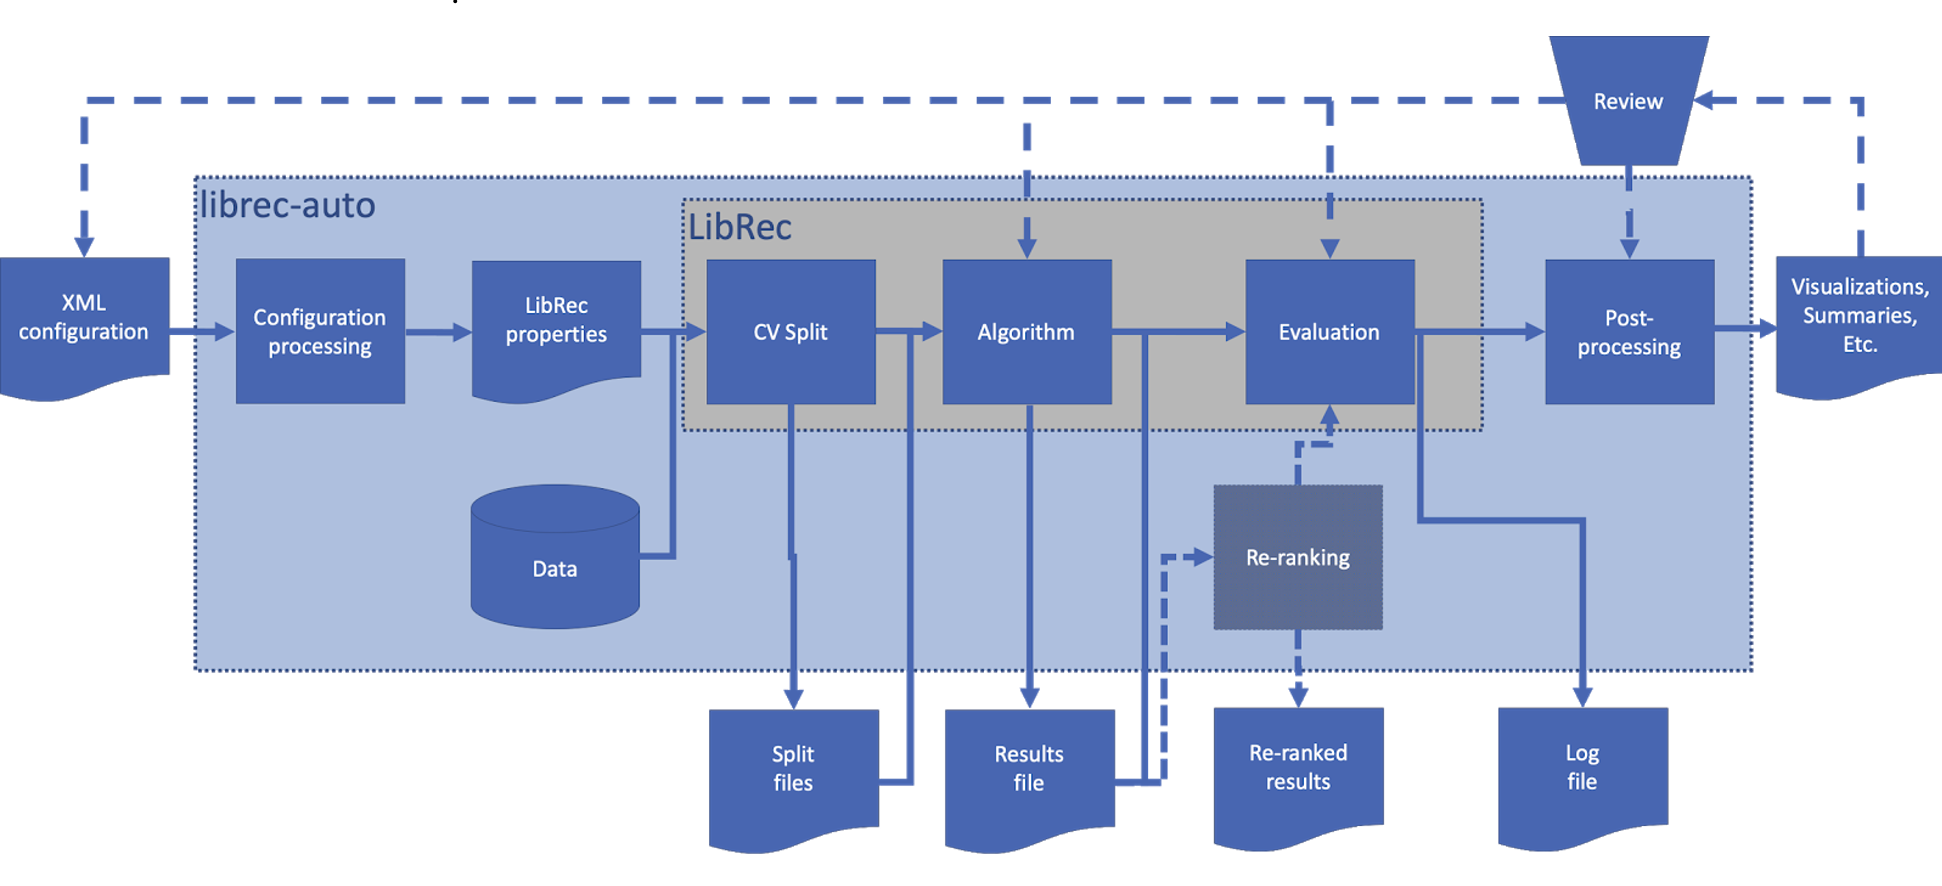
\includegraphics[width=5.25in]{imgs/la/librec-auto-diagram2.png}
    \caption{Schematic of experimentation workflow with \libauto{}. The LibRec library (Java, shown in grey) is encapsulated by \libauto{} (Python, shown in blue), which manages configuration, experimental outputs and post-processs. Added from \cite{mansoury2018automating} is the new re-ranking module shown in dark blue.}
    \label{fig:librec-auto}
    \vspace{-0.15in}
\end{figure}

\subsubsection{\textbf{Fairness-aware extensions}}
\hfill

Although \libauto{} has been under development since 2018, the latest release incorporates several key advances that specifically support common tasks in the study of recommendation fairness. These advances are (1) new evaluation metrics that report on fairness aspects of recommendation output, (2) an optional re-ranking step in the experiment pipeline, to support what is one of the most common category of fairness enhancing techniques, and (3) additional support for working with user (demographic) and item (content) features in algorithms and metrics. With these features, \libauto{} now can support a wide range of research activities in fairness-aware recommendation, and we will be adding additional capabilities in future releases.

Previously in the literature, many re-ranking algorithms have been proposed to achieve a balance between diversity and accuracy. The following methods try to achieve a fair representation between groups by penalizing the score of over-represented groups or reinforcing the score of the under-represented groups: (1) \textbf{FAR}, defined in \cite{liu2019farpfar}, combines a personalization-induced and fairness-induced scores with hyper-parameter $\lambda$; (2) \textbf{PFAR}, from \cite{liu2019farpfar}, adds a personalized weight to FAR, calculated based on item-features in user profile, representing the tolerance of the user for diverse resultsl and (3) \textbf{OFAiR} incorporates similar personalization and allows fine-grained control of protected group promotion when there are multiple protected groups \cite{sonboli2020opportunistic}. By contrast, (4) \textbf{FA*IR} \cite{zehlike2017fa} builds a queues of protected and unprotected items and draws from each queue to build the final re-ranked list. We also include two more general diversity-enhancing re-rankers first promoted in the information retrieval literature: (5) \textbf{MMR} diversifies result lists by greedily adding items with maximal marginal relevance \cite{carbonell1998use}, and (6) \textbf{XQuAD} defined in \cite{santos2010explicit} has similar goal to MMR algorithm, but it enhances diversity with respect to specific aspects. Finally, we include (7) \textbf{Calibrated Recommendations}, an algorithm closely tied to the Calibration metric above, which re-ranks recommendations to ensure a close match to the user's distribution of interests in item features~\cite{steck2018calibrated}. The re-ranking methods are part of \libauto{} and are implemented in Python.

Recommendation fairness and associated fairness metrics can be defined from the perspective of two main stakeholders: providers and consumers \cite{burke2017multisided}. Additionally, both provider-side and consumer-side metrics come in two basic varieties: exposure-based and hit-based. \textit{Exposure} metrics focus on the the appearance of protected items \cite{singh2018fairness} in a ranked list and \textit{hit-based} metrics take into account the suitability of the target user \cite{abdollahpouri2020multistakeholder}. Many metrics have been offered to measure recommendation fairness \cite{tsintzou2018bias,steck2018calibrated,beutel2019fairness,yao2017beyond,biega2018equity,castillo2019fairness,kuhlman2019fare,yang2017measuring}. We implement the following metrics in \libauto{} and where possible, both consumer-side and item-side versions of the metric are available: (1) \textbf{Discounted Proportional Fairness} (DPF), a hit-based fairness metric similar to the metric offered in \cite{castillo2019fairness} where it measures the ranking utility (nDCG) of the protected group with respect to the other groups. (2) \textbf{Calibration} \cite{steck2018calibrated}, a distribution-based metric that uses KL-Divergence to measure the difference in item category distribution between the preferences of users and their respective recommendation lists. (3) \textbf{Statistical parity}, based on the ideas discussed in \cite{zemel2013learning,ritov2017conditional}, measuring the difference in outcomes between protected and unprotected groups relative to various recommendation outcomes. Both ranking and prediction accuracy measures are supported. (4) \textbf{P-Percent-Rule} (PPR) discussed in \cite{biddle2006adverse}, is a two-sided extension of statistical parity \cite{barocas2016big}. (5) \textbf{Error-based} metrics proposed in Yao et al. \cite{yao2017beyond} including value-unfairness, absolute unfairness, underestimation unfairness, overestimation unfairness, and non-parity unfairness by Kamishima et al. \cite{kamishima2011fairness}. Additionally, we offer the following diversity-based metrics (6) \textbf{Intra-list distance (ILD)} \cite{ziegler2005improving}, a pairwise distance between all the item features in each user’s recommendation list, and (7) \textbf{Gini Index} calculated over the exposure of all the present groups in the recommendation list. All metrics are implemented in Java and integrated with the LibRec code base.

We plan future releases of \libauto{} to include integration with additional recommendation libraries, including LKPY~\cite{ekstrand2018lkpy}, LibFM~\cite{rendle2012factorization}, and DeepRec~\cite{zhang2019deeprec}.

\section{Proposed work and Timetable}
Overall, all of the presented methods in previous sections were looking to find a balance between accuracy and fairness either using a re-ranking methods or a regularization based method. Most of the focus of the previous methods were on reaching provider-side fairness. Here are the next steps for the previous projects.
\begin{itemize}
    \item \textbf{Fairness Survey}: Research on recommender systems fairness usually revolves around new algorithms. we are in the process of producing a journal article that surveys existing algorithms and compares their fairness properties on several data sets, from the perspective of both recommendation consumers and item providers. 

    We examine prominent examples from three different classes198of algorithms:  neighborhood-based, factorization using prediction loss, and factorization using ranking loss. From the neighborhood based algorithms we picked Sparse Linear Methods (SLIM) and item-based Knn. From the Matrix Factorization family using prediction loss we picked Biased Matrix Factorization, Weighted Regularized Matrix Factorization, Non-Negative Matrix Factorization, and from the factorization methods that use ranking loss we picked Bayesian Personalized Ranking. We are testing their fairness properties on the following datasets: The Movies Dataset, MovieLens 1M, Kiva dataset and Lastfm.
    
    we intend to submit this project to a journal.
    
    \item \textbf{Balanced Neighborhoods}: In this project, we built on the standard nearest neighbor techniques in recommender systems and built balanced neighborhoods to ensure diversity among the peers from whom recommendations are generated. In our future work for this project, we plan to extend these findings in several ways. We would like to have a more extensive experimentation of the fairness properties of the balanced neighborhood SLIM. And we would like to run these experimentation for both consumers and providers. We would also like to test this idea on different neighborhood-based methods besides SLIM. 
    
    It is possible that a multisided platform may require fairness be considered for both consumers and providers at the same time: a CP-fairness condition. For example, a rental property recommender may treat minority applicants as a protected class and wish to ensure that they are recommended properties similar to unprotected renters. At the same time, the recommender may wish to treat minority landlords as a protected class and ensure that highly-qualified tenants are referred to them at the same rate as to landlords who are not in the protected class. One important question for future research is how the outcomes for each stakeholder and the overall system performance are affected by combining consumer- and provider-fairness concerns.
    
    Finally, we expect to publish a journal article of these thorough experiments in the Information and Management Journal.
    
    \item \textbf{Dynamic Fairness}: In this paper, we conceptualized algorithmic fairness and recommendation fairness, in particular, as a problem of \textit{social choice}. That is, we define the task of computing a recommendation as a problem of arbitrating among the preferences of different individual agents to arrive at a single outcome. For our purposes, the agents in question include the user and also multiple \textit{fairness concerns} that may be active within a particular organization.
    
    The most important consequence of framing fairness as a problem of social choice is that it highlights the multiplicity and diversity of fairness (and other stakeholder) concerns that might be relevant in a given application. This approach allows us to be agnostic to different definitions and metrics of fairness and does not impose any particular structure on stakeholder preferences. The other important consequence is that we can use the extensive body of research on fairness in this field.
    
    We build the SCRUFF framework for dynamic adaptation of recommendation fairness using social choice to arbitrate between different re-ranking methods. We defined a set of choice functions, ranging from a simple fixed lottery to an adaptation of the probabilistic serial mechanism, and demonstrate their performance on two data sets where multiple fairness concerns have been defined. However, we found relatively minor differences between the different lottery mechanisms, except that the Allocation mechanism, which takes user preferences over features into account, provides lower variance in fairness over time and therefore a more consistently fair output.
    
    Therefore we intend to experiment with different aspects of this framework and test different aspects of it. Firstly, we intend to test different fairness definitions in this framework, test different base recommendation algorithms and re-ranking methods. The main reason behind that is that all these parts add extra restrictions to the framework and might hinder the results to change. Secondly, we didn't have an appropriate evaluation method to observe the results. We intend to use Generalized Cross Entropy for this purpose. Our results for fairness weren't bounded, therefore we intend to use Hinge Loss function to add a cap to the fairness values. Lastly, we intend to design a method that could guarantee certain fairness proportionality in the outputs.
    This Project is intended to be submitted to either the ACM Conference Series on Recommender Systems 2021 or the ACM conference on Fairness, Accountability, and Transparency 2021.
    
    
\end{itemize}



% \subsection{Fairness Survey}
% Research on recommender systems fairness usually revolves around new algorithms. we are in the process of producing a journal article that surveys existing algorithms and compares their fairness properties on several data sets, from the perspective of both recommendation consumers and item providers. 

% We examine prominent examples from three different classes198of algorithms:  neighborhood-based, factorization using prediction loss, and factorization using ranking loss. From the neighborhood based algorithms we picked Sparse Linear Methods (SLIM) and item-based Knn. From the Matrix Factorization family using prediction loss we picked Biased Matrix Factorization, Weighted Regularized Matrix Factorization, Non-Negative Matrix Factorization, and from the factorization methods that use ranking loss we picked Bayesian Personalized Ranking.
% We are testing their fairness properties on the following datasets: The Movies Dataset, MovieLens 1M, Kiva dataset and Lastfm.


% \subsection{Balanced Neighborhoods}
% % This paper extends ideas of fairness in classification to personalized recommendation. 
% Our BN-SLIM algorithm can be seen as an approach to building systems that target particular diversity-aware recommendation problems, where the providers and/or items can be divided into two disjoint categories. However, the approach is particularly suited to fairness-aware contexts because the objective function is optimized precisely when the protected and unprotected groups are weighted the same by the algorithm. 

% The most obvious precursor for this research is the work of Dwork et al. in the area of fair representation~\cite{zemel2013learning,fairness}. The authors propose learning a mapping between the individual instances in the data to prototype instances with balanced membership such that protected group identities are not recoverable. 

% This paper extends this idea of fairness in classification to personalized recommendation. However, our application of this concept is different in that we are building on the standard nearest neighbor techniques in recommender systems and building balanced neighborhoods to ensure diversity among the peers from whom recommendations are generated. 

% A key aspect of this extension is to note the tension between a personalized view of recommendation delivery and a regulatory view that values particular outcomes. The regulatory view is somewhat foreign to research in personalization, but there are strong arguments that total obedience to user preference is not always risk-free or desirable~\cite{pariser2011filter,sunstein2009republic}. This paper also introduces the concept of multisided fairness, relevant in multisided platforms that serve a matchmaking function. We identify consumer- and provider- fairness as properties desirable in certain applications and demonstrate that the concept of balanced neighborhoods in conjunction with the well-known sparse linear method can be used to balance personalization with fairness considerations.

% In our future work, we plan to extend these findings in several ways. It is possible that a multisided platform may require fairness be considered for both consumers and providers at the same time: a CP-fairness condition. For example, a rental property recommender may treat minority applicants as a protected class and wish to ensure that they are recommended properties similar to unprotected renters. At the same time, the recommender may wish to treat minority landlords as a protected class and ensure that highly-qualified tenants are referred to them at the same rate as to landlords who are not in the protected class. One important question for future research is how the outcomes for each stakeholder and the overall system performance are affected by combining consumer- and provider-fairness concerns.

% Another path to pursue is to have a more extensive experimentation of the fairness properties of the balanced neighborhood SLIM for both consumers and providers. We would like to test this idea on K-nearest neighbor method as well. Finally, we expect to publish a journal article of these thorough experiments in the Information and Management Journal.

% Another important area of research is to extend our measures of fairness. The additive measures used in this paper capture an aggregate representation of how recommendation results are changing for user and provider groups generally, but they do not permit fine-grained analysis of the tradeoffs experienced by individual users or providers. We do not know, for example, if the results of our Kiva.org experiments represent a Pareto improvement in system performance or just an average improvement over the stakeholder groups, and whether some subgroups are impacted more than others.

% One of the key challenges in this area is the domain-specificity of recommendation environments. The utilities that are delivered to each class of stakeholder are highly dependent on the type of item being recommended, the social function of the platform, and the interactions that it enables. It is therefore difficult to find appropriate data sets for experimentation and challenging to generalize across recommendation scenarios. 


% expanding balanced neighborhood on the provider-side fairness

% \subsection{Fairness-Aware Re-ranking / Personalized Fairness-Aware Re-ranking}

% In this work, we proposed a personalized fairness-aware re-ranking algorithm for microlending that can balance accuracy and fairness. We increase the coverage rate of borrowers' regions for Kiva.org to achieve borrower-side fairness, and we show that our algorithm can do so with minimal loss in ranking accuracy. In addition, our algorithm includes lender-specific weights that can be used to personalize the degree of loan diversity.

% In the future, we will consider the position bias into the fairness-aware recommendation for microlending. As discussed in this paper, the recommendation for microlending is moved forward by considering the coverage rate of borrowers and the lenders' diversity tolerance. However, the top positions are generally more valuable than the bottom ones \cite{robertson1977probability}. We plan to make a further assumption that the chance of exposure for an item depends on its position in ranking. Thus, incorporating such position bias into the re-ranking criteria for microlending is promising.

% In the future, we will study a number of variants of our algorithms presented here. We plan to explore different methods for computing personalized diversity tolerance factors, especially to solve the cold-start problem in the current algorithm. We also plan to examine variants of the re-ranking algorithm to take into account the size of each provider group's inventory. 

% FAR/PFAR is extremely strict in its requirement that each possible provider group appears at least once at the top of the list. Therefore, another variant to consider is one that can adjust the accuracy/fairness tradeoff in a dynamic way as items are ranked, valuing accuracy more at the top of the list and provider-side fairness more at the bottom of the list.

% Finally, we note that, in real-world recommendation applications, managing the tradeoff between accuracy and coverage of provider groups is not a single-shot process. Rather it is an online process, where a current lack of coverage can be compensated for at a later time, and where results are evaluated temporally. This would require making the algorithm sensitive to historical patterns of coverage, rather than just the results obtained in the current list. We intend to explore this type of algorithm design and evaluation in our future work.

% This project currently is an on-going project and we intend to develop a method using probabilistic serial allocation and submit it to the ACM Conference Series on Recommender Systems 2021.

% \subsection{Opportunistic Multi-aspect Fairness through Personalized Re-ranking}
% The results of our experiments show that OFAiR works as intended. Its proportion-based MMR model provides a much better tradeoff between ranking accuracy and fairness for the protected-unprotected case than the FAR/PFAR models explored in prior work. In the datasets under study, we show that users' tolerance for diversity varies across features, which justifies our approach of differentiating users based on the opportunities they represent for enhancing provider-side fairness. 

% We show that the combination of personalized, feature-specific, weights together with weights identifying protected feature values is effective with the feature-specific tolerance helping maintain accuracy and the feature weight promoting protected group items. As we showed, our method can be applied across multiple protected groups at the same time and can ensure fairness with respect to system's designed fairness goal for each feature.

% One of the challenges in this work is the lack of proper datasets that have user features and these datasets are specifically lacking in domains where fairness matters. Due to this issue, we chose the Movies dataset to show the capabilities of our method.

% As our future work in this section, we intend to run a more thorough experimentation with weights of the weighted cosine similarity and capture the influence of these weights on the final results. We also intend to use different recommendation algorithms as the base recommendation.

% A more general method to use is the metric learning approach, that assumes different dimensions and assigns weights to these dimensions accordingly. This is useful as it automatically assigns weights to dimensions not manually.

% The other approach to explore is to use voting methods in the fair resource allocation literature in the computational social choice field. Specifically, the cake cutting problem, where we want to allocate cake slices fairly where we assume users have different preferences for different layers of the cake which is similar to our research problem here, where users have different preferences over different dimensions.

% The results of this experimentation is intended to be submitted to the ACM FAcct 2021 conference.

% journal

% In our next work, we intend to explore further the idea of ``opportunity'' in subgroup-fairness-aware recommendation. In particular, when recommendations are delivered over time, prior outcomes relative to different protected groups may dictate what opportunities should be most salient at any given moment. We intend to publish this work later this year in The ACM Series on Recommender Systems.


% \subsection{Dynamic Fairness}
% In this paper, we conceptualize algorithmic fairness and recommendation fairness, in particular, as a problem of \textit{social choice}. That is, we define the task of computing a recommendation as a problem of arbitrating among the preferences of different individual agents to arrive at a single outcome. For our purposes, the agents in question include the user and also multiple \textit{fairness concerns} that may be active within a particular organization. 

% The move to frame fairness as a problem of social choice has several important consequences. First, it highlights the multiplicity and diversity of fairness (and other stakeholder) concerns that might be relevant in a given application. This approach allows us to be agnostic to different definitions and metrics of fairness and does not impose any particular structure on stakeholder preferences.

% Second, we are able to make use of the large body of research in computational social choice, including the study of fairness, that has emerged in the past decades. 

% Building on these ideas, we demonstrate the SCRUFF framework for dynamic adaptation of recommendation fairness using social choice to arbitrate between different re-ranking methods. We define a set of choice functions, ranging from a simple fixed lottery to an adaptation of the probabilistic serial mechanism, and demonstrate their performance on two data sets where multiple fairness concerns have been defined. We found relatively minor differences between the different lottery mechanisms, except that the Allocation mechanism, which takes user preferences over features into account, provides lower variance in fairness over time and therefore a more consistently fair output.

% %%%%%%%%%%%%%%%%%%%%%%%%%%%%%

% What evaluation function fits the dynamic fairness environment
% What's regret in this environment
% Using hinge loss for the objective function to bound the fairness achievement etc.
% trying out different fairness definitions
% designing a method that guarantees certain properties in the re-ranked list



\bibliographystyle{ACM-Reference-Format}
\bibliography{myref.bib}
\end{document}
